%%
% The BIThesis Template for Bachelor Graduation Thesis
%
% 北京理工大学毕业设计(论文) —— 使用 XeLaTeX 编译
%
% Copyright 2021-2023 BITNP
%
% This work may be distributed and/or modified under the
% conditions of the LaTeX Project Public License, either version 1.3
% of this license or (at your option) any later version.
% The latest version of this license is in
%   http://www.latex-project.org/lppl.txt
% and version 1.3 or later is part of all distributions of LaTeX
% version 2005/12/01 or later.
%
% This work has the LPPL maintenance status `maintained'.
%
% The Current Maintainer of this work is Feng Kaiyu.
%
% Compile with: xelatex -> biber -> xelatex -> xelatex

% 开启盲审格式 blindPeerReview=true (如:[type=bachelor,blindPeerReview=true])

\documentclass[type=bachelor]{bithesis}

\BITSetup{
  cover = {
    % 在封面中载入有「北京理工大学」字样的图片,如无必要请勿改动。
    headerImage = images/header.png,
    % 在封面标题中使用思源黑体,使用此选项可以保证与 Word 封面标题的字体一致。
    xiheiFont = STXIHEI.TTF,
    %% 使用以下参数来自定义封面日期
    % date = 2022年6月,
  },
  info = {
    % 想要删除某项封面信息,直接删除该项即可。
    % 想要让某项封面信息留空(但是保留下划线),请设置为空字符串。
    % 如需要换行,则用 “\\” 符号分割。
    title = 基于深度学习和聚类优化多实例点云配准,
    titleEn = {Optimized Multi-Instance Point Cloud Registration 
    based on Deep Learning and Cluster Methods},
    school = \quad 自动化学院 \quad,
    major = 自动化,
    author = 杨润一,
    class = 06111902,
    studentId = 1120191211,
    supervisor = 由育阳,
    keywords = {点云配准; 多实例; 聚类; 点对匹配; 深度学习; 对比学习},
    keywordsEn = {Point Cloud Registration; Multi-instance; Clustering; Point Cloud Correspondence; Deep Learning; Contrastive Learning},
    % 如果你的毕设为校外毕设,请将下面这一行语句解除注释(删除第一个百分号字符)并填写你的校外毕设导师名字
    % externalSupervisor = 左偏树,
  },
  style = {
    % 保持参考文献的缩进样式与 Word 模板一致。
    % 如果你不需要此样式,请将此行注释掉。
    bibliographyIndent = false,
  }
}

% 使用 listings 宏包进行代码块使用,并使用了预定义的样式,
% 你也可以选用自己的喜欢的其他宏包,如 minted;
% 然而由于 minted 依赖 Python 的 Pygments 库作为外部依赖,因此出于模板的简洁程度考虑,我们没有提供 minted 进行代码块书写的示例。
\usepackage{listings}
\usepackage{booktabs}
\usepackage{bbm}
\usepackage{float}
\usepackage{caption}
\usepackage{subcaption}
\usepackage{graphicx}
\usepackage{amsmath}
\usepackage{amssymb}
\usepackage{amsfonts}
\usepackage{booktabs}
\usepackage{gensymb}
\usepackage[
  backend=biber,
  style=gb7714-2015,
  gbalign=gb7714-2015,
  gbnamefmt=lowercase,
  gbpub=false,
  doi=false,
  url=false,
  eprint=false,
  isbn=false,
]{biblatex}

% 参考文献引用文件位于 misc/ref.bib
\addbibresource{misc/ref.bib}


% 文档开始
\begin{document}

% 标题页面:如无特殊需要,本部分无需改动
\MakeCover

% 原创性声明:如无特殊需要,本部分无需改动
% 更改为 PDF 页面插入,如需要添加内容,可考虑先用 Word 制作再覆盖 misc/1_originality.pdf
% ====== 原创性声明(PDF 格式)======
\begin{blindPeerReview}
  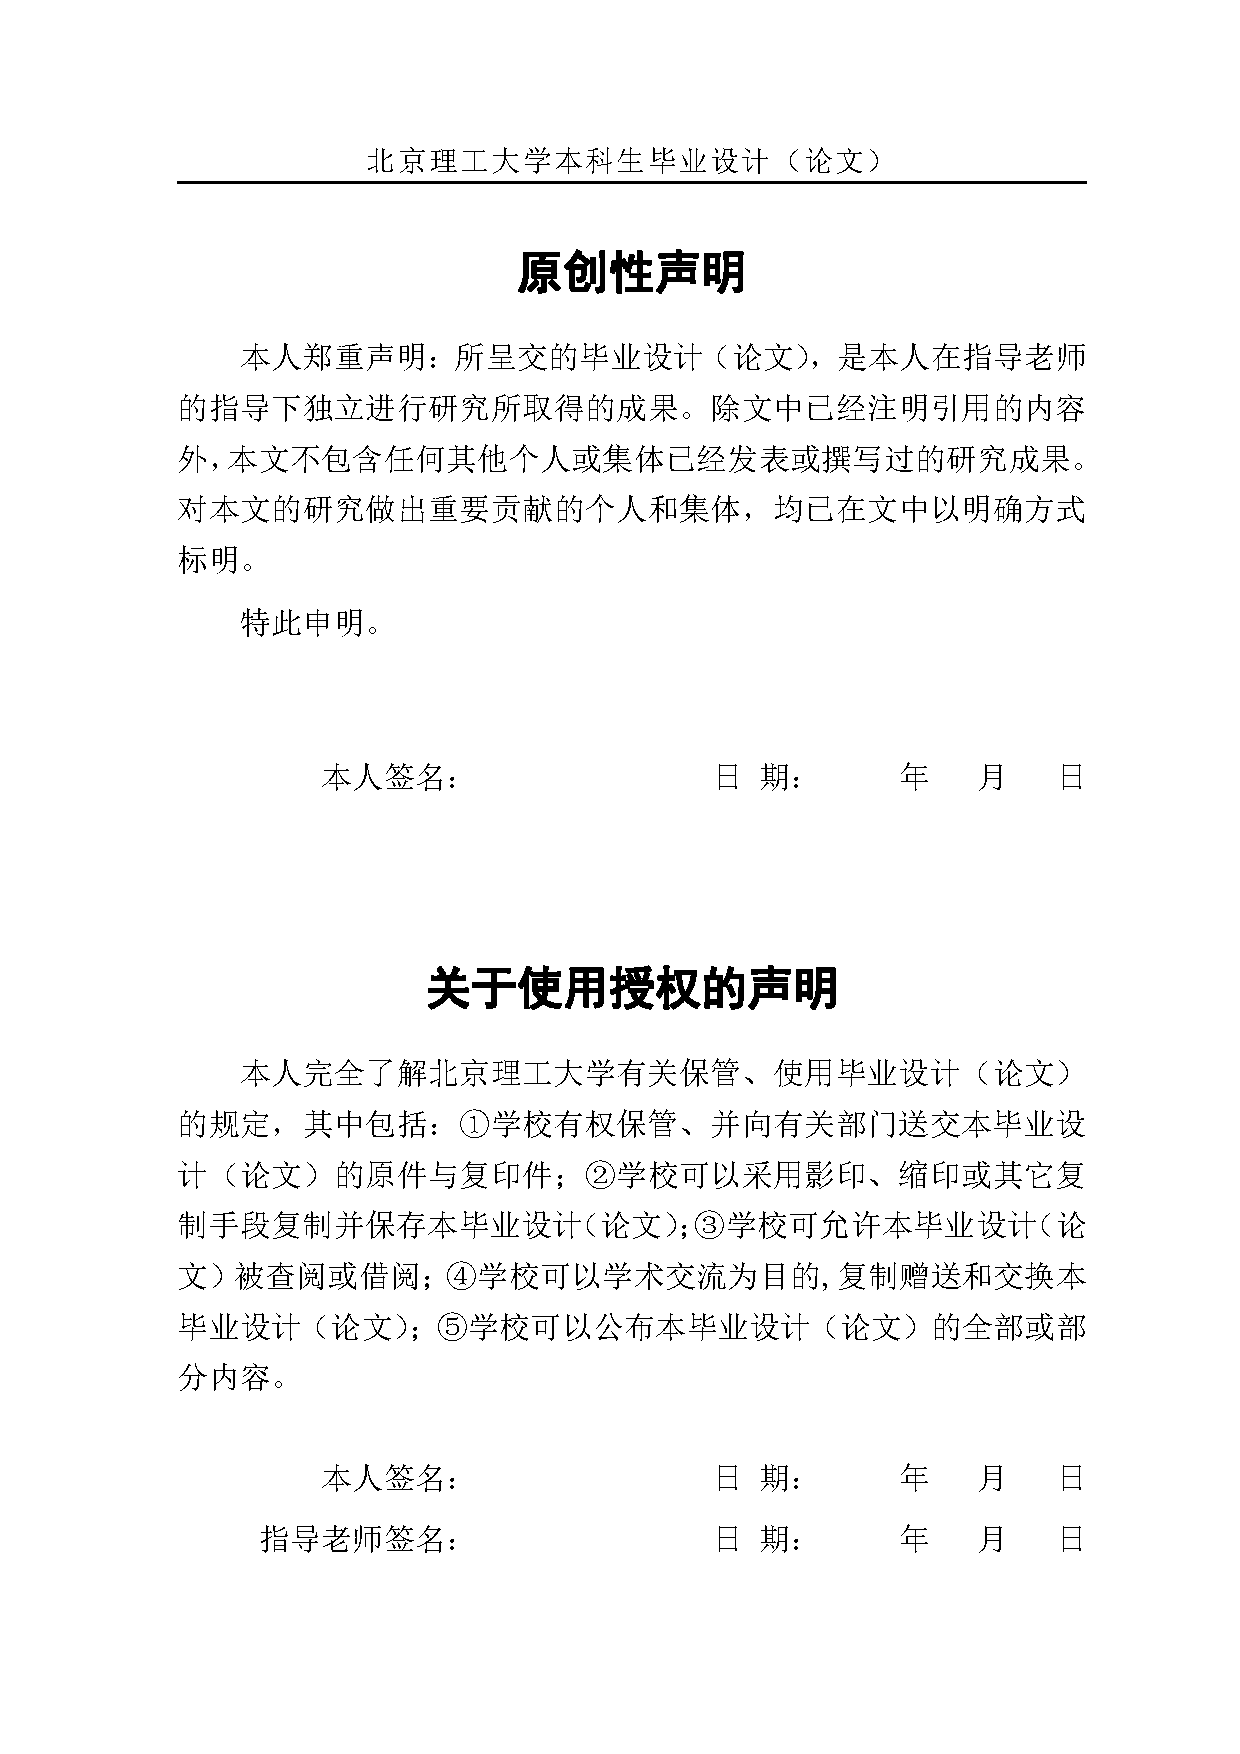
\includepdf{misc/1_originality.pdf}\newpage
\end{blindPeerReview}
% ====== 原创性声明(PDF 格式)======
% ====== 原创性声明(LaTeX 格式)======
% %%
% The BIThesis Template for Bachelor Graduation Thesis
%
% 北京理工大学毕业设计(论文)原创性声明模板 —— 使用 XeLaTeX 编译
%
% Copyright 2020-2023 BITNP
%
% This work may be distributed and/or modified under the
% conditions of the LaTeX Project Public License, either version 1.3
% of this license or (at your option) any later version.
% The latest version of this license is in
%   http://www.latex-project.org/lppl.txt
% and version 1.3 or later is part of all distributions of LaTeX
% version 2005/12/01 or later.
%
% This work has the LPPL maintenance status `maintained'.
%
% The Current Maintainer of this work is Feng Kaiyu.
%
% Compile with: xelatex -> biber -> xelatex -> xelatex
%
% 如无特殊需要,本页面无需更改

\MakeOriginality

% ====== 原创性声明(LaTeX 格式)======

% 前置页面定义
\frontmatter
% 摘要:在摘要相应的 TeX 文件处进行摘要部分的撰写
%%
% The BIThesis Template for Bachelor Graduation Thesis
%
% 北京理工大学毕业设计(论文)中英文摘要 —— 使用 XeLaTeX 编译
%
% Copyright 2020-2023 BITNP
%
% This work may be distributed and/or modified under the
% conditions of the LaTeX Project Public License, either version 1.3
% of this license or (at your option) any later version.
% The latest version of this license is in
%   http://www.latex-project.org/lppl.txt
% and version 1.3 or later is part of all distributions of LaTeX
% version 2005/12/01 or later.
%
% This work has the LPPL maintenance status `maintained'.
%  
% The Current Maintainer of this work is Feng Kaiyu.

% 中英文摘要章节
\begin{abstract}
    三维点云配准是点云处理中的一项基本任务,其在机械臂、自动驾驶、自主运动机器人、即时定位与地图构建(Simultaneous Localization and Mapping,SLAM)等众多基于视觉方法的应用中起着关键的作用。随着人工智能、元宇宙、自动驾驶等技术的兴起,将深度学习应用于点云配准的工作已经日趋成熟。目前大多数点云配准任务研究主要集中在成对配准上。然而,在实际应用中,目标场景可能包含多个重复实例,我们需要估计模板点云与目标点云中这些重复实例之间的多个刚性变换,也就是多实例点云配准。

    本文针对三维点云配准问题,特别是多实例点云配准,进行了深入研究。我们调研并整理了多实例点云配准的国内外研究现状,并总结了前人研究的优势和劣势。现有解决方案需要对大量假设进行采样以检测可能的实例并排除异常值,当实例和异常值的数量增加时,其鲁棒性和效率会显着降低。我们建议根据距离不变矩阵将噪声对应集直接分组到不同的簇中。通过聚类自动识别实例和异常值,达到稳健且快速表现。
    
    基于这一研究背景,我们提出了新的多实例点云配准架构,高效对应聚类的多实例点云配准 (ECC) 。分析聚类方法的点云配准,发现对于描述子的依赖性高,离群点比例高的时候效果会大大下降,所以我们提出了基于深度学习和聚类优化的多实例点云配准 (DMR),首先利用对比学习来学习输入推定对应关系的分布良好的深度表示。然后基于这些表示,我们提出了异常值修剪策略和聚类策略,以有效地删除异常值并将剩余的对应关系分配给正确的实例,达到了更好的效果。
    
    综上所述,我们的研究表明,基于深度学习的多实例点云配准方法在处理复杂的多实例点云配准问题上具有优秀的性能,提供了新的研究思路和方法。
    
\end{abstract}

% 英文摘要章节
\begin{abstractEn}
    Three-dimensional point cloud registration is a fundamental task in point cloud processing, which plays a crucial role in a wide range of vision-based applications such as robotic arms, autonomous driving, autonomous mobile robots, and Simultaneous Localization and Mapping (SLAM). With the rise of artificial intelligence, metaverse, autonomous driving, and other technologies, the application of deep learning to point cloud registration has become increasingly mature. Current research on point cloud registration mostly focuses on pairwise registration. However, in practical applications, the target scene may contain multiple repeated instances, and we need to estimate multiple rigid transformations between the template point cloud and these repeated instances in the target point cloud, that is, multi-instance point cloud registration.

    This paper conducts in-depth research on the problem of three-dimensional point cloud registration, especially multi-instance point cloud registration. We have surveyed and summarized the domestic and international research status of multi-instance point cloud registration and summarized the advantages and disadvantages of previous studies. Existing solutions require sampling a large number of hypotheses to detect possible instances and reject outliers, and their robustness and efficiency degrade significantly when the number of instances and outliers increases. We propose to directly group the noisy correspondence set into different clusters based on a distance invariance matrix. Through clustering, instances and outliers are automatically identified, achieving robust and fast performance.
    
    Based on this research background, we propose a new multi-instance point cloud registration framework, \textbf{E}fficient \textbf{C}orrespondence \textbf{C}lustering for Multi-instance Point Cloud Registration (\textbf{ECC}). After analyzing the point cloud registration of the clustering method, we find that the effect will drop significantly when it has high dependency on the descriptor and a high proportion of outliers. Therefore, we propose \textbf{D}eep Learning and Cluster Opimisation based \textbf{M}ulti-instance Point Cloud \textbf{R}egistration (\textbf{DMR}), which first uses contrastive learning to learn a good deep representation of the input estimation correspondence. Then, based on these representations, we propose an outlier pruning strategy and a clustering strategy to effectively remove outliers and allocate the remaining correspondences to the correct instances, achieving better results.
    
    In conclusion, our research shows that the deep learning-based multi-instance point cloud registration method has excellent performance in dealing with complex multi-instance point cloud registration problems and provides new research ideas and methods.
\end{abstractEn}


\MakeTOC

% 正文开始
\mainmatter

% 第一章
%%
% The BIThesis Template for Bachelor Graduation Thesis
%
% 北京理工大学毕业设计(论文)第一章节 —— 使用 XeLaTeX 编译
%
% Copyright 2020-2023 BITNP
%
% This work may be distributed and/or modified under the
% conditions of the LaTeX Project Public License, either version 1.3
% of this license or (at your option) any later version.
% The latest version of this license is in
%   http://www.latex-project.org/lppl.txt
% and version 1.3 or later is part of all distributions of LaTeX
% version 2005/12/01 or later.
%
% This work has the LPPL maintenance status `maintained'.
%
% The Current Maintainer of this work is Feng Kaiyu.
%
% 第一章节

\chapter{绪论}

\section{研究背景和意义}
% 这里插入一个参考文献,仅作参考

\subsection{三维点云配准}
21世纪以来,人工智能技术的发展对于社会有着重大的影响,智能化成为工程技术突破的内核。机器能够进行快速计算、存储和处理大量数据,并通过互联网将社会连为一体。现在由人工智能驱动的新一代机器,它们可以越来越自主地解决复杂的任务,其中以视觉为核心的机器技术快速发展,机械臂、自动驾驶、自主运动机器人等进入了人们的视野。随着2012年AlexNet\cite{krizhevsky2017imagenet} 问世以来,深度学习方法打开了计算机视觉的新大门。越来越多的深度学习方法比如VGG\cite{simonyan2014very} 、ResNet\cite{he2016deep} 、ViT\cite{dosovitskiy2020image} 被用在了图像分类、分割、场景理解等任务中。为了更好的理解真实世界,人们开始尝试将深度学习方法用于三维数据中,随着激光雷达和Kinect等高精度传感器的快速发展,点云已经成为表示三维世界的主要数据格式。2017年PointNet\cite{qi2017pointnet} 出现后,深度学习方法也同样被广泛应用在了点云处理中。

三维点云配准是点云处理中的一项基本任务\cite{qi2017pointnet,huang2021comprehensive,besl1992method} ,其在机械臂、自动驾驶、自主运动机器人等众多基于视觉方法的应用中起着关键的作用。首先是三维重建,生成完整的三维场景是各种计算机视觉应用的基础和重要技术,包括自动驾驶中的高精度三维地图重建、机器人技术中的三维环境重建等。例如,配准可以为机器人应用程序中的路线规划和决策构建三维环境。

其次,三维场景中的定位。三维场景中的定位和重定位对于机器人技术尤其重要。例如,无人驾驶汽车会估计其在地图上的位置及其与道路边界线的距离。点云配准可以将当前的实时三维视图与其所属的三维环境准确匹配,提供高精度定位服务。此应用表明,点云配准提供了机器和三维环境交互一种解决方案。

第三,位姿估计。将点云A与另一个点云B对齐可以生成与点云B相关的点云A的位姿信息。这个位姿信息可用于机器人决策。例如,点云配准可以获取环境中物体的位姿信息,以决定机械臂移动到哪里以准确抓取并移动物体。位姿估计为机器人三维环境理解提供了重要信息。

在国防安全、信息安全、环境安全等领域,无人机系统、自主导航、环境感知等技术应用愈发广泛。在这些应用中,点云配准也发挥着重要作用。例如,无人机系统需要对目标进行跟踪,而点云配准可以提供目标的位姿信息,来实现目标跟踪。点云配准可以用于环境感知,用于分割、检测、识别等任务,从而实现环境感知。在自动驾驶、机器人自主导航中,高精度的点云配准算法可以提供高精度的3D地图场景重建,为自主机器提供视觉定位、路径规划、障碍物检测等技术保障\cite{zidongjiashilujingguihua} 。


\subsection{多实例点云配准}
点云配准旨在通过对源点云和目标点云之间进行刚性变换,使得源点云和目标点云尽可能重合。点云配准的输入是两个点云,输出是一个刚性变换矩阵。点云配准的目标是找到一个刚性变换矩阵,使得源点云和目标点云之间的距离最小。传统方法中,一般流程为查找匹配点,通过SVD等方法求解出变换矩阵。随着机器学习和深度学习算法的广泛使用,基于深度学习方法和组合优化方法进一步提高了点云配准的准确率\cite{deng2018ppf,deng2018ppfnet,qin2022geometric} 。

\begin{figure*}[ht]
    \vspace{-4mm}
    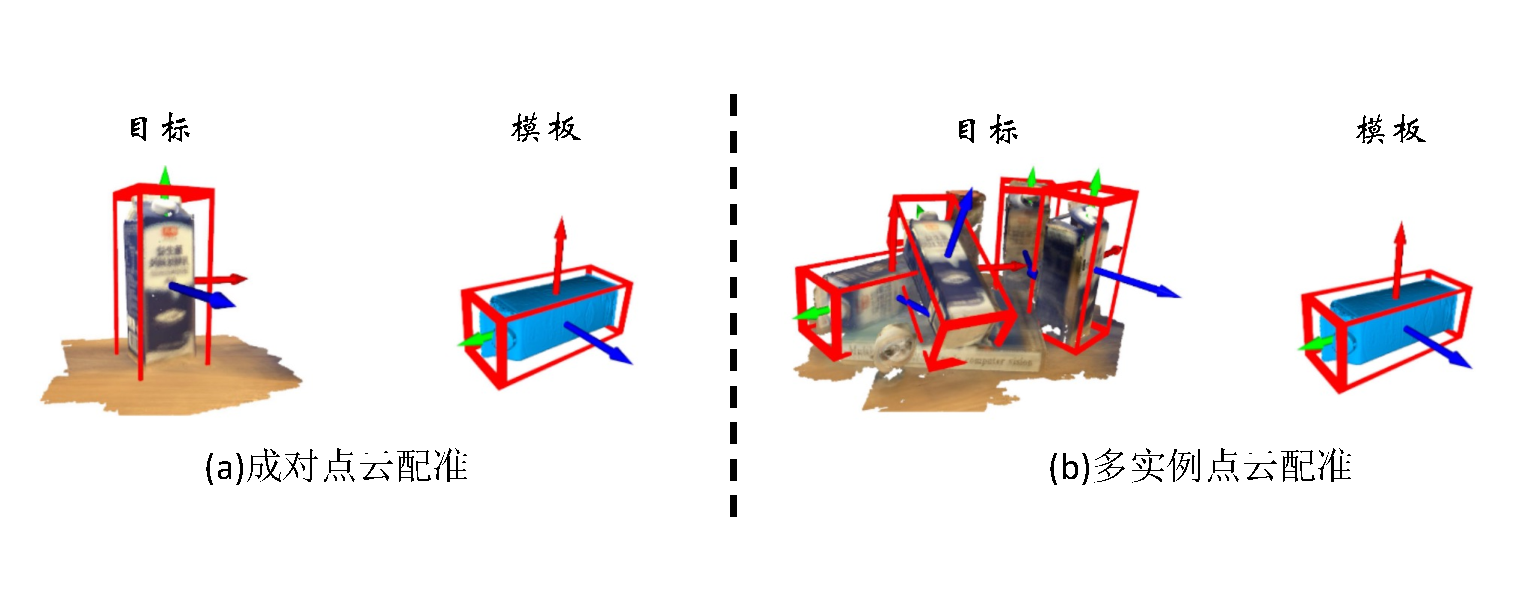
\includegraphics[width=\textwidth]{images/teaser.pdf}
    \caption{\textbf{多实例点云配准: } 给定目标的模板点云,成对点云配准(左)侧重于估计模板点云和目标点云之间的单个刚性变换,而多实例点云配准(右)旨在估计目标点云中相同物体的6D位姿。
    }
    \label{fig:teaser}
    \vspace{-10mm}
\end{figure*}

目前大多数点云配准任务研究主要集中在成对配准上。然而,在实际应用中,目标场景可能包含多个重复实例,我们需要估计模板点云与目标点云中这些重复实例之间的多个刚性变换。比如说在室内场景中,我们希望机器人能够将屋子中所有的椅子摆正,那么首先需要将多个椅子点云和模板椅子点云进行配准,求的目标椅子的位姿,通过机械运动来达到位姿改变的效果。图 \ref{fig:teaser} 展示了了一个示例。这个问题被命名为多实例点云配准,它比成对点云配准更具挑战性。针对该任务已有的现有文献研究较少,扩展现有的点云配准方法来解决这个问题并非易事。多实例点云配准不仅需要从嘈杂的对应中拒绝异常值,还需要识别单个实例的异常值集,这使得它比传统的配准问题更具挑战性。

与传统的两两配准方法相比,多实例点云配准需要解决更复杂的问题,同时也具有更广泛的应用价值。比如,在大规模场景重建任务中,通常需要处理成千上万个点云数据。单纯采用两两配准的方法可能导致累积误差,从而影响重建结果的精度。因此,研究多实例点云配准算法具有重要的实际意义。在机械臂抓取任务中,多实例点云配准算法可以在全局范围内考虑点云之间的约束关系,有助于消除局部误差和噪声的影响,从而提高配准结果的鲁棒性 \cite{stuckler2012robust} 。

尽管多实例点云配准技术在近年来取得了显著的进展,仍然存在许多亟待解决的问题。例如,现存的多实例点云配准一般采用多任务的方式,也就是先对点云分割或者三维目标检测,然后进行两两点云配准,这样的方式需要先训练点云分割或者目标检测网络,泛化性差。并且如果见到了不存在先验的点云,下游的配准任务仍然会失效。所以,本文我们会对多实例点云配准进行研究,通过点云直接进行多实例点云配准,不需要先进行点云分割或者目标检测,从而提高多实例点云配准的泛化性。


\section{国内外研究现状}

\subsection{点云配准}
点云配准长期以来一直是计算机视觉和机器人领域的一项基本任务,大致可分为直接方法 \cite{besl1992method, pomerleau2015review} 和基于特征的方法 \cite{qi2017pointnet,huang2021predator,bai2021pointdsc} 。近年来,由于深度学习的发展,许多基于特征的方法取得了最先进的性能。这些方法通常通过特征匹配产生对应关系,然后移除异常值以稳健地估计转换。尽管深度特征 \cite{qi2017pointnet,huang2021predator,bai2021pointdsc, wang2022you} 发展迅速,但特征匹配生成的对应关系仍然包含异常值。因此,去除异常点在点云配准中具有重要意义。过去,已经提出了许多传统方法来去除异常值,包括基于RANSAC的方法 \cite{barath2021progressive,zhao2021progressive,barath2018graph} 、基于分支和边界的方法 \cite{kluger2020consac} 以及许多其他方法 \cite{huang2021predator,yang2020teaser} 。最近,一系列基于学习的方法 \cite{bai2020d3feat,yi2018learning} 被提出,并在异常值去除方面取得了显着的效果。
以上的方法都是基于成对点云配准来完成的。然而,与成对配准不同,一个实例的内点构成多实例点云配准中所有其他实例的异常值。这种伪异常值使得很难将上述二元分类模型直接推广到多实例点云配准的情况。
现有该问题解决方案包括采用目标检测方法或对目标点云应用实例分割,将多实例点云配准问题转化为多个成对点云配准问题,但是这种方法需要预先训练一个目标检测或者点云分割网络,这样的方法对于已有点云类别是有效的,但是对于未知的类别是不适用的。另一种解决方案是通过多模型拟合,但是现有的多模型拟合方法依赖于抽样有效假设,当模型数量或离群率变高时,会涉及大量的抽样步骤,使得这些算法的效率和鲁棒性急剧下降。

\subsection{三维目标检测和实例分割}
三维物体的目标检测和实例分割与多实例点云配准有着密切的关系。输入一帧点云,目标检测模型 \cite{qi2019deep} 可以用来对获取每个目标对象的边界框,三维实例分割 \cite{wang2018sgpn,han2020occuseg} 为每个点生成实例标签。

这样的方法产生的结果类似于多实例点云配准的结果,但是它们需要将特定对象或类别的先验训练到网络中。基于点云匹配的筛选和聚类方法来进行多实例点云配准通过直接将模板点云和目标点云中的多个实例对齐来处理两组点云,而不使用任何关于输入的点云的先验信息。

\subsection{多模型拟合}
多实例配准也可以通过多模型拟合来实现,其目的是根据多个模型生成的数据点来进行建模。例如在点云中拟合多个平面 \cite{barath2018multi} ,在运动分割中估计基本矩阵 \cite{hartley1997defense} ,在多实例点云配准中计算刚性变换 \cite{tang2022multi} 等。但是由于一个实例的正常值构成所有其他实例的离群值,所以多模型拟合比单模型拟合更具挑战性。

现有的多模型拟合方法大致可以分为两类。第一类按顺序拟合模型 \cite{barath2019progressive,barath2021progressive,kanazawa2004detection,kluger2020consac} ,通过重复采样和筛选模型来进行建模。比如,Progressive-X \cite{barath2019progressive} 和Progressive-X+ \cite{barath2021progressive} 使用了表现更好的Graph-cut RANSAC \cite{barath2018graph} 作为采样方法来生成假设。CONSAC \cite{kluger2020consac} 首次将深度模型引入多模型拟合中,使用类似PointNet \cite{qi2017pointnet} 的网络来引导采样。通过重复采样来恢复单个实例,从输入中删除正常值和,以顺序的方式来检测实例。

第二类模型同时拟合多个模型 \cite{tang2022multi,toldo2008robust,magri2016multiple,magri2014t,magri2015robust} 。许多基于偏好分析的方法 \cite{toldo2008robust,magri2015robust} 最初对一系列假设进行采样,然后根据假设的残差对输入点进行聚类。ECC \cite{tang2022multi} 利用点云刚性变换空间一致性 \cite{leordeanu2005spectral} 和以自下而上的方式基于距离不变矩阵对对应关系进行聚类。PointCLM \cite{yuan2022pointclm} 使用了一种新的深层表示方法来与空间一致性相结合,得到了更好的结果。

% 本项目希望基于旋转等变的描述子来实现性能的初步提升,希望在模型中加入更多的内在形状和几何信息。通过端到端的方法优化整个方法系统,实现更高的准确性和鲁棒性。
\section{论文结构安排}
本论文共分为6章。

第一章为绪论,本章主要阐述了三维点云配准研究的重要性、背景以及现有的研究进展。通过对国内外三维点云配准研究文献的梳理和调查,我们对该领域的发展轨迹和现状进行了总结,并分析了先前研究所展现出的优点与缺点。同时,我们也详细介绍了本研究所完成的主要任务和做出的关键贡献。考虑到过去的研究中仍存在未完全解决的问题和挑战,我们特别指出了本研究所应用的策略和解决方案。最后,我们规划了清晰的文章结构,以引导读者理解本研究的整体框架。

在第二章,我们主要阐述了三维点云的基本数据格式和在本研究中所涉及的基础数学知识。同时,我们对在本研究中所用到的关于三维刚体变换的基础知识进行了详尽的总结和描述。

第三章在介绍了主要的数据集和评价指标后,引出深度学习方法在三维点云配准领域的研究与应用,并结合深度学习在三维点云配准领域做出的代表性工作 PointNet \cite{qi2017pointnet} 和 PointNet++ \cite{qi2017pointnet++} 进行介绍,并介绍和使用 PREDATOR \cite{huang2021predator} 作为骨干网络提取点云的点对特征供后续使用。

第四章主要介绍了本文提出的多实例点云配准,首先我们根据点云的特征进行聚类,然后对每个聚类进行对应聚类,最后进行刚性变换估计;其次,我们引入深度学习的方法,学习鲁棒的点对特征,进行谱聚类,得到了点云配准更好的效果和更高的指标。

第五章主要介绍了本文的实验结果,包括多实例点云配准的定性和定量实验,证明了本文提出的方法的有效性和鲁棒性。
\section{小结}
本章主要介绍了点云配准任务以及多实例点云配准任务的研究背景和研究意义、国内外研究现状。然后介绍了本文的研究内容和结构安排。

% 在这里添加第二章、第三章……TeX 文件的引用
%%
% The BIThesis Template for Bachelor Graduation Thesis
%
% 北京理工大学毕业设计 (论文) 第二章节 —— 使用 XeLaTeX 编译
%
% Copyright 2020-2023 BITNP
%
% This work may be distributed and/or modified under the
% conditions of the LaTeX Project Public License, either version 1.3
% of this license or (at your option) any later version.
% The latest version of this license is in
%   http://www.latex-project.org/lppl.txt
% and version 1.3 or later is part of all distributions of LaTeX
% version 2005/12/01 or later.
%
% This work has the LPPL maintenance status `maintained'.
%
% The Current Maintainer of this work is Feng Kaiyu.
%%

\chapter{点云配准相关背景知识介绍}
本章将对点云配准的基本理论和相关背景知识进行系统阐述,首先会介绍点云数据的特征,然后会对点云配准的刚体运动和运动参数估计进行介绍。

\section{点云数据}
三维世界中的数据表证有多种类型,如点云数据 (Point Clouds) \cite{leberl2010point} 、三角网格 (Triangle Mesh) \cite{jiang2020local} 、体素 (Voxel Grids) \cite{guan2020voxel} 、深度相机数据 (RGB-D Camera) \cite{cruz2012kinect} 等,可视化数据如图 \ref{fig:3ddata} 所示,本文主要研究的是点云数据,因此本节将对点云数据进行简要介绍。

\begin{figure*}[ht]
    \vspace{-8mm}
    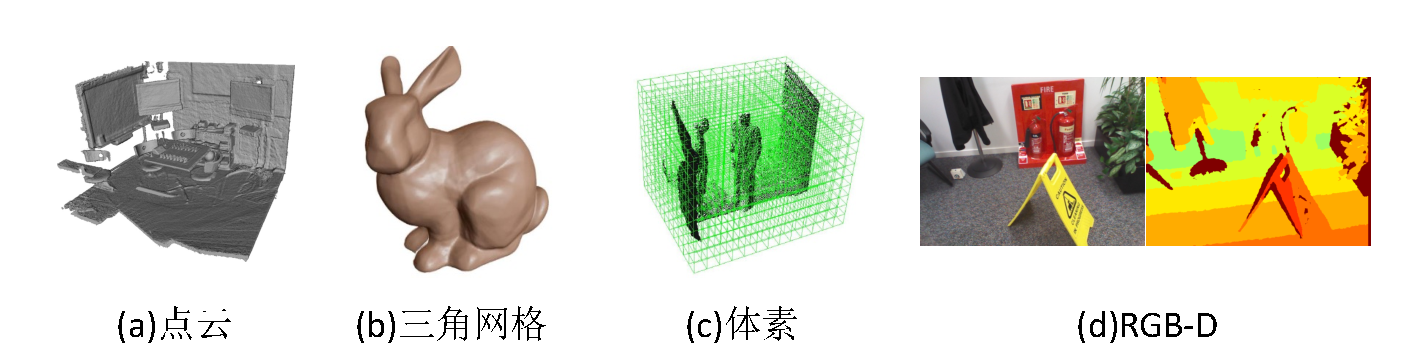
\includegraphics[width=\textwidth]{images/3ddata.pdf}
    \caption{点云、三角网格、体素、深度相机数据可视化示意图}
    \label{fig:3ddata}
    \vspace{-10mm}
\end{figure*}


\subsection{点云数据特点}
点云数据是一种常用的三维数据表征形式,由一系列具有三维坐标 (X, Y, Z) 的点组成。这些点可以通过激光雷达、结构光传感器、多视角立体视觉等方式采集。点云数据具有以下特点:

1. 无序性:点云数据通常是无序的,即点在数据结构中的顺序并不表示它们在空间中的相对位置。这使得处理点云数据时需要额外关注邻域搜索等问题。

2. 不完整性:由于采集设备的视野限制以及物体遮挡等因素,点云数据往往只能捕捉到物体表面的部分信息,无法完整地描述物体的几何结构。

3. 稀疏性:点云数据在空间中分布可能是不均匀的,有些区域可能点密集,而有些区域可能点稀疏。这会对点云处理算法的性能产生影响。

4. 噪声敏感性:点云数据容易受到测量噪声、环境光照等因素的影响。为了提高数据质量,通常需要对点云进行预处理,如滤波、降采样等。

5. 缺乏拓扑信息:点云数据仅包含物体表面的几何信息,不包含拓扑信息。在需要考虑物体结构的应用场景中,点云数据需要进行进一步处理,如重建三角网格或提取骨架结构等。

6. 可扩展性:点云数据可以方便地扩展以包含其他属性信息,如颜色、法向量、强度等。这有助于提高点云处理算法的性能和鲁棒性。

7. 易于处理和存储:由于点云数据直接表示了物体表面的几何信息,其数据结构简单,便于处理和存储。此外,点云数据可以通过各种数据结构 (如KD树、八叉树等) 进行高效的组织和检索。

在应用深度学习算法时,由于点云数据的无序性,深度学习算法,比如全连接层、卷积层等无法直接应用于点云数据。因此,需要对点云数据进行预处理,将其转换为有序的数据表征形式,如三角网格\cite{jiang2020local}、体素\cite{guan2020voxel}等。但是这样的方法会造成空间中很多点的浪费,使得输入的数据变得更加稀疏,使得训练数据变少。PointNet\cite{qi2017pointnet}是一种用于处理点云数据的深度学习网络结构,于2017年首次提出。它是一个端到端的神经网络,可以直接从原始点云数据中学习特征表示。PointNet通过使用对称函数 (如最大池化) 处理输入点云的无序性,同时具有对输入点顺序的不变性。


\subsection{点云特征描述}
三维点云的特征描述,也叫描述子(Descriptor),是一种用于表示点云数据中每个点周围的局部几何特征的向量。描述子捕捉了点云中每个点的几何结构和形状信息,这对于解决诸如点云配准、物体识别、分类和分割等问题至关重要。点云描述子应具有以下特性:鲁棒性、区分性、旋转不变性、尺度不变性和噪声不敏感性。点云描述子对于点云的后处理有着非常巨大的影响,对于不同的任务和数据特征,应该选用合适的描述子来作为网络的预处理。

有许多不同类型的点云描述子,它们根据计算方法和考虑的几何属性而有所不同。以下是一些常见的点云描述子:

1. Spin Images (旋转图像)  \cite{johnson1997spin} :通过在点云中每个点周围投影二维图像来表示局部形状信息。

2. Normal Aligned Radial Features (NARF)  \cite{steder2010narf} :基于局部表面法线的方向和强度来描述点云中的局部特征。

3. Fast Point Feature Histograms (FPFH)  \cite{rusu2009fast} :通过计算每个点周围的点对的几何特征直方图来表示局部特征。

4. Signature of Histograms of Orientations (SHOT)  \cite{salti2014shot} :结合局部点的颜色信息和表面法线分布,为每个点计算描述子。

5. Point Pair Features (PPF)  \cite{deng2018ppfnet} :描述点云中两个点之间的几何关系,PPF 是一个四元组$(\alpha, d, \theta, \phi)$,其中$\alpha$是两点之间的距离,$d$是两点的法向量之差,$\theta$是两点的法线之间的角度,$\phi$是两点的法线在两点之间连线所确定的平面上的角度。PPF特征在处理点云配准问题时具有很高的鲁棒性,因为它仅依赖于点云的几何信息。

\section{刚体运动表示}
刚体运动表示是点云配准任务的最后一个阶段的任务。对于位移来说,常用的是位移向量 (Transition) ;旋转的运动参数有不同的表示形式,如欧拉角\cite{pio1966euler} 、四元数\cite{shoemake1985animating} 、旋转矩阵\cite{horn1954doubly} 、轴角\cite{diebel2006representing} 等。下面本文进行简要介绍。

\subsection{旋转矩阵}
旋转矩阵是一种与向量相乘时旋转向量同时保持其长度的矩阵。所有 $3 \times 3$ 旋转矩阵的特殊正交群表示为 $SO(3)$。因此,如果 $\boldsymbol{R} \in SO(3)$,那么
\begin{equation}
\det (\boldsymbol{R}) = \pm1 \quad \text{且} \quad \boldsymbol{R}^{-1} = \boldsymbol{R}^T
\end{equation}

对于满足 $\det (\boldsymbol{R}) = 1$ 的旋转矩阵,称为正规旋转;对于满足 $\det (\boldsymbol{R}) = -1$ 的旋转矩阵,称为非正规旋转。非正规旋转也称为旋转倒数,由旋转后接反演操作组成。本文将分析限制在正规旋转上,因为非正规旋转不是刚体变换。
本文按如下方式引用旋转矩阵的元素:
\begin{align}
    \boldsymbol{R} &=
    \begin{bmatrix}
    r_1 & r_2 & r_3
    \end{bmatrix} \\
    &=
    \begin{bmatrix}
    r_{11} & r_{12} & r_{13} \\
    r_{21} & r_{22} & r_{23} \\
    r_{31} & r_{32} & r_{33}
    \end{bmatrix}
\end{align}

对于旋转矩阵,本文可以使用群的定义来进行更精准的定义。
\begin{equation}
    SO(n) = \{\boldsymbol{R} \in \mathbb{R}^{n \times n} | \boldsymbol{R}^T\boldsymbol{R} = \boldsymbol{I}, \det (\boldsymbol{R}) = 1\}
\end{equation}
其中,$SO(n)$是特殊正交群 (Special Orthogonal Group),这个集合由$n$维空间的旋转矩阵组成。$SO(n)$是一个群,因为它满足群的四个条件:封闭性、结合律、单位元和逆元。$SO(n)$的单位元是 $\boldsymbol{I}$,逆元是 $\boldsymbol{R}^T$。$SO(n)$的元素称为正规旋转矩阵。通过旋转矩阵可以直接描述相机的旋转。

为了描述两个坐标之间的相对旋转,本文假设某个单位正交基 $\boldsymbol{i}, \boldsymbol{j}, \boldsymbol{k}$,并且本文希望将其旋转到另一个正交基 $\boldsymbol{i}', \boldsymbol{j}', \boldsymbol{k}'$。假设对于同一个向量$\boldsymbol{a} = [a_1, a_2, a_3]^T$,在两个坐标系中的表示分别为 $\boldsymbol{a} = a_1\boldsymbol{i} + a_2\boldsymbol{j} + a_3\boldsymbol{k}$ 和 $\boldsymbol{a}' = a_1'\boldsymbol{i}' + a_2'\boldsymbol{j}' + a_3'\boldsymbol{k}'$,根据坐标的定义,有
\begin{equation}
    [\boldsymbol{i}, \boldsymbol{j}, \boldsymbol{k}] \boldsymbol{a} = [\boldsymbol{i}', \boldsymbol{j}', \boldsymbol{k}'] \boldsymbol{a}'
\end{equation}
本文对上述等式同时左成$[\boldsymbol{i}, \boldsymbol{j}, \boldsymbol{k}]^T$,本文可以通过旋转矩阵 $\boldsymbol{R}$ 来表示两个坐标系之间的旋转关系,即
\begin{equation}
    \boldsymbol{a}' = 
    \begin{bmatrix}
    \boldsymbol{i}^T \boldsymbol{i}' & \boldsymbol{i}^T \boldsymbol{j}' & \boldsymbol{i}^T \boldsymbol{k}' \\
    \boldsymbol{j}^T \boldsymbol{i}' & \boldsymbol{j}^T \boldsymbol{j}' & \boldsymbol{j}^T \boldsymbol{k}' \\
    \boldsymbol{k}^T \boldsymbol{i}' & \boldsymbol{k}^T \boldsymbol{j}' & \boldsymbol{k}^T \boldsymbol{k}'
    \end{bmatrix}
    =
    \boldsymbol{R} \boldsymbol{a}
\end{equation}

因为旋转矩阵是正交矩阵,它的逆就可以用来描述一个相反的旋转,按照上面的推到,则有:
\begin{equation}
    \boldsymbol{a} = \boldsymbol{R}^T \boldsymbol{a}' = \boldsymbol{R}^{-1} \boldsymbol{a}'
\end{equation}

在欧式变换中,除了旋转还有平移,将$\boldsymbol{a}$经过一次旋转$\boldsymbol{R}$和平移$\boldsymbol{t}$,最终得到了$\boldsymbol{a}'$,把旋转和平移组合起来,得到:
\begin{equation}
    \boldsymbol{a}' = \boldsymbol{R} \boldsymbol{a} + \boldsymbol{t}
    \label{eq:rotation_translation}
\end{equation}

\subsection{变换矩阵}
在三维空间中,本文可以通过平移和旋转来描述一个刚体的变换。本文将平移和旋转组合起来,得到一个变换矩阵,用来描述一个刚体的变换。假设本文有一个刚体,它的初始位置在原点,本文将它平移到 $\boldsymbol{t}$,然后将它旋转到 $\boldsymbol{R}$,则这个刚体的变换矩阵为:
\begin{equation}
    \boldsymbol{T} = 
    \begin{bmatrix}
    \boldsymbol{R} & \boldsymbol{t} \\
    \boldsymbol{0}^T & 1
    \end{bmatrix}
\end{equation}
将向量改写为齐次形式$\widetilde{\boldsymbol{a}} = [a_1, a_2, a_3, 1]^T = [\boldsymbol{a}, 1]^T$, 那么本文可以将式 \ref{eq:rotation_translation} 重写为:
\begin{equation}
    \widetilde{\boldsymbol{a}}' = \boldsymbol{T} \widetilde{\boldsymbol{a}} = \boldsymbol{R} \boldsymbol{a} + \boldsymbol{t}
\end{equation}  

依靠变换矩阵,本文可以对多次变换的累加进行很简洁的数学表达。假设本文有一个刚体$\boldsymbol{a}$,它的初始位置在原点,本文将它经过 $\boldsymbol{T}_1, \boldsymbol{T}_2$ 两次变换,则这个刚体的最终位置为$\widetilde{\boldsymbol{a}}' = \boldsymbol{T}_1 \boldsymbol{T}_2 \widetilde{\boldsymbol{a}}$。

\subsection{欧拉角}
三次坐标旋转依次可以描述任意旋转。本文考虑三次旋转,其中第一次旋转是关于 $x$ 轴的角度 $\psi$,第二次旋转是关于 $y$ 轴的角度 $\theta$,第三次旋转是关于 $z$ 轴的角度 $\phi$,如图 \ref{fig:rotation} (a, b ,c)所示。为了简化符号,本文将这些角度排列成一个三维向量,称为欧拉角向量,定义为 
\begin{equation}
    \boldsymbol{u} := [\phi, \theta, \psi]^\text{T}
\end{equation}
将欧拉角向量映射到其对应的旋转矩阵的函数,$\boldsymbol{R}_{ijk} : \mathbb{R}^3 \to SO(3)$,定义为
\begin{equation}
    \boldsymbol{R}_{ijk}(\phi, \theta, \psi) := \boldsymbol{R}_i(\phi)\boldsymbol{R}_j(\theta)\boldsymbol{R}_k(\psi)
\end{equation}
与一般情况相同,如果 $\boldsymbol{z} \in \mathbb{R}^3$ 是世界坐标系中的一个向量,$\boldsymbol{z}_0 \in \mathbb{R}^3$ 是以体固定坐标表示的相同向量,那么以下关系成立:
\begin{align}
    \boldsymbol{z}_0 = \boldsymbol{R}_{ijk}(\boldsymbol{u}) \boldsymbol{z} \\
    \boldsymbol{z} = \boldsymbol{R}_{ijk}(\boldsymbol{u})^T \boldsymbol{z}_0
\end{align}
也就是说,欧拉角并不是定义在三维线性空间的群,欧拉角的相互转换需要借助旋转矩阵来进行表达。

\begin{figure}
    \centering
    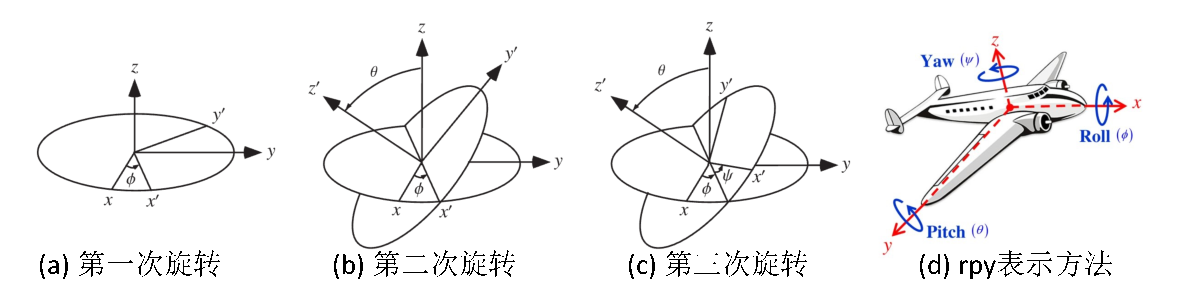
\includegraphics[width=\textwidth]{images/rotation.pdf}
    \caption{欧拉角旋转表示}
    \label{fig:rotation}
    \vspace{-0.5cm}
\end{figure}

在自动化或者航空航天领域比较常用的欧拉角的分解方式是 $Z-Y-X$,也就是说,先绕 $z$ 轴旋转 $\psi$ 角,然后绕 $y$ 轴旋转 $\theta$ 角,最后绕 $x$ 轴旋转 $\phi$ 角。这种分解方式也被称为航空分解 (Aerospace decomposition) ,通常这种方式中的$Z-Y-X$会被称为“偏航 - 俯仰 - 旋转 (yaw - pitch - roll)”。在这种分解方式中,欧拉角向量的顺序是 $\boldsymbol{u} = [\psi, \theta, \phi]^\text{T}$,如图 \ref{fig:rotation} (d)所示。

欧拉角的一个缺点是会碰到著名的万象锁问题\cite{vsenk2006rotation} ,也就是说,当 $\theta = \pm \frac{\pi}{2}$ 时,旋转矩阵 $\boldsymbol{R}_{ijk}(\boldsymbol{u})$ 的值会变成奇异的。理论上可以证明,只要想要用3个数来表达三位旋转时,基本都会碰到奇异性问题\cite{stuelpnagel1964parametrization} 。由于这种原理,欧拉角不适用于迭代和插值,在传统的SLAM中和深度学习中几乎都不会是用这种方式来进行迭代,但是欧拉角对于人机交互是友好的。

\subsection{四元数}
旋转矩阵使用了9个未知数来描述3自由度的旋转,这在数学表达上具有冗余性了;欧拉角使用了3个未知数来描述3自由度的旋转,在数学表达上是紧凑的,但是具有奇异性。因为本文找不到不带奇异性,且使用3个未知数的方法来描述3维旋转的描述方式\cite{stuelpnagel1964parametrization} 。这个性质,可以类比于用两个坐标描述地球表面 (二维流形) 上的点,本文可以使用经纬度来描述地球表面上的点,但是在极点处,经纬度的表达就会出现奇异性,即纬度为$\pm 90^{\circ}$时,经度无意义。

三位旋转是一个三维流形,因此,为了最优平衡无奇异性和数学表达的紧凑性,本文需要引入一个新的数学工具来描述3自由度的旋转,这个数学工具就是四元数。四元数是Hamilton找到的一种超复数,它在数学形式上既是紧凑的,又是非奇异的。四元数的定义如下:
\begin{equation}
    \boldsymbol{q} = q_0 + q_1 i + q_2 j + q_3 k
\end{equation}
其中,$q_0, q_1, q_2, q_3 \in \mathbb{R}$,$i, j, k$ 是四元数的三个虚数单位,满足如下关系:
\begin{equation}
    \left\{
    \begin{aligned}
        &i^2 = j^2 = k^2 = ijk = -1, \\
        &ij = k, jk = i, ki = j, \\
        &ji = -k, kj = -i, ik = -j
    \end{aligned}
    \right.
\end{equation}
假设某个旋转是绕着单位向量 $\boldsymbol{u} = [u_x, u_y, u_z]^T$ 旋转 $\theta$ 角,那么这个旋转可以用四元数来表示为:
\begin{equation}
    \boldsymbol{q} = \cos \frac{\theta}{2} + \sin \frac{\theta}{2} (u_x i + u_y j + u_z k)
\end{equation}
同时,本文也可以从单位四元数种计算出对应的旋转轴和旋转角:
\begin{equation}
    \left\{
    \begin{aligned}
        &\theta = 2 \arccos q_0, \\
        &u_x = \frac{q_1}{\sin \frac{\theta}{2}}, u_y = \frac{q_2}{\sin \frac{\theta}{2}}, u_z = \frac{q_3}{\sin \frac{\theta}{2}}
    \end{aligned}
    \right.
\end{equation}

因为四元数是定义在复向量空间中而非旋转流形中,并且四元数没有死锁的特性,所以在深度学习的梯度下降算法中,常常用四元数作为回归的目标。并且,因为三维流形的性质,本文在四元数中同乘一个常数,可以得到相同的旋转,即$[q_0, q_1, q_2, q_3] \iff k[q_0, q_1, q_2, q_3]$。由于这个性质,在回归任务中,本文通常回归单位四元数,即$\sum_0^3 q_i^2 = 1$。

{\bf 用四元数表示旋转。} 用四元数同样也可以表达对一个点的旋转,假设一个空间中的三维坐标点为$\boldsymbol{a} = [x, y, z] \in \mathbb{R}^3$。以及一个旋转轴$\boldsymbol{n}$和旋转角$\theta$,这个点绕着旋转轴旋转$\theta$角后的坐标为$\boldsymbol{a}'$,则:
\begin{equation}
    \boldsymbol{p}' = \boldsymbol{Rp} = \boldsymbol{qpq}^{-1}
\end{equation}
其中,$\boldsymbol{q} = [\cos \frac{\theta}{2}, \boldsymbol{n} \sin \frac{\theta}{2}]$。


\section{运动学参数估计}
\subsection{基于奇异值分解的线性代数求解}
奇异值分解\cite{levinson2020analysis} (Singular Value Decomposition, SVD) 是线性代数中一种重要的矩阵分解,在信号处理、计算机视觉、运动估计中有着非常广泛的运用。下面,本文对奇异值分解的线性代数部分进行简要介绍。

奇异值分解对一个矩形数据矩阵 (定义为$\boldsymbol{A}$,其中$\boldsymbol{A}$是一个$n \times p$矩阵) 进行处理,其中n行代表观察值,p列代表变量。SVD定理如下:
\begin{equation}
\boldsymbol{A}_{n \times p} = \boldsymbol{U}_{n \times n} \boldsymbol{S}_{n \times p} \boldsymbol{V}^T_{p \times p}
\end{equation}
其中
\begin{align}
    \boldsymbol{U}^T \boldsymbol{U} = \boldsymbol{I}_{n \times n} \\
    \boldsymbol{V}^T \boldsymbol{V} = \boldsymbol{I}_{p \times p}
\end{align}

即$\boldsymbol{U}$和$\boldsymbol{V}$是正交的。$\boldsymbol{U}$的列是左奇异向量 (观察值系数向量) ;$\boldsymbol{S}$ (与$\boldsymbol{A}$的维度相同) 具有奇异值,并且是对角的 (模振幅) ;$\boldsymbol{V}^T$的行是右奇异向量 (变量水平向量)。SVD表示了原始数据在协方差矩阵为对角线的坐标系中的扩展。

计算SVD包括寻找$\boldsymbol{A} \boldsymbol{A}^T$和$\boldsymbol{A}^T \boldsymbol{A}$的特征值和特征向量。$\boldsymbol{A}^T \boldsymbol{A}$的特征向量构成$\boldsymbol{V}$的列,$\boldsymbol{A} \boldsymbol{A}^T$的特征向量构成$\boldsymbol{U}$的列。此外,$\boldsymbol{S}$中的奇异值是来自$\boldsymbol{A} \boldsymbol{A}^T$或$\boldsymbol{A}^T \boldsymbol{A}$的特征值的平方根。奇异值是$\boldsymbol{S}$矩阵的对角线条目,并按降序排列。奇异值总是实数。如果矩阵$\boldsymbol{A}$是实数矩阵,那么$\boldsymbol{U}$和$\boldsymbol{V}$也是实数。

奇异值分解 (SVD) 在点云配准问题中也具有重要应用。点云配准是将两个或多个点云数据集合并为一个统一坐标系的过程。在这种情况下,本文的目标是找到一个最优的刚体变换,包括旋转和平移,使得两个点云之间的距离最小化。

假设本文有两个点云数据集$\boldsymbol{P}$和$\boldsymbol{Q}$,每个点云包含$n$个点。本文首先计算两个点云的质心$\boldsymbol{p}_c$和$\boldsymbol{q}_c$,然后将点云平移到原点。接下来,本文计算点云$\boldsymbol{P}$和$\boldsymbol{Q}$之间的距离矩阵$\boldsymbol{H}$,其中$\boldsymbol{H}=\boldsymbol{P}^T\boldsymbol{Q}$。

在这种情况下,本文可以使用SVD来求解最优的旋转矩阵$\boldsymbol{R}$,使得两个点云之间的距离最小化。具体来说,本文对距离矩阵$\boldsymbol{H}$进行奇异值分解:

\begin{equation}
\boldsymbol{H} = \boldsymbol{U} \boldsymbol{S} \boldsymbol{V}^T
\end{equation}

然后,本文计算旋转矩阵$\boldsymbol{R}$:

\begin{equation}
\boldsymbol{R} = \boldsymbol{U} \boldsymbol{V}^T
\end{equation}

如果$\boldsymbol{R}$是一个不合适的旋转矩阵 (即$\det(\boldsymbol{R})\neq 1$) ,本文可以通过修改$\boldsymbol{S}$矩阵来修复它。具体而言,本文将$\boldsymbol{S}$的最小奇异值设为$-1$,然后重新计算旋转矩阵$\boldsymbol{R}$。

最后,本文可以计算最优的平移向量$\boldsymbol{t}$:

\begin{equation}
\boldsymbol{t} = \boldsymbol{q}_c - \boldsymbol{R} \boldsymbol{p}_c
\end{equation}

通过应用旋转矩阵$\boldsymbol{R}$和平移向量$\boldsymbol{t}$,本文可以将点云$\boldsymbol{P}$对齐到点云$\boldsymbol{Q}$,从而实现点云配准。

\subsection{基于Levenberg-Marquardt算法的非线性优化求解}
在数学和计算领域,Levenberg-Marquardt算法 (LMA或简称LM) \cite{levenberg1944method} ,也称为阻尼最小二乘法 (DLS) ,用于求解非线性最小二乘问题。这些最小化问题尤其出现在最小二乘曲线拟合中。LMA在高斯-牛顿算法 (GNA) 和梯度下降法之间进行插值。LMA比GNA更稳健,这意味着在许多情况下,即使它从距离最终最小值非常远的地方开始,也能找到解决方案。对于行为良好的函数和合理的初始参数,LMA往往比GNA慢。LMA也可以被视为使用信任区域方法的高斯-牛顿算法。

需要LM算法求解的问题被称为非线性最小二乘最小化问题。这意味着要最小化的函数具有以下特殊形式:

\begin{equation}
f(x) = \frac{1}{2} \sum_{j=1}^{m} r_j^2(x)
\end{equation}

其中 $x = (x_1, x_2, \dots, x_n)^T$ 是一个向量,每个 $r_j$ 是一个从 $\mathbb{R}^n$ 到 $\mathbb{R}$ 的函数。$r_j$ 被称为残差,并且假定 $m \geq n$。

为了简化问题,本文用残差向量 $r : \mathbb{R}^n \rightarrow \mathbb{R}^m$ 来表示 $f$,定义为:

\begin{equation}
r(x) =
\begin{bmatrix}
r_1(x) \
r_2(x) \
\cdots \
r_m(x)
\end{bmatrix}
\end{equation}

现在,$f$ 可以重写为 $f(x) = \frac{1}{2} ||r(x)||^2$。$f$ 的导数可以用相对于 $x$ 的 $r$ 的雅可比矩阵 $J(x)$ 来表示,定义为 $J(x) = \frac{\partial r_j}{\partial x_i}$,其中 $1 \leq j \leq m$,$1 \leq i \leq n$。

首先考虑线性情况,其中每个 $r_i$ 函数都是线性的。在这里,雅可比矩阵是常数,本文可以将 $r$ 表示为空间中的超平面,这样 $f$ 给出二次型:

\begin{equation}
f(x) = \frac{1}{2} ||Jx - r_0||^2
\end{equation}

本文还得到 $\nabla f(x) = J^T(Jx - r_0)$ 和 $\nabla^2 f(x) = J^TJ$。通过将 $\nabla f(x) = 0$ 求解最小值,本文得到 $x_\text{min} = (J^TJ)^{-1}J^Tr$,这是一组无约束优化问题的解。

回到一般的非线性情况,本文有:

\begin{equation}
\nabla f(x) = J(x)^T r(x)
\label{eq:grad}
\end{equation}

\begin{equation}
\nabla^2 f(x) = J(x)^TJ(x) + \sum_{j=1}^{m} r_j(x) \nabla^2 r_j(x)
\label{eq:hessian}
\end{equation}

最小二乘问题的独特属性是,给定雅可比矩阵 $J$,如果可以将 $r_j$ 用线性函数近似 ($\nabla^2 r_j(x)$ 较小) 或残差 $r_j(x)$ 本身较小,本文可以直接获得 Hessian 矩阵 ($\nabla^2 f(x)$) 。在这种情况下,Hessian 矩阵简化为:

\begin{equation}
\nabla^2 f(x) = J(x)^T J(x)
\label{eq:hessian_approx}
\end{equation}

这与线性情况相同。这里通常使用的近似是在解附近的 $r_i$ 近似线性,这样 $\nabla^2 r_j(x)$ 较小。还要注意,只有在残差较小时,式 \ref{eq:hessian_approx} 才有效。对于大残差问题,不能使用二次近似求解\cite{李娇娇2022基于深度学习的} 。

考虑到点云配准问题,本文可以将 Levenberg-Marquardt 算法应用于点云之间的非线性最小二乘优化问题。在这种情况下,本文寻求点云对应度量的最小距离,同时考虑旋转和平移变换。通过迭代地优化变换参数,Levenberg-Marquardt 算法可以在点云配准问题中找到一个稳定的解决方案。点云对应度量之间的误差主要有点到点 (point-to-point) 、点到面 (point-to-plane) 、面到面 (plane-to-plane) 这几类方式。如图 \ref{fig:point2plane} 所示,本文以最小化点到面距离为例,来说明 Levenberg-Marquardt 算法的求解过程。

\begin{figure}[htbp]
    \centering
    \vspace{-0.5cm}
    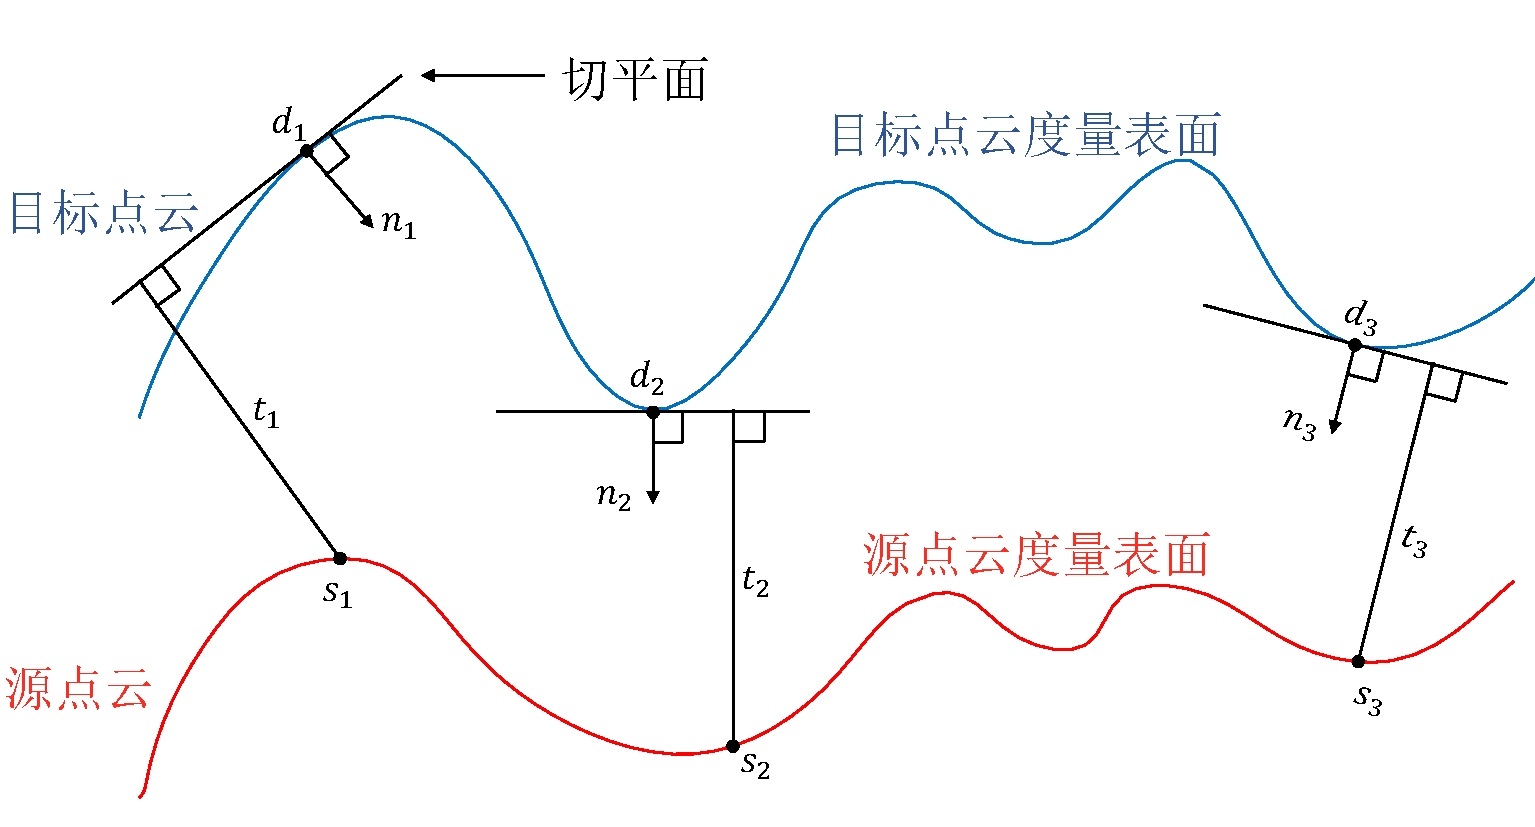
\includegraphics[width=0.8\textwidth]{images/LM_point2plane.pdf}
    \caption{最小化点到面距离示意图}
    \label{fig:point2plane} 
    \vspace{-1.5cm}
\end{figure}

在刚体运动参数估计任务中,LM 算法的关键步骤包括:

 (1) 在运动前的点云数据中找到特征点 $\boldsymbol{p}_i$ 和运动后的点云数据中对应的特征点 $\boldsymbol{q}_j$ 以及特征面 $\boldsymbol{S}_l$;

 (2) 计算特征点 $\boldsymbol{p}_i$ 到特征面 $\boldsymbol{S}_l$ 的欧氏距离 $d_e$;

 (3) 基于特征点到特征面的距离度量,构建匹配对的约束关系:
\begin{equation}
f(\boldsymbol{p}_i, \boldsymbol{T}) = d_e
\end{equation}
其中,$\boldsymbol{T}$ 代表刚体运动变换参数。

利用 LM 非线性优化方法,估计位姿变换矩阵:
\begin{equation}
\hat{\boldsymbol{T}} = \boldsymbol{T} - (\boldsymbol{J}^T \boldsymbol{J} + \lambda \boldsymbol{I})^{-1} \boldsymbol{J}^T f
\label{eq:LM}
\end{equation}
通过链式法则计算雅可比矩阵 (Jacobian Matrix):
\begin{equation}
\boldsymbol{J} = \frac{\partial f}{\partial \boldsymbol{T}} = \frac{\partial f}{\partial \boldsymbol{p}_i} \frac{\partial \boldsymbol{p}_i}{\partial \boldsymbol{T}}
\end{equation}
将雅可比矩阵带入公式 \ref{eq:LM},可以求解刚体运动变换参数 $\boldsymbol{T}$。

 (4) 检查变换参数是否为最优估计,如果满足以下条件:
\begin{equation}
0 < \frac{f(\boldsymbol{p}_i, \hat{\boldsymbol{T}}) - f(\boldsymbol{p}_i, \boldsymbol{T})}{|f(\boldsymbol{p}_i, \boldsymbol{T})|} < T_d
\end{equation}
则当前变换参数为最优估计。否则,调整阻尼因子 $\lambda$,继续迭代求解最优变换参数。其中,$T_d$ 是距离阈值。

 (5) 将求解得到的最优变换参数应用于运动前的特征点 $\boldsymbol{p}_i$,得到 $\boldsymbol{q}'_j$,如果满足以下条件:
\begin{equation}
|\boldsymbol{p}_i - \boldsymbol{q}_j| > |\boldsymbol{p}_i - \boldsymbol{q}'_j|
\end{equation}
则认为 $\boldsymbol{q}_j$ 是点 $\boldsymbol{p}_i$ 的最佳匹配点。否则,减小阻尼因子 $\lambda$,继续迭代求解最优匹配点对。如果达到最大迭代次数仍未找到最优匹配点对,将点 $\boldsymbol{p}_i$ 视为噪点并从原始点云数据中剔除,继续处理其他特征点。

总之,使用 LM 算法进行点云配准的过程可以分为以下几个步骤:\\
1. 在运动前后的点云数据中提取特征点和特征面;\\
2. 计算特征点之间的欧氏距离并建立约束关系;\\
3. 使用 LM 算法进行非线性优化,求解刚体运动变换参数;\\
4. 根据求解结果判断当前变换参数是否为最优估计;如非最优,调整阻尼因子并继续迭代;\\
5. 应用求解得到的最优变换参数,寻找最佳匹配点对;\\
6. 若达到最大迭代次数仍未找到最优匹配点对,将当前特征点视为噪点并剔除,继续处理其他特征点。

\section{小结}
本章主要介绍了点云配准任务的基础知识,包括点云数据的特点,运动学表达和刚体运动参数估计方法。主要介绍了两种最常用的点云配准求解刚体运动最优变换参数的方法,一个是基于奇异值分解 (SVD) 的线性代数求解方法,一个是基于Levenberg-Marquardt算法的非线性优化求解。
\chapter{基于深度学习的点云配准}
本章将结合深度学习,对点云配准进行研究。首先介绍深度学习中点云配准常用的公开数据集,然后介绍点云配准的评价指标并推广到多实例点云配准,最后介绍点云配准相关的深度学习技术。

\section{标准数据集}
本节将介绍用于点云配准的标准数据集。在评估不同指标的性能时,我们需要用到不同的公开数据集。点云配准任务的数据集大致可以分为仿真数据集和真实数据集。仿真数据集中的物体对象是完整的三维模型,比如ModelNet40\cite{sunmodelnet40}。而真实数据集中,因为存在遮挡、测量误差、相干光干扰、背景影响等问题,往往会存在缺失、噪声、过密/稀疏等问题,比如Scan2CAD\cite{avetisyan2019scan2cad}和ShapeNet\cite{chang2015shapenet}。下表\ref{tab:PointCloudDatasets}列出了常用的点云配准数据集。
\begin{table}[h!]
    \centering
    \vspace{-1.0cm}
    \caption{常见的点云信息处理任务数据集列表}
    \label{tab:PointCloudDatasets}
    \resizebox{\textwidth}{!}{
    \begin{tabular}{|l|c|c|c|c|c|c|c|}
    \hline
    \textbf{数据集名称} & \textbf{年份} & \textbf{场景数量} & \textbf{类别数量} & \textbf{训练集} & \textbf{测试集} & \textbf{类型} & \textbf{数据结构} \\ \hline
    McGill Benchmark \cite{siddiqi2008retrieving} & 2008 & 456 & 19 & 304 & 152 & 仿真场景 & 三角网格 \\ \hline
    Sydney Urban Objects \cite{de2013unsupervised} & 2013 & 588 & 14 & - & - & 真实场景 & 点云 \\ \hline
    ModelNet10 \cite{wu20153d} & 2015 & 4899 & 10 & 3991 & 605 & 仿真场景 & 三角网格 \\ \hline
    ModelNet40 \cite{sunmodelnet40} & 2015 & 12311 & 40 & 9843 & 2468 & 仿真场景 & 三角网格 \\ \hline
    ShapeNet \cite{chang2015shapenet} & 2015 & 51190 & 55 & - & - & 仿真场景 & 三角网格 \\ \hline
    ScanNet \cite{dai2017scannet} & 2017 & 12283 & 17 & 9677 & 2606 & 真实场景 & RGB-D \\ \hline
    ScanObjectNN \cite{uy2019revisiting} & 2016 & 2902 & 15 & 2321 & 581 & 真实场景 & 三角网格 \\ \hline
    S3DIS \cite{armeni20163d} & 2017 & 271 & 13 & - & - & 真实场景 & 点云 \\ \hline
    7Scenes \cite{shotton2013scene} & 2013 & 7 & 1 & 26000 & 17000 & 真实场景 & RGB-D \\ \hline
    Scan2CAD \cite{avetisyan2019scan2cad} & 2019 & 1512 & 1 & 1209 & 303 & 真实场景 & 点云 \\ \hline
    \end{tabular}
    }
    \vspace{-1.0cm}
\end{table}

在本次任务中,我们使用ModelNet40、ShapeNet、Scan2CAD组成多实例点云配准仿真数据集进行训练和测试。所以,我们对这3个数据集和多实例点云配准数据集进行了详细的介绍。

\subsection{ModelNet40}
ModelNet 是一个用于三维物体识别和检索的大规模数据集。它包含两个子集:ModelNet10 和 ModelNet40。ModelNet10 包含 10 个类别的 4,899 个模型,而 ModelNet40 包含 40 个类别的 12,311 个模型。ModelNet 数据集中的模型主要是合成的 CAD 模型,并以网格 (mesh) 的形式呈现。本文主要使用 ModelNet40 数据集。 

ModelNet40 主要涵盖了各种常见物体,如办公桌、椅子、沙发、书架、飞机、自行车、花盆等。其中例如杯子、桌子、飞机等这种具有规则对称结构的模型,对于位姿回归、点云配准来说是比较困难的,容易因为对称轴而产生歧义。对于人、花这样具有复杂结构的模型,也很难准确识别模型的关键信息,在点云处理中具有一定的挑战性。ModelNet40 数据集部分可视化结果如图 \ref{fig:modelnet}所示。

\begin{figure}
    \centering
    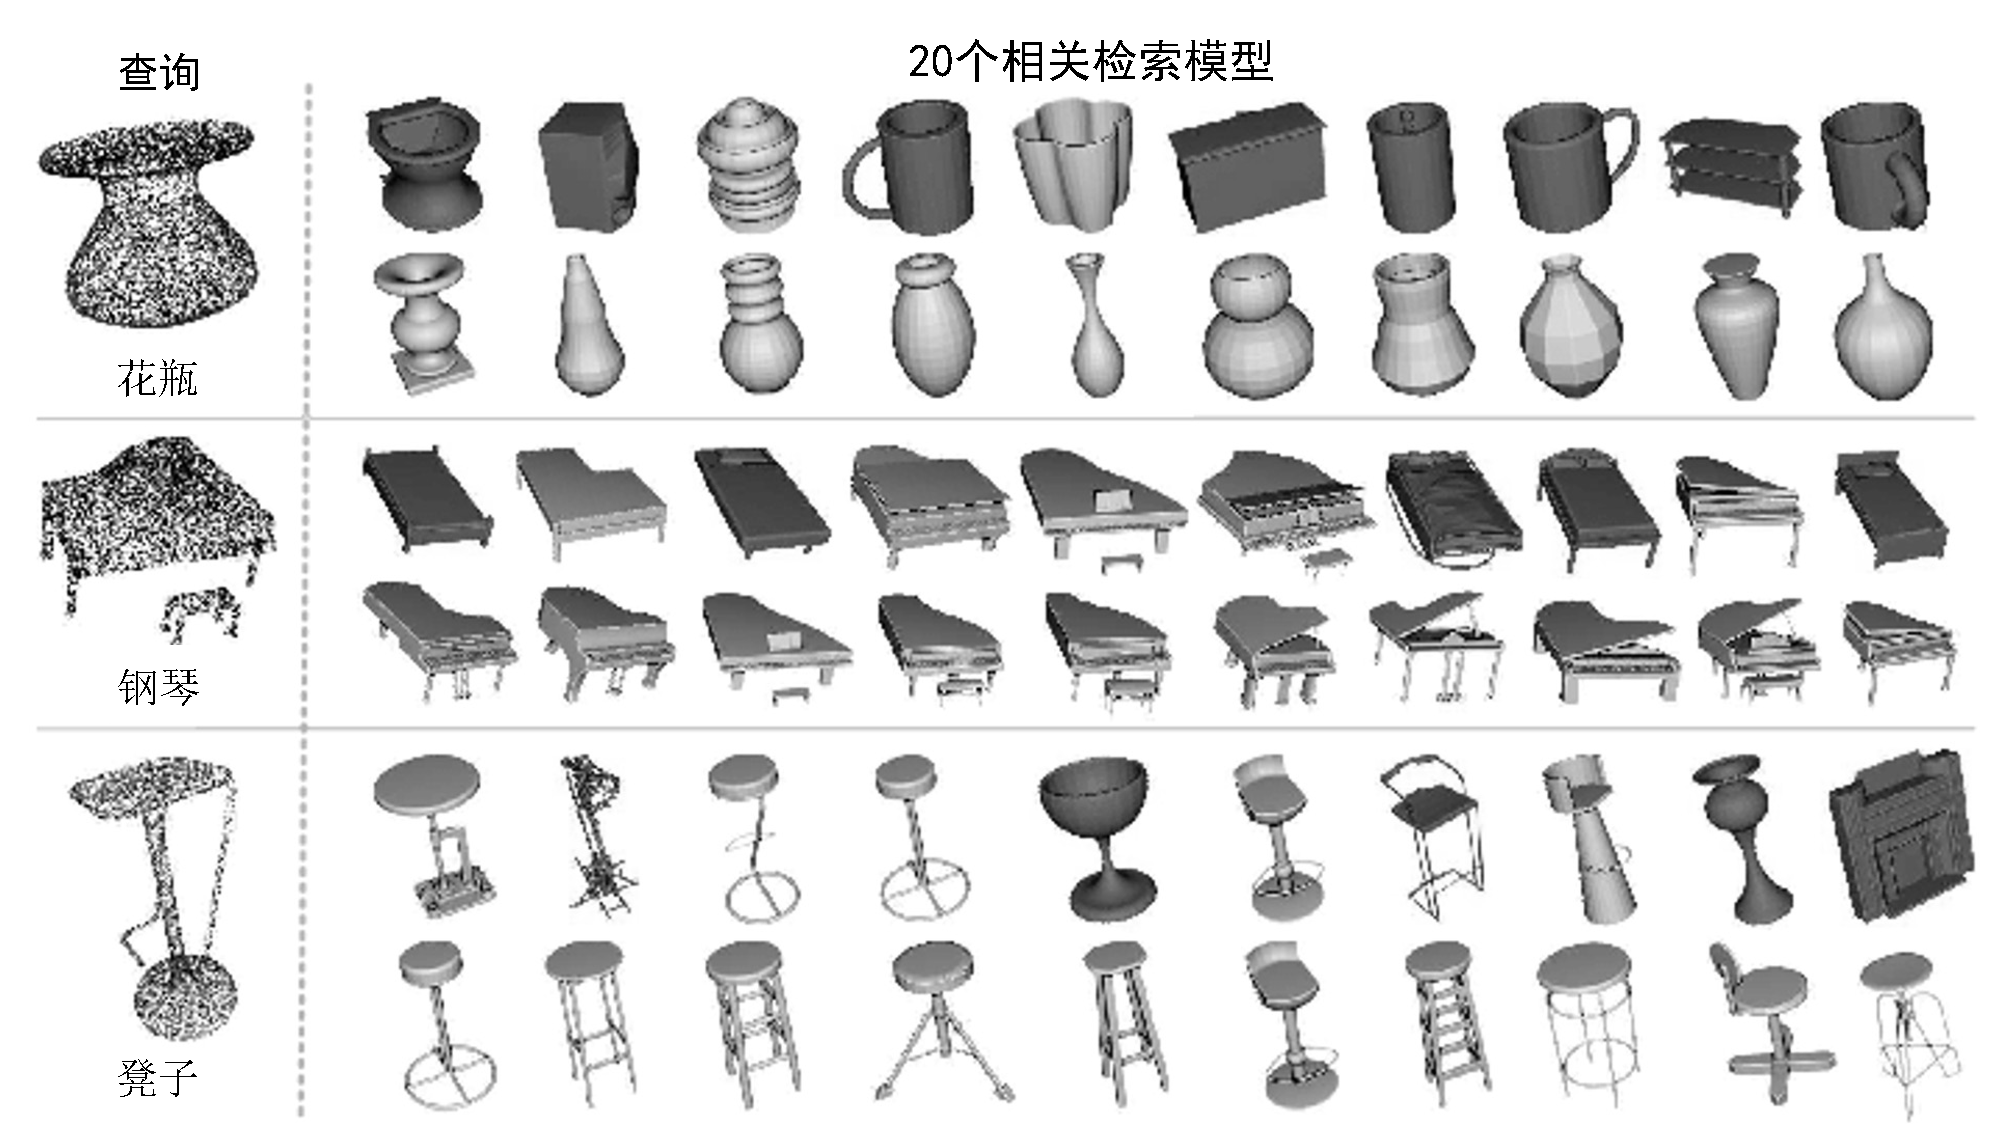
\includegraphics[width=\textwidth]{images/ModelNet.pdf}
    \caption{ModelNet40 数据集部分可视化结果}
    \label{fig:modelnet}
    \vspace{-0.5cm}
\end{figure}

\begin{figure}
    \centering
    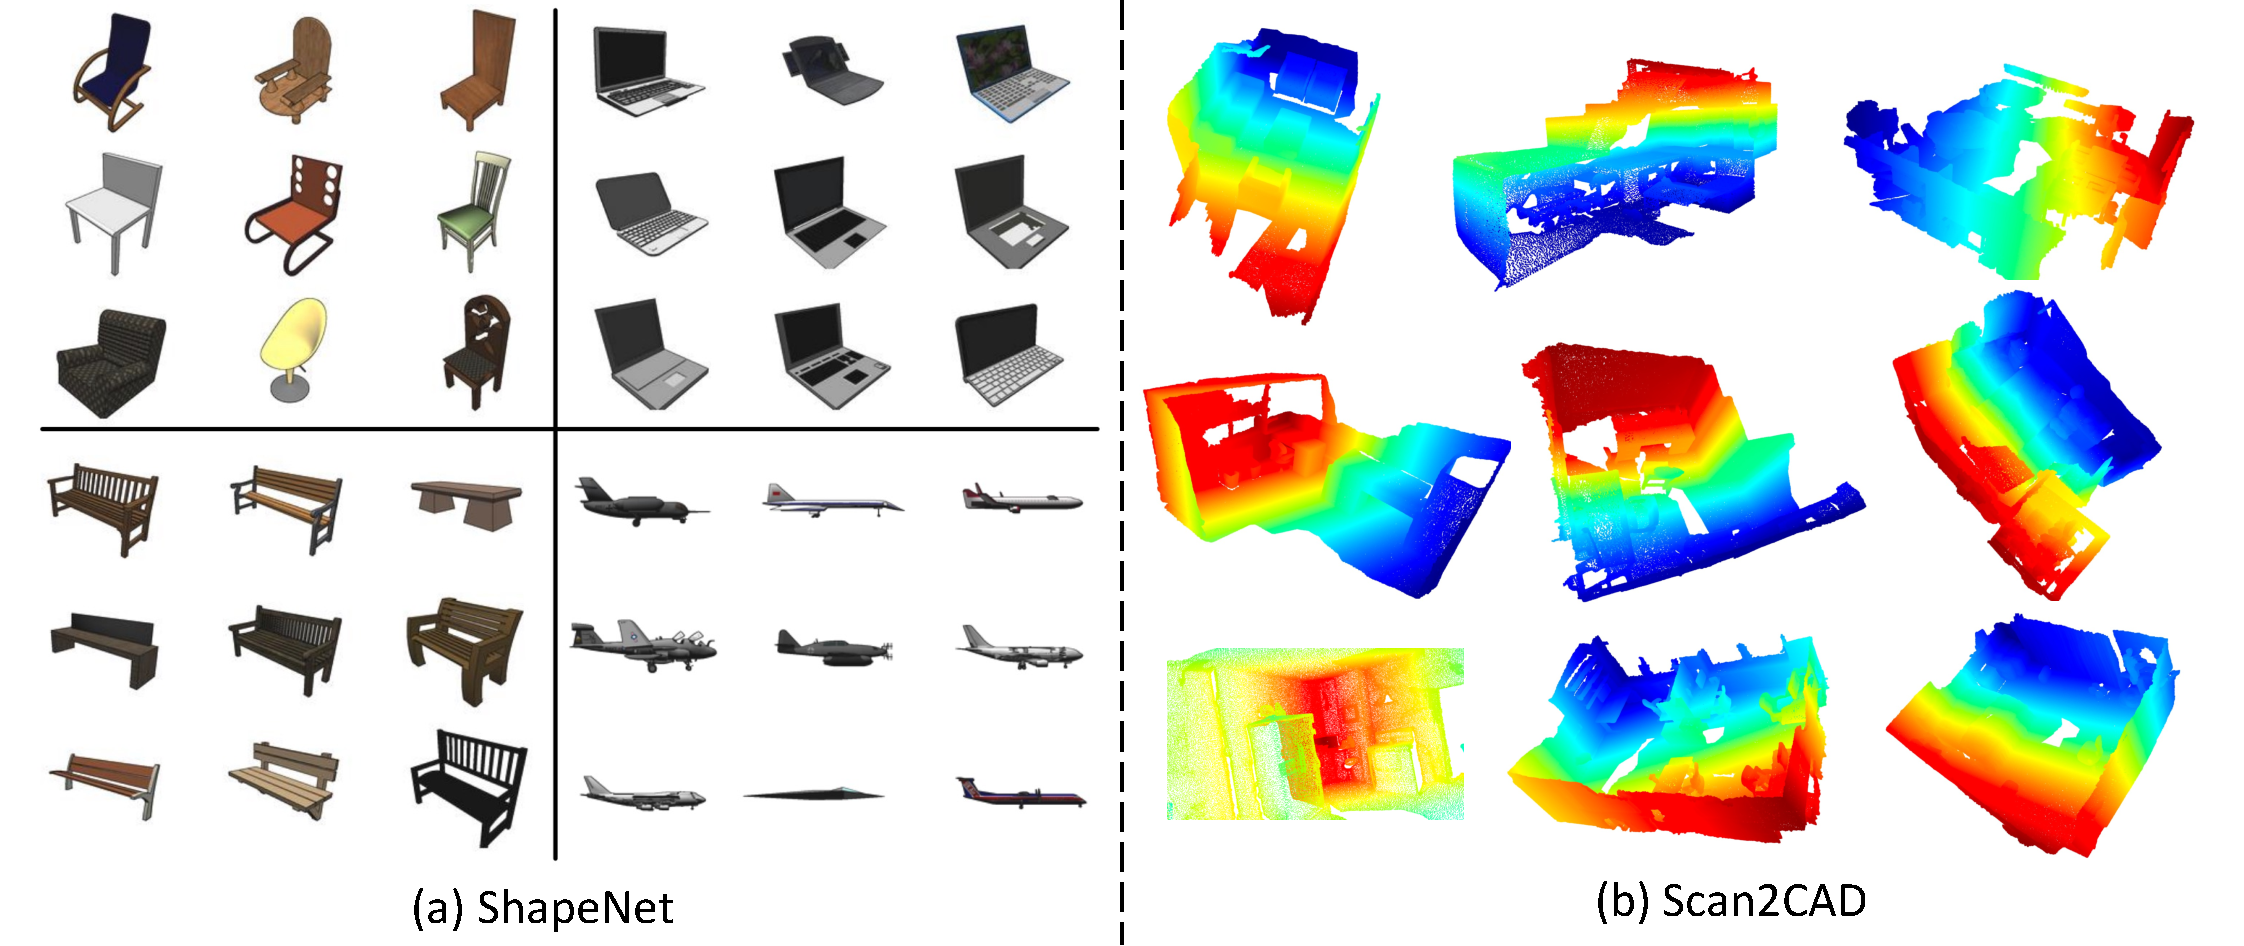
\includegraphics[width=\textwidth]{images/Shapenet-Scan2CAD.pdf}
    \caption{ShapeNet 数据集和Scan2CAD 数据集部分可视化结果}
    \label{fig:ShapeNet&Scan2CAD}
    \vspace{-0.5cm}
\end{figure}
\subsection{ShapeNet}
ShapeNet 数据集是一个大规模的三维模型数据库,其目的是为计算机视觉和图形学领域的研究者提供一个丰富且多样化的数据源。该数据集涵盖了许多不同的物体类别,包括家具、交通工具、家电等。ShapeNet 数据集中的模型具有详细的几何形状和丰富的语义标注,这使得它在多种三维任务中都具有很高的实用价值。

ShapeNet 数据集包含了 55 个类别,共有 51,190 个三维模型。这些模型主要来源于网上的 CAD 模型库,经过清洗和处理后整合成一个统一的数据集。数据集中的每个模型都以网格(mesh)格式存储,并附有与物体相关的语义信息,如类别标签、实例标签等。此外,ShapeNet 数据集还包含了一些额外的元数据,如模型的尺寸、位置和方向等。部分可视化结果如图\ref{fig:ShapeNet&Scan2CAD} (a) 所示。

\subsection{Scan2CAD}
Scan2CAD 数据集是一个用于场景理解和CAD模型对齐的大规模数据集。该数据集的目标是将真实场景的三维扫描与合成的CAD模型相关联。Scan2CAD 数据集包含了从Matterport3D\cite{chang2017matterport3d} 和 ScanNet\cite{dai2017scannet} 等公共数据集中的扫描数据,与来自ShapeNet等数据集的CAD模型。这些扫描和CAD模型之间的对应关系是通过专家注释来确定的。

Scan2CAD 数据集中的扫描数据包含了多种室内场景,如住宅、办公室和公共场所等。这些场景包括了各种物体,如家具、装饰品和建筑元素。与此同时,CAD模型包含了各种详细的几何和拓扑结构。部分可视化结果如图\ref{fig:ShapeNet&Scan2CAD} (b) 所示。

\subsection{多实例点云配准仿真数据集}
数据集:我们在合成数据集和真实数据集上进行实验。我们的合成数据集是从ModelNet40构建的,它包括来自40个类别的12311个网格化CAD模型。为了构建我们的合成数据集,对于每个模型,我们从中均匀地下采样1024个点以形成源点云,然后将其旋转和平移5-10次以生成多个实例。这些实例与噪声点混合,形成如图3所示的目标点云。沿每个轴的旋转在[0,180°]内均匀采样,平移在[0,5]内。我们为合成数据集生成的输入对应关系是通过将真实对应关系与异常值混合而生成的。我们将每个实例的内点比率控制在约2\%。我们使用12311个模型生成了12311个这样的合成源-目标点云对。我们使用9843对进行训练,2468对进行测试。我们在训练集中随机留出10\%的对作为验证集。

\subsection{多实例点云配准真实数据集}
我们的真实数据集是 Scan2CAD ,它利用 ShapeNet 和 ScanNet 构建而成。此数据集使用 ShapeNet 中的 CAD 模型替换真实扫描场景中的点云,并提供精确的注释,包括模型类别、旋转和平移等。数据集提供了 1506 个带注释的场景,每个场景至少包含一个实例类别。因此,我们充分利用这些注释,并将包含多种实例的场景分割成多个源-目标点云对,用于多实例注册。通过这种方式,我们得到了 2184 对点云,其中大多数点云在目标点云中包含 2-5 个相同类别的实例。我们按照 7:1:2 的比例将样本划分为训练集、验证集和测试集。我们使用微调的 FCGF\cite{FCGF2019} 生成局部特征并通过特征匹配生成假设的对应关系。
\begin{table}[h]
    \centering
    \vspace{-1.0cm}
    \begin{minipage}{0.45\textwidth}
        \centering
        \caption{FCGF 网络参数设置和预训练}
        \label{tab:fcgf}
        \begin{tabular}{cc}
        \toprule
        \multicolumn{2}{c}{FCGF 网络参数设置和预训练} \\ 
        \midrule
        模型                 & RESUNETBN2C      \\ 
        下采样体素大小          & 2.5cm (0.025)    \\ 
        特征维度                & 32               \\ 
        预训练数据集             & 3DMatch          \\ 
        特征归一化              & 是               \\ 
        \bottomrule
        \end{tabular}
    \end{minipage}
    \hfill
    \begin{minipage}{0.45\textwidth}
        \centering
        \caption{FCGF 网络微调参数设置}
        \label{tab:fcgf_finetune}
        \begin{tabular}{cc}
        \toprule
        \multicolumn{2}{c}{FCGF 网络微调参数设置} \\ 
        \midrule
        批量大小               & 4                 \\ 
        学习率                 & $10^{-3}$         \\ 
        迭代次数                & 20                \\ 
        优化器                 & SGD               \\ 
        \bottomrule
        \end{tabular}
    \end{minipage}
    \vspace{-1.0cm}
\end{table}

这里,我们主要关注如何通过特征匹配生成假设的对应关系。我们使用 FCGF 作为特征提取器,参数设置如表 \ref{tab:fcgf} 所示。FCGF 网络在 3DMatch 数据集上预训练,然后使用表 \ref{tab:fcgf_finetune} 中的参数设置进行微调。微调过的 FCGF 提取 L2归一化的局部特征 $F_{local}^X = \{f_{local}^{x_i} \in \mathbb{R}^{32} | i = 1, \dots, |X|\}$,用于源点云 $X$ 和 $F_{local}^Y = \{f_{local}^{y_i} \in \mathbb{R}^{32} | i = 1, \dots, |Y|\}$,用于目标点云 $Y$,其中 $|X|$ 和 $|Y|$ 分别表示源点云和目标点云中的点数。给定目标点云 $Y$ 中的每个点 $y_j$,我们找到满足 $i = \arg\max_i \langle f_{local}^{y_j}, f_{local}^{x_i} \rangle$ 的源点云 $X$ 中的点 $x_i$ 以构建对应关系 $(x_i, y_j)$,其中 $\langle f_{local}^{y_j}, f_{local}^{x_i} \rangle$ 是两点特征之间的余弦相似度。这样,我们获得 $|Y|$ 个对应关系,我们将余弦相似度 $\langle f_{local}^{x_i}, f_{local}^{y_j} \rangle$ 定义为对应关系 $(x_i, y_j)$ 的显著性得分。我们选择显著性得分最大的 $K$ 个对应关系,然后将这些 $K$ 个对应关系随机下采样为 $N$ 个对应关系作为输入的假设对应关系。这里,我们将 $K$ 设置为 10000,以使输入对应关系尽可能覆盖更多实例。
\section{点云配准评价指标}
对于配准任务,评估指标可以主要分为两类,一类是用于特征提取与匹配的评价指标,另一类是用于配准结果运动参数评价的指标。
\subsection{基于特征提取与匹配的评价指标}
\subsubsection{特征匹配召回率 (Feature Matching Recall)}
特征匹配召回率衡量了匹配算法在正确提取匹配点对数量和所有点对数量之间的比率,反映了匹配算法的查全率。从数学角度来看,特征匹配召回率可以表示为:
\begin{equation}
R_{fa} = \frac{1}{n} \sum_{s=1}^{n} \mathbbm{1} \left( \frac{1}{|\boldsymbol{\omega}|} \sum_{(\boldsymbol{i},\boldsymbol{j})\in\boldsymbol{\omega}} (\lVert \boldsymbol{T}\boldsymbol{p}_i - \boldsymbol{q}_j \rVert < \tau_1) > \tau_2 \right)
\end{equation}
其中 $n$ 是所有点对的数量,$\boldsymbol{\omega}$ 是匹配点对 $(\boldsymbol{p}, \boldsymbol{q})$ 之间的对应关系集合,$\boldsymbol{p} = (x_p, y_p, z_p)$,$\boldsymbol{q} = (x_q, y_q, z_q)$,$\boldsymbol{T} \in SE(3)$ 是地面真实姿态变换矩阵。此外,$\tau_1$ 是内部距离阈值,$\tau_2$ 是内部召回率阈值。
\subsubsection{点云配准召回率 (Point Cloud Registration Recall)}
配准召回率衡量了在具有地面真实姿态变换且存在重叠部分的两组点云中,有多少重叠部分的点云组可以通过匹配算法被正确恢复。具体而言,配准召回率使用如下误差矩阵来定义真阳性:
\begin{equation}
    E = \sqrt{\frac{1}{|\boldsymbol{\omega}^*|} \sum_{(\boldsymbol{p}^*,\boldsymbol{q}^*)\in\boldsymbol{\omega}^*} \lVert \boldsymbol{\hat{T}}_{i,j}\boldsymbol{p}^* - \boldsymbol{q}^* \rVert^2} < \tau_3
\end{equation}
    
其中,$\boldsymbol{\omega}^*$ 是重叠部分一组匹配点对 $(\boldsymbol{p}^*, \boldsymbol{q}^*)$ 之间的对应关系集合,$\boldsymbol{p}^* = (x^*_p, y^*_p, z^*_p)$,$\boldsymbol{q}^* = (x^*_q, y^*_q, z^*_q)$。对于重叠部分,$\tau_3$ 是用于判断匹配点对是否正确的阈值。

\subsection{基于刚体运动的评价指标}
\subsubsection{投影的均方根误差}
投影的均方根误差 (RMSE Projection) 是在应用变换之后,计算点到点投影误差的平均值。计算公式为:
\begin{equation}
    \text{RMSE} (\boldsymbol{p}) = \frac{1}{n}\sum_{i=1}^{n} \sqrt{(\boldsymbol{p}_i^{'} - \boldsymbol{p}_i)^2},
\end{equation}
其中 $n$ 是点云中的点数,$\boldsymbol{p}_i^{'}$ 是应用变换后的点,$\boldsymbol{p}_i$ 是原始点。

\subsubsection{变换的均方根误差}
变换的均方根误差 (RMSE Tranformation) 代表估计的变换 $\boldsymbol{\hat{T}}_{s}$ 和真实变换 $\boldsymbol{T}^*_{s}$ 之间的均方根误差。计算公式为:
\begin{equation}
    \text{RMSE} (\boldsymbol{T}) = \sqrt{\frac{1}{n}\sum_{i=1}^{n}(\boldsymbol{\hat{T}}_{s} - \boldsymbol{T}^*_{s})^2},
\end{equation}

\subsubsection{相对旋转误差}
我们定义相对旋转误差 (Relative Rotation Error) 为真实变换 $\boldsymbol{T}^*_{s}$ 和估计变换 $\boldsymbol{\hat{T}}_{s}$ 之间的旋转误差。计算公式为:
\begin{equation}
    \text{RRE}_s = \arccos \left(\frac{\operatorname{tr}(\boldsymbol{\hat{R}}_{s} \boldsymbol{R}^*_s) - 1}{2}\right),
\end{equation}
其中 $\operatorname{tr}$ 表示矩阵的迹(对角线元素之和),$\boldsymbol{\hat{R}}_{s}$ 和 $\boldsymbol{R}^*_s$ 分别表示估计变换和真实变换的旋转矩阵。

\subsubsection{相对平移误差}
我们定义相对平移误差 (Relative Transition Error) 为真实变换 $\boldsymbol{T}^*_s$ 和估计变换 $\boldsymbol{\hat{T}}_{s}$ 之间的平移误差。计算公式为:
\begin{equation}
    \text{RTE}_s = \lVert \boldsymbol{t}^*_s - \boldsymbol{\hat{t}}_{s} \rVert,
\end{equation}
其中 $\boldsymbol{t}^*_s$ 和 $\boldsymbol{\hat{t}}_{s}$ 分别表示真实变换和估计变换的平移向量。

\subsection{多实例点云配准评价指标}
\label{sec:multiinstance_eval}
用于评估多实例点云配准性能的三个指标分别是平均命中召回率、平均命中精度和平均命中 F1 分数。

\subsubsection{平均命中召回率 (Mean Hit Recall)}
平均命中召回率衡量了正确恢复的点云对数占所有点云对数的比例。平均命中召回率 (Mean Hit Recall) 在两个已配准的点云之间的定义如下:
\begin{equation}
    \text{MHR} = \frac{1}{\boldsymbol{K}} \sum_{s=1}^{S} \boldsymbol{I}_s
\end{equation}
其中 $\boldsymbol{I}_s = {0, 1}$ 表示一个真实估计对是否为“命中”。具体而言,
\begin{equation}
    \boldsymbol{I}_s = \boldsymbol{I}(\text{RRE}_s < \tau_r) \times \boldsymbol{I}(\text{RTE}_s < \tau_t)
\end{equation}
其中 $\boldsymbol{I}(\cdot) = {0, 1}$ 表示一个指示函数。$\text{RRE}_s$ 和 $\text{RTE}_s$ 是第 $s$ 个真实估计对的相对旋转误差和相对平移误差。两个阈值 $\boldsymbol{\tau_r}$ 和 $\boldsymbol{\tau_t}$ 分别设置为 $20^\circ$ 和 $0.5m$。通过对所有点云对的 \text{MHR} 求平均值,得到最终的平均命中召回率。

\subsubsection{平均命中精确度 (\text{Mean Hit Precision})}
两个已配准的点云之间的平均命中精确度定义如下:

\begin{equation}
\text{MHP} = \frac{1}{\boldsymbol{M}} \sum_{s=1}^{S} \boldsymbol{I}_s
\end{equation}
通过对所有点云对的 \text{MHP} 求平均值,得到最终的平均命中精确度。

\subsubsection{平均命中 F1 (\text{Mean Hit F1})}
两个已配准的点云之间的平均命中 F1 定义如下:
\begin{equation}
\text{MHF1} = \frac{2 \times \text{MHP} \times \text{MHR}}{\text{MHP} + \text{MHR}}
\end{equation}
通过对所有点云对的 \text{MHF1} 求平均值,得到最终的平均命中 F1。


\section{点云处理与配准相关深度学习技术}

\subsection{深度学习概述}
在过去的十年中,深度学习在计算机视觉、自然语言处理等各个领域取得了重要进展 \cite{lecun2015deep}。随着激光雷达、RGB-D 相机和其他三维扫描设备获取的 3D 数据日益增多,深度学习技术逐渐应用于点云处理任务,包括点云配准 \cite{wang2019dynamic, choy2020deep}。点云配准是 3D 计算机视觉中的一个基本问题,目的是找到将两个点云精确对齐的最优变换。

近年来,针对点云配准的深度学习方法已经在自动学习区分性特征和从大规模数据集中学习鲁棒匹配策略方面展示出优于传统方法的性能 \cite{huang2022multiway, lu2019deepvcp}。这些方法利用各种类型的网络架构,例如 PointNet \cite{qi2017pointnet}、PointNet++ \cite{qi2017pointnet++} 和 DGCNN \cite{wang2019dynamic},有效地处理点云数据的非结构化和无序特性。

训练深度神经网络涉及使用反向传播算法,该算法通过应用链式法则计算损失函数相对于每个权重的梯度。使用基于梯度的优化方法(如随机梯度下降(SGD)、Adam\cite{kingma2014adam} 或 MoCo\cite{he2020momentum})更新权重。为了防止过拟合,采用了如 dropout 等正则化技术,即在训练过程中随机将一层中的一部分神经元设置为零。这种策略迫使网络学习更鲁棒的特征,提高了对未见数据的泛化能力。

\begin{equation}
    L(\boldsymbol{W}) = \frac{1}{N} \sum_{i=1}^{N} L_i(\boldsymbol{W}) + \lambda \sum_{l=1}^{L} \lVert \boldsymbol{W}^{(l)} \rVert^2
\end{equation}

在上述方程中,$L(\boldsymbol{W})$ 表示总损失,$L_i(\boldsymbol{W})$ 表示第 $i^{th}$ 个样本的损失,$\boldsymbol{W}^{(l)}$ 表示第 $l$ 层的权重,$L$ 是总层数,$\lambda$ 是正则化参数,$\lVert \cdot \rVert^2$ 表示平方 Frobenius 范数。

为了方便设计、训练和部署深度学习模型,开发了几种深度学习框架,包括TensorFlow\cite{abadi2016tensorflow}、PyTorch\cite{paszke2019pytorch}、PaddlePaddle\cite{ma2019paddlepaddle} 和 MXNet\cite{chen2015mxnet}。这些框架提供了神经网络层、优化算法和其他实用工具的高效实现,使设计、训练和部署深度学习模型变得更加容易。此外,它们还支持使用 GPU (torch.cuda)或专用加速器(如 TPU)进行硬件加速,以加快训练过程。
\subsection{多层感知机}
多层感知器(Multilayer Perceptron, MLP)是一种广泛应用于各种机器学习任务的前馈神经网络\cite{lecun2015deep}。MLP 的基本结构包括输入层、一个或多个隐藏层和输出层。每一层由若干个神经元组成,相邻层的神经元之间通过权重连接。通常,MLP 采用全连接结构,即每个神经元都与上一层和下一层的所有神经元连接。

在训练 MLP 时,需要先进行前向传播计算,即从输入层到输出层计算预测值。接下来,通过反向传播算法计算损失函数对权重的梯度。最后,使用梯度下降或其变体更新权重。

考虑一个简单的两层 MLP,其输入层有 $n$ 个神经元,输出层有 $m$ 个神经元。对于输入向量 $\boldsymbol{x} \in \mathbb{R}^{n}$ 和权重矩阵 $\boldsymbol{W} \in \mathbb{R}^{m \times n}$,MLP 的输出为:

\begin{equation}
\boldsymbol{y} = f(\boldsymbol{W}\boldsymbol{x} + \boldsymbol{b}),
\end{equation}

其中 $\boldsymbol{b} \in \mathbb{R}^{m}$ 是偏置向量,$f$ 是激活函数。在实际应用中,激活函数通常为非线性函数,如 Sigmoid、ReLU 或 Tanh。这些非线性激活函数使得 MLP 能够捕捉复杂的非线性关系。

现在我们考虑一个具有 $L$ 个隐藏层的 MLP,设第 $l$ 层的权重矩阵为 $\boldsymbol{W}^{(l)} \in \mathbb{R}^{n_l \times n_{l-1}}$,偏置向量为 $\boldsymbol{b}^{(l)} \in \mathbb{R}^{n_l}$,激活函数为 $f^{(l)}$。前向传播过程可表示为:

\begin{equation}
\boldsymbol{a}^{(l)} = f^{(l)}(\boldsymbol{W}^{(l)}\boldsymbol{a}^{(l-1)} + \boldsymbol{b}^{(l)}),
\end{equation}

其中 $\boldsymbol{a}^{(0)} = \boldsymbol{x}$,$\boldsymbol{a}^{(L)} = \boldsymbol{y}$。对于损失函数 $L(\boldsymbol{y}, \boldsymbol{t})$,其中 $\boldsymbol{t}$ 是目标输出,我们使用梯度下降方法优化权重和偏置:

\begin{equation}
\boldsymbol{W}^{(l)} \leftarrow \boldsymbol{W}^{(l)} - \alpha \frac{\partial L}{\partial \boldsymbol{W}^{(l)}}, \\
\end{equation}
\begin{equation}
\boldsymbol{b}^{(l)} \leftarrow \boldsymbol{b}^{(l)} - \alpha \frac{\partial L}{\partial \boldsymbol{b}^{(l)}},
\end{equation}

其中 $\alpha$ 是学习率。

为了计算梯度,我们使用反向传播算法。首先,计算输出层关于损失函数的梯度:

\begin{equation}
\boldsymbol{\delta}^{(L)} = \frac{\partial L}{\partial \boldsymbol{a}^{(L)}} \odot f'^{(L)}(\boldsymbol{W}^{(L)}\boldsymbol{a}^{(L-1)} + \boldsymbol{b}^{(L)}),
\end{equation}

其中 $\odot$ 表示哈达玛积(元素对应相乘),$f'^{(L)}$ 是激活函数的导数。

然后,我们从输出层向输入层反向计算梯度:

\begin{equation}
\boldsymbol{\delta}^{(l)} = \left( \boldsymbol{W}^{(l+1)} \right)^T \boldsymbol{\delta}^{(l+1)} \odot f'^{(l)}(\boldsymbol{W}^{(l)}\boldsymbol{a}^{(l-1)} + \boldsymbol{b}^{(l)}).
\end{equation}

最后,我们计算损失函数关于权重和偏置的梯度:

\begin{equation}
\frac{\partial L}{\partial \boldsymbol{W}^{(l)}} = \boldsymbol{\delta}^{(l)} \left( \boldsymbol{a}^{(l-1)} \right)^T, \\
\end{equation}
\begin{equation}
\frac{\partial L}{\partial \boldsymbol{b}^{(l)}} = \boldsymbol{\delta}^{(l)}.
\end{equation}

在实际应用中,为了提高训练速度和泛化能力,我们通常采用 mini-batch 随机梯度下降或其变体(如 Adam、RMSprop 等)进行训练。此外,我们还可以使用正则化技术(如 L1、L2正则化、Dropout 等)防止过拟合。在深度学习框架(如 TensorFlow、PyTorch、PaddlePaddle 和 MXNet 等)的支持下,我们可以方便地实现和训练 MLP 模型\cite{lecun2015deep}。

MLP 是深度学习领域的一个基本概念,尽管现在有许多更复杂的神经网络结构(如卷积神经网络、循环神经网络和 Transformer 等)已经在各种任务上表现出更好的性能,但 MLP 仍然是一个重要的基础知识。通过学习 MLP 的基本原理,我们可以更好地理解神经网络的工作原理,从而有助于设计更复杂的模型和解决更高级的问题。

在实际应用中,MLP 可以处理各种类型的数据,如图像、文本、语音和其他结构化或非结构化数据。由于 MLP 可以近似任意连续函数,因此具有很强的表达能力。然而,MLP 也存在一些局限性。首先,MLP 的参数数量随着层数和每层神经元数量的增加而快速增长,这可能导致过拟合和计算效率低下的问题。其次,MLP 对输入数据的缩放和平移具有较强的敏感性,因此需要对输入数据进行预处理,如归一化。此外,MLP 并不能直接处理变长输入数据和序列数据,需要采用其他神经网络结构,如循环神经网络(RNN)。

尽管如此,MLP 作为一种基础的神经网络结构,在许多任务中仍具有竞争力。例如,在监督学习任务中,MLP 可以用于分类和回归问题;在无监督学习任务中,MLP 可以用于降维和聚类。通过合适的设计和训练策略,MLP 能够在各种应用场景中实现良好的性能。

总之,多层感知器(MLP)是深度学习领域的一个基本概念,作为前馈神经网络的一种,它具有广泛的应用价值。MLP 主要包括输入层、隐藏层和输出层,通过前向传播、反向传播算法进行训练。
\subsection{卷积神经网络}
卷积神经网络(CNN)是一类在各种任务中取得显著成功的深度学习模型,尤其在图像识别、目标检测和自然语言处理等领域。CNN 旨在学习空间特征层次结构,使其特别适用于处理网格状数据(如图像),其中局部依赖关系至关重要\cite{chua1993cnn}。

CNN 的基本构建模块是卷积层。在这个层中,小滤波器(也称为内核)应用于输入,计算滤波器和输入之间的局部点积。这个操作生成一个特征映射,对输入和滤波器之间的空间关系进行编码\cite{he2016deep}。滤波器权重在训练过程中学习,使网络能够自动学习任务特定特征。

从数学上讲,CNN 中的卷积运算可以描述为以下形式:

\begin{equation}
  y_{i,j} = \sum_{m} \sum_{n} x_{i-m, j-n} \cdot w_{m,n},
\end{equation}

其中 $x$ 是输入,$w$ 是滤波器,$y$ 是输出特征映射,$i$、$j$、$m$ 和 $n$ 是输入和滤波器的空间维度对应的索引。

CNN 的一个关键方面是在整个输入中使用共享权重。这种参数共享显著减少了可训练参数的数量,使模型比全连接网络更具计算效率且不容易过拟合。此外,它使网络能够学习平移不变特征,因为相同的滤波器应用于输入的不同空间位置。

CNN 中的另一个重要组件是池化层,用于减少特征映射的空间尺寸。池化层通常在一个或多个卷积层之后应用,以实现局部平移不变性并减少网络的计算复杂性。有不同类型的池化操作,如最大池化、平均池化和全局池化。最大池化是最常用的池化方法,可以定义为:

\begin{equation}
  z_{i,j} = \max_{m,n \in P} x_{i+m, j+n},
\end{equation}

其中 $x$ 是输入特征映射,$z$ 是池化后的输出,$P$ 是池化窗口,$i$、$j$、$m$ 和 $n$ 是输入和池化窗口的空间维度对应的索引。

除了卷积和池化层之外,CNN 通常包括一个或多个全连接层,对学习到的特征进行高级推理。最后一个全连接层的输出通常通过 softmax 激活函数传递,以生成任务特定类别的概率。整个网络使用反向传播和基于梯度的优化算法(如随机梯度下降或 Adam)进行训练。

CNN 已成功应用于广泛的任务,包括图像分类、目标检测、语义分割和自然语言处理。CNN 的成功可以归因于其学习输入数据的分层表示、共享权重和平移不变特征的能力。此外,通过修改其架构和损失函数,CNN 可以轻松地适应不同的任务\cite{albawi2017understanding}。

\subsection{注意力机制}
注意力机制已经成为深度学习模型的重要组成部分,特别是在计算机视觉和点云处理任务中。注意力机制的核心概念是让模型在处理输入数据时,根据上下文信息有选择地关注不同部分,从而提高性能和可解释性。

在计算机视觉领域,注意力机制可以帮助模型更有效地识别和关注图像中的重要区域,以实现更准确的对象识别、语义分割和目标检测。在点云处理任务中,注意力机制可以帮助模型学习点云中的局部和全局结构特征,从而在点云配准、点云分割和分类任务中实现更高的性能。

数学上,注意力机制可以通过以下方式进行描述:

\begin{equation}
\text{Attention}(\boldsymbol{Q}, \boldsymbol{K}, \boldsymbol{V}) = \text{softmax}(\frac{\boldsymbol{Q}\boldsymbol{K}^\top}{\sqrt{d_k}})\boldsymbol{V},
\end{equation}

其中 $\boldsymbol{Q}$、$\boldsymbol{K}$ 和 $\boldsymbol{V}$ 分别表示查询(Query)、键(Key)和值(Value)矩阵,$d_k$ 是键和查询向量的维度。这个计算过程可以解释为:查询向量与键向量的点积表示它们之间的相似性,通过应用 softmax 函数将这些相似性归一化为概率分布,然后使用这些概率分布加权值向量,得到最终的输出。

在计算机视觉和点云处理任务中,注意力机制通常与卷积神经网络(CNN)或图神经网络(GNN)结合使用,以捕获局部和全局上下文信息。这些组合模型在大量基准数据集上表现出卓越的性能,证明了注意力机制在这些领域的有效性。


\section{基于深度学习的点云配准方法}
本节主要阐述主要的基于深度学习的点云配准方法作为基准线,主要阐述PointNet\cite{qi2017pointnet, qi2017pointnet++}系列框架、Predator\cite{huang2021predator}描述子和TEASER\cite{yang2020teaser}配准方法。

\subsection{PointNet \& PointNet++}
\begin{figure}
    \centering
    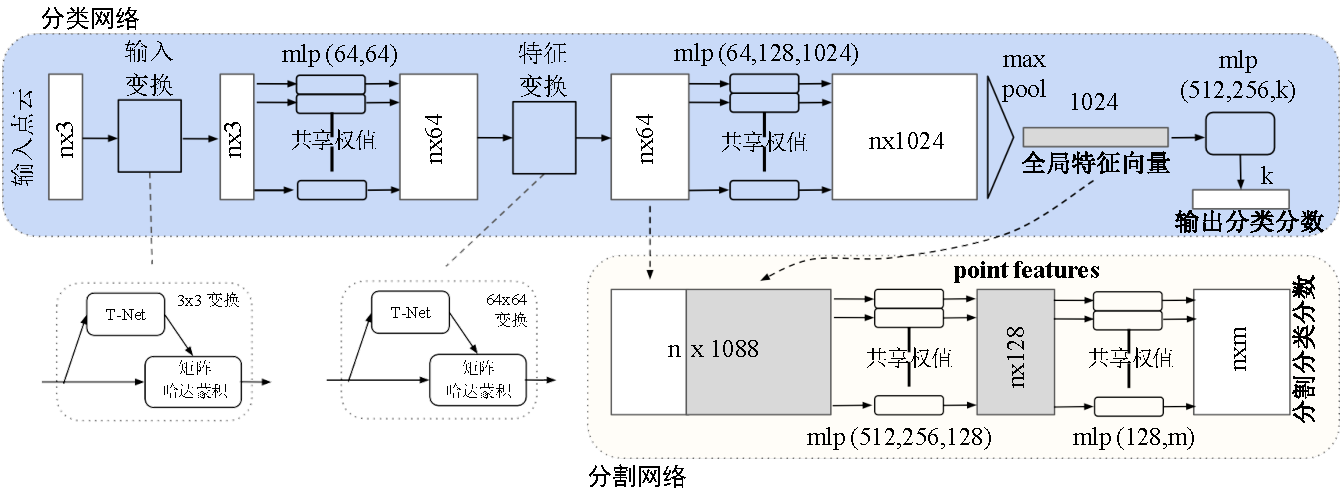
\includegraphics[width=\linewidth]{images/pointnet.pdf}
    \caption{PointNet\cite{qi2017pointnet}网络结构图}
    \label{fig:pointnet}
    \vspace{-5mm}
\end{figure}

\subsubsection{PointNet}
点云处理任务中,我们首先可以朴素地想到直接用多层感知机\cite{lecun2015deep}对作为点云的输入,但是这样的方法对于$N$个点云来说,需要$N \times 3$大小的输入维度,点云数量多时,对于多层感知机过于庞大。所以PointNet提出,对于输入点云,采用共享权值的MLP进行特征提取
\begin{equation}
    \boldsymbol{f_p}_i = f(\theta; \boldsymbol{p}_i)
\end{equation}
然后对特征进行特征变换,对于变换后的特征再次进行升维操作,最终通过$n$个点云数据,得到$n \times 1024$的特征图。将特征图进行最大吃池化操作,得到全局特征向量。

对于分类任务,每一个点云对应一个类别,所以全局特征可以直接用来判断类别信息,通过一个MLP输出最终的分类分数,达到分类的效果。对于点云分割任务,全局特征不足以描述分割的模式,需要加入局部特征。所以将全局特征向量和$\boldsymbol{f_p}_i$进行拼接操作,得到局部+全局特征,通过MLP输出分割的分类分数。

\subsubsection{PointNet++}
PointNet++\cite{qi2017pointnet++}则在PointNet上做了改进。前文提到的PointNet在点云处理中有一个重大缺陷,即点云是具有丰富的表面几何特征的数据格式,也就是说,每一个点都和周围的点产生了交互,但是PointNet仅仅提取出了点的特征和全局特征,缺失了提取局部特征这一过程。这在训练神经网络的时候,往往会导致模型的泛化能力有限\cite{qi2017pointnet++}。所以PointNet++对此作出了调整,在PointNet的基础上提去了不同尺度的局部特征,图示如图\ref{fig:pointnet++}。

\begin{figure}
    \centering
    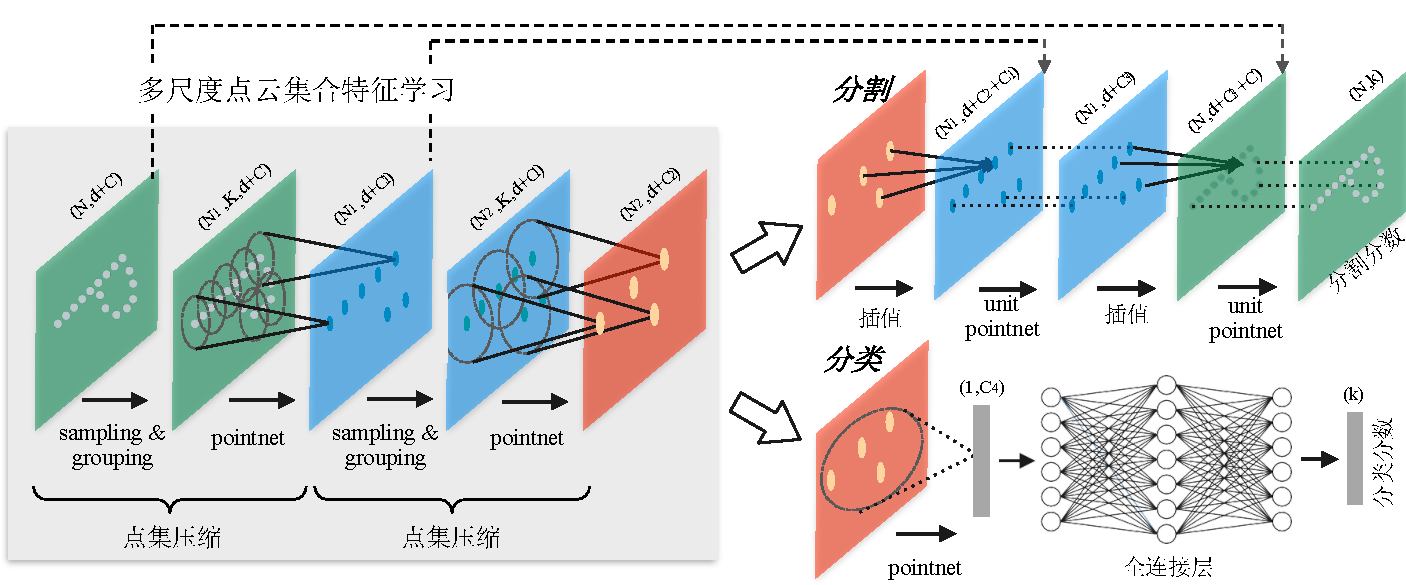
\includegraphics[width=\linewidth]{images/pointnet++.pdf}
    \caption{PointNet++\cite{qi2017pointnet++}网络结构图}
    \label{fig:pointnet++}
    \vspace{-5mm}
\end{figure}

这个方法是受到CNN的启发,在3D点集中找到具有相似结构的子区域,和对应的区域特征embedding,提出了Sampling和Grouping来整合局部邻域的点云,提取局部特征,代码如\ref{lst:pythonfile}。其中,\texttt{farthest point sample}为本段的核心算法,即最远端采样算法来实现从$N$个点中抽取采样$N'$个点。

最远端采样算法 (FPS)的流程如下:
1. 用蒙特卡洛方法筛取初始点,即第0次采样点; \\
2. 计算未采样点与已采样点之间的欧几里得或者推土机距离,将距离最大的点加入已采样点集; \\
3. 更新距离函数,重复1-3,直到获得了目标数量的采样点; \\

\begin{lstlisting}[language=Python, caption={Sampling}, label={lst:pythonfile}]
    def sample_and_group(npoint, radius, nsample, xyz, points, knn=False, use_xyz=True):
    '''
    Input:
        npoint: int32
        radius: float32
        nsample: int32
        xyz: (batch_size, ndataset, 3) TF tensor
        points: (batch_size, ndataset, channel) TF tensor, if None will just use xyz as points
        knn: bool, if True use kNN instead of radius search
        use_xyz: bool, if True concat XYZ with local point features, otherwise just use point features
    Output:
        new_xyz: (batch_size, npoint, 3) TF tensor
        new_points: (batch_size, npoint, nsample, 3+channel) TF tensor
        idx: (batch_size, npoint, nsample) TF tensor, indices of local points as in ndataset points
        grouped_xyz: (batch_size, npoint, nsample, 3) TF tensor, normalized point XYZs
            (subtracted by seed point XYZ) in local regions
    '''
    new_xyz = gather_point(xyz, farthest_point_sample(npoint, xyz)) # (batch_size, npoint, 3)
    if knn:
        _,idx = knn_point(nsample, xyz, new_xyz)
    else:
        idx, pts_cnt = query_ball_point(radius, nsample, xyz, new_xyz)
    grouped_xyz = group_point(xyz, idx) # (batch_size, npoint, nsample, 3)
    grouped_xyz -= tf.tile(tf.expand_dims(new_xyz, 2), [1,1,nsample,1]) # translation normalization
    if points is not None:
        grouped_points = group_point(points, idx) # (batch_size, npoint, nsample, channel)
        if use_xyz:
            new_points = tf.concat([grouped_xyz, grouped_points], axis=-1) # (batch_size, npoint, nample, 3+channel)
        else:
            new_points = grouped_points
    else:
        new_points = grouped_xyz
    return new_xyz, new_points, idx, grouped_xyz
\end{lstlisting}

上面介绍了如何从采样点到局部特征提取的过程,但是在实践中,提取到的不同尺度的特征如何融合对于下游任务的影响也同样很大。PointNet++提出了两种特征融合方式 Multi-Scale Grouping (MSG) 和 Multi-Resolution Grouping (MRG)。如图\ref{fig:pnpp_grouping}(a)、(b)所示。

\begin{figure}[H]
    \vspace{-5mm}
    \centering
    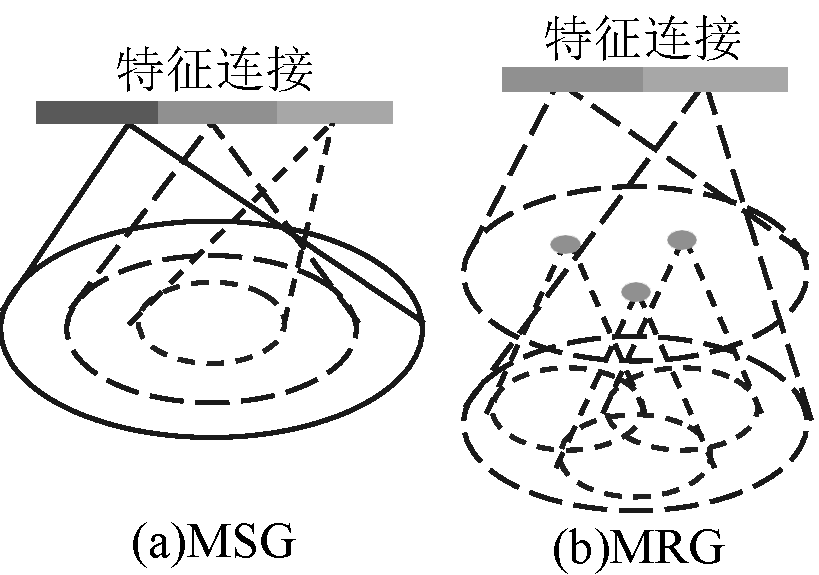
\includegraphics[width=0.45\linewidth]{images/pnpp_group.pdf}
    \caption{多尺度特征融合方法示意图}
    \label{fig:pnpp_grouping}
    \vspace{-25mm}
\end{figure}

对 MSG 方法,具体操作是对不同半径的子区域进行特征提取后进行特征堆叠,特征提取过程还是采用了PointNet,所以对于不同的子区域进行参数计算的时候,使用了不同的网络,计算量过大。对于 MRG 方法来说,使用两个PointNet网络对连续的两层分别做特征提取与聚合,然后再进行特征拼接,可以大大减少参数计算量。

由于PointNet系列网络架构的经典性和鲁棒性,后面的点云处理工作都会借鉴PointNet系列的架构和方法,比如Geometric Transformer\cite{qin2022geometric},采用了PointNet相同的端到端架构,实现了高质量的点云配准;还有PPFNet\cite{deng2018ppf}、PPF-FoldingNet\cite{deng2018ppfnet}、CapsuleNet\cite{sabour2017dynamic}等经典网络,都对该系列进行了借鉴。

\subsection{Predator}

\begin{figure}
    \vspace{-5mm}
    \centering
    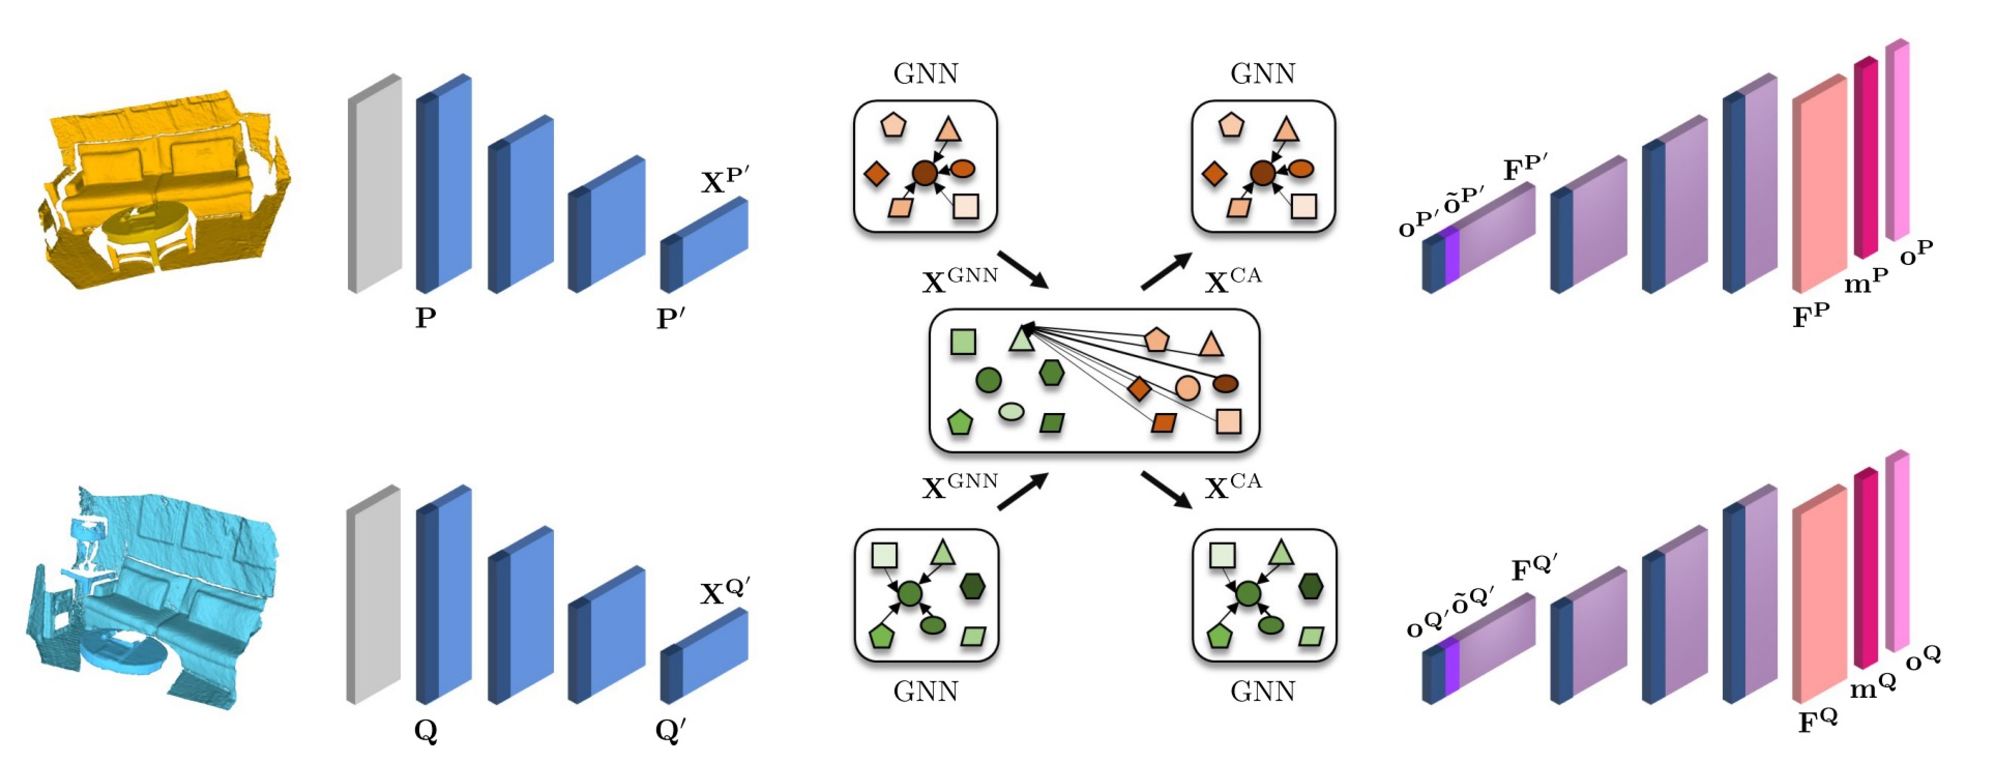
\includegraphics[width=\linewidth]{images/Predator.pdf}
    \caption{
        PREDATOR 的网络结构。体素化的点云 P 和 Q 被送入编码器,它提取出超点 P′ 和 Q′ 及其潜在特征 $\boldsymbol{X_{P'}}$ 和 $\boldsymbol{X_{Q'}}$。重叠注意力模块在一系列自我(GNN)和交叉注意力(Cross Attention)块中,更新特征的共同语境信息,并将它们投影到重叠度 $\boldsymbol{o_{P'}}$、$\boldsymbol{o_{Q'}}$ 和交叉重叠度 $\boldsymbol{\tilde{o}{P'}}$、$\boldsymbol{\tilde{o}{Q'}}$ 的得分。最后,解码器将条件特征和重叠度得分转换为每点特征描述符 $\boldsymbol{F_{P}}$、$\boldsymbol{F_{Q}}$,重叠度得分 $\boldsymbol{o_{P}}$、$\boldsymbol{o_{Q}}$,以及匹配度得分 $\boldsymbol{m_{P}}$、$\boldsymbol{m_{Q}}$。}
    \label{fig:predator}
    \vspace{-5mm}
\end{figure}

Predator\cite{huang2021predator}是一种低重叠度的三维点云配准方法,如图\ref{fig:predator}所示,Predator的架构可以分解为三个主要模块:

1. 将两个点云编码为更小的超点集合和相关的潜在特征编码,权重共享;

2. 重叠注意力模块(在瓶颈中)提取两个点云的特征编码之间的共同语境信息,并为每个超点分配两个重叠得分,这两个得分量化了超点本身和其软对应点位于两个输入之间的重叠区域的可能性;

3. 将相互调节的瓶颈表示解码为点对点描述符以及精化的每点重叠和匹配度得分。

\subsubsection{特征编码}使用大小为 V 的体素网格滤波器对原始点云进行下采样,使得 $\boldsymbol{P}$ 和 $\boldsymbol{Q}$ 具有相当均匀的点密度。在共享编码器中,一系列类似于ResNet的块和跨步卷积将原始点聚合到超点 $\boldsymbol{P' \in R^{N' \times 3}}$ 和 $\boldsymbol{Q' \in R^{M' \times 3}}$,以及相关特征 $\boldsymbol{X_{P'} \in R^{N' \times b}}$ 和 $\boldsymbol{X_{Q'} \in R^{M' \times b}}$。需要注意的是,超点对应于固定的接收场,因此它们的数量取决于输入点云的空间范围,并且对于两个输入可能是不同的。

首先,我们使用大小为 $V$ 的体素网格滤波器对原始点云进行下采样,使得 $\boldsymbol{P}$ 和 $\boldsymbol{Q}$ 具有相当均匀的点密度。在共享编码器中,一系列类似于ResNet的块和跨步卷积将原始点聚合到超点 $\boldsymbol{P' \in R^{N' \times 3}}$ 和 $\boldsymbol{Q' \in R^{M' \times 3}}$,以及相关特征 $\boldsymbol{X_{P'} \in R^{N' \times b}}$ 和 $\boldsymbol{X_{Q'} \in R^{M' \times b}}$。需要注意的是,超点对应于固定的接收场,因此它们的数量取决于输入点云的空间范围,并且对于两个输入可能是不同的。

到目前为止,瓶颈中的特征 $\boldsymbol{X_{P'}}$ 和 $\boldsymbol{X_{Q'}}$ 编码了两个点云的几何形状和上下文。但是,$\boldsymbol{X_{P'}}$ 对点云 Q 一无所知,反之亦然。为了推理它们各自的重叠区域,需要进行一些交叉对话。我们认为,在瓶颈中的超点级别添加这种交叉对话是有意义的,就像人类操作员首先会粗略地了解整体形状以确定可能的重叠区域,然后才会在这些区域中识别出精确的特征点。

图卷积神经网络:在连接两个特征编码之前,我们首先使用图神经网络(GNN)进一步聚合并强化它们各自的上下文关系。首先,使用 k-NN 方法将 $\boldsymbol{P'}$ 中的超点链接成一个欧几里得空间图。设 $\boldsymbol{x_i \in R^b}$ 表示超点 $\boldsymbol{p'_i}$ 的特征编码,$\boldsymbol{(i, j) \in E}$ 表示超点 $\boldsymbol{p'_i}$ 和 $\boldsymbol{p'_j}$ 之间的图边。然后,编码器特征按照以下方式迭代更新:
\begin{equation}
    (k+1)\boldsymbol{x_i} = \max_{(i,j) \in E} h_{\theta} \left[ \text{cat} \left[(k)\boldsymbol{x_i}, (k)\boldsymbol{x_j} - (k)\boldsymbol{x_i} \right] \right]
\end{equation}

这个更新操作执行两次,参数 $\boldsymbol{\theta}$ 并未共享,最终的 GNN 特征 $\boldsymbol{x_{GNN_i} \in R^{d_b}}$ 如下所得:

\begin{equation}
\boldsymbol{x_{GNN_i}} = h_{\theta}(\text{cat}[^{(0)}\boldsymbol{x_i}, ^{(1)}\boldsymbol{x_i}, ^{(2)}\boldsymbol{x_i}])
\end{equation}
其中,$h_{\theta}(·)$ 表示一个线性层,后面跟着实例归一化和 LeakyReLU 激活函数。

上述描述的 GNN 是针对点云 $\boldsymbol{P'}$ 的。对于 $\boldsymbol{Q'}$ 的 GNN 是相同的。

\subsubsection{交叉注意力机制}首先,将点云 $\boldsymbol{P'}$ 中的每个超点连接到 $\boldsymbol{Q'}$ 中的所有超点,形成一个二分图。受到Transformer架构的启发,我们使用向量值查询 $\boldsymbol{s_i \in R^b}$ 来根据其键 $\boldsymbol{k_j \in R^b}$ 检索其他超点的值 $\boldsymbol{v_j \in R^b}$,其中:

\begin{equation}
\begin{aligned}
\boldsymbol{k_j} &= \boldsymbol{W_k x_{GNN_j}} \\
\boldsymbol{v_j} &= \boldsymbol{W_v x_{GNN_j}} \\
\boldsymbol{s_i} &= \boldsymbol{W_s x_{GNN_i}}
\end{aligned}
\end{equation}

这里,$\boldsymbol{W_k}$, $\boldsymbol{W_v}$ 和 $\boldsymbol{W_s}$ 是可学习的权重矩阵。消息计算为值的加权平均,

\begin{figure}
    \vspace{-5mm}
    \centering
    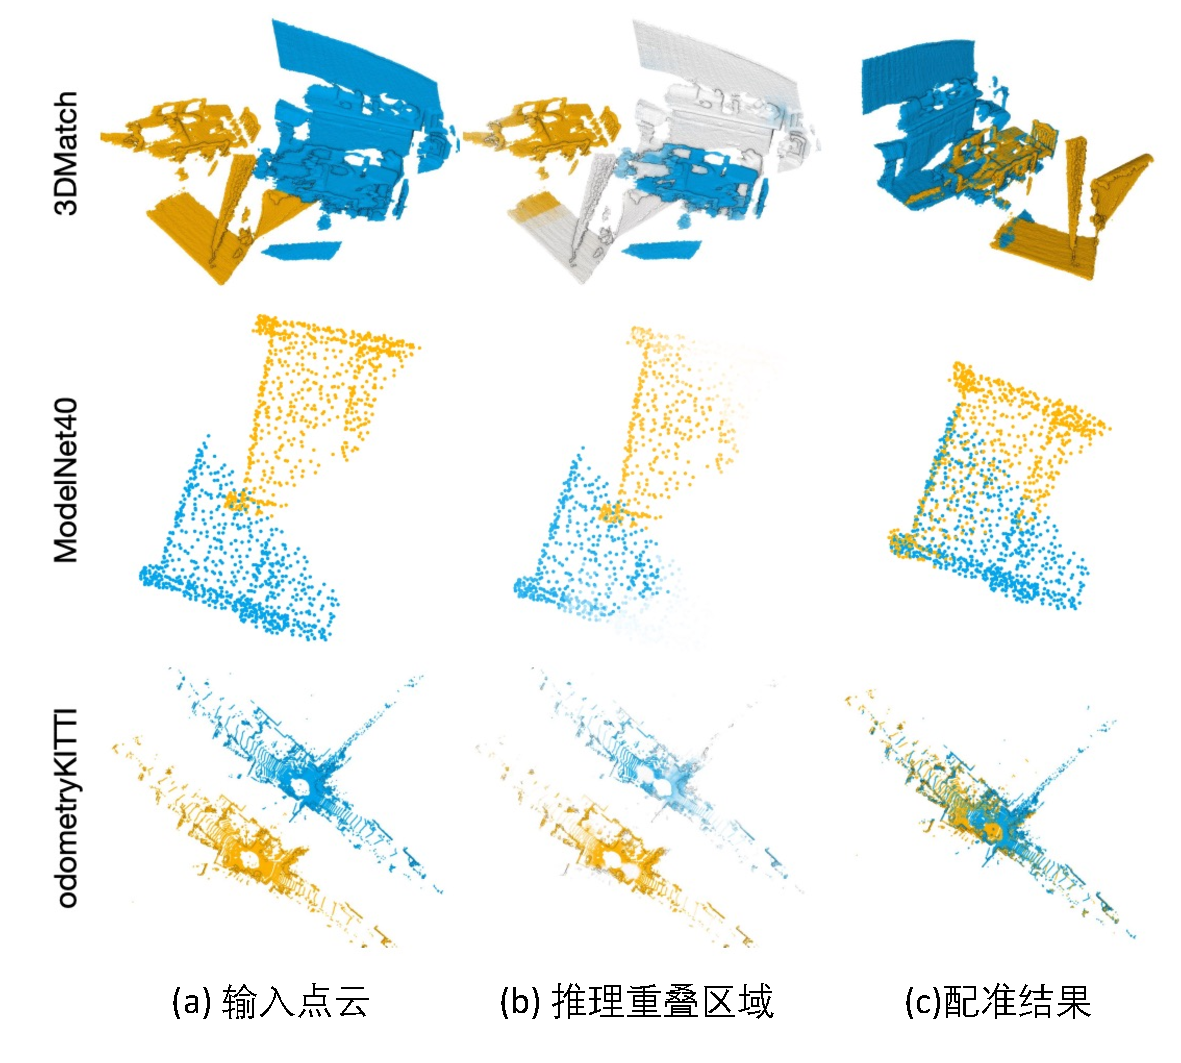
\includegraphics[width=0.6\linewidth]{images/PREDATOR_results.pdf}
    \caption{
        Predator配准示例结果。}
    \label{fig:predator_results}
    \vspace{-5mm}
\end{figure}

\begin{equation}
\boldsymbol{m_{i \leftarrow}} = \sum_{j:(i,j)\in E} a_{ij}\boldsymbol{v_j}
\end{equation}

其中注意力权重 $a_{ij} = \text{softmax}(\boldsymbol{s_i^T k_j}/\sqrt{b})$。也就是说,为了更新超点 $\boldsymbol{p'_i}$,将该点的查询与所有超点 $\boldsymbol{q'_j}$ 的键和值相结合。与文献一致,实际上我们使用具有四个并行注意力头的多注意力层。共同上下文特征计算为

\begin{equation}
\boldsymbol{x_{CA_i}} = \boldsymbol{x_{GNN_i}} + \text{MLP}(\text{cat}[\boldsymbol{s_i}, \boldsymbol{m_{i \leftarrow}}])
\end{equation}

其中 MLP(·) 表示一个三层全连接网络,在第一二层后有实例归一化和ReLU激活函数。相同的交叉注意块也反向应用,使信息在两个方向上流动,$\boldsymbol{P'} \rightarrow \boldsymbol{Q'}$ 和 $\boldsymbol{Q'} \rightarrow \boldsymbol{P'}$。

\subsubsection{瓶颈点的重叠得分}
以上更新共同上下文信息是针对每个超点单独进行的,没有考虑每个点云内的局部上下文。因此,在交叉注意块后,我们使用另一个具有相同架构和底层图(点云内链接)的 GNN 显式更新局部上下文,但参数$\theta$是独立的。这产生了最终的潜在特征编码 $\boldsymbol{F_{P'} \in R^{N' \times b}}$ 和 $\boldsymbol{F_{Q'} \in R^{M' \times b}}$,现在它们是基于其他点云特征的条件。这些特征被线性投影到重叠分数 $\boldsymbol{o_{P'} \in R^{N'}}$ 和 $\boldsymbol{o_{Q'} \in R^{M'}}$,这可以被解释为一个特定超点位于重叠区域的概率。此外,可以计算超点之间的软对应关系,并从对应关系权重预测超点 $\boldsymbol{p'_i}$ 的交叉重叠分数,即其在 $\boldsymbol{Q'}$ 的对应点位于重叠区域的概率:

\begin{equation}
\begin{aligned}
    \label{eq:soft}
\boldsymbol{\tilde{o}{P'i}} & := \boldsymbol{w_i^T o{Q'}}, \
\boldsymbol{w{ij}} & := \text{softmax} \left( \frac{1}{t} \left<\boldsymbol{f_{P'i}}, \boldsymbol{f{Q'_j}}\right> \right),
\end{aligned}
\end{equation}

其中 $\left<\cdot, \cdot\right>$ 是内积,$t$ 是控制软分配的温度参数。在 $t \rightarrow 0$ 的极限下,公式 \ref{eq:soft} 收敛到硬最近邻分配。

\subsubsection{解码器}
我们的解码器从条件特征 $\boldsymbol{F_{P'}}$ 开始,将其与重叠分数 $\boldsymbol{o_{P'}}$ 和 $\boldsymbol{\tilde{o}_{P'}}$ 连接,并输出每点特征描述符 $\boldsymbol{F_P \in R^{N \times 32}}$ 和每点的重叠分数和匹配性得分 $\boldsymbol{o_P, m_P \in R^N}$。匹配性可以被视为“条件显著性”,量化了给定另一个点云 $\boldsymbol{Q}$ 中的点(或特征)时,一个点正确匹配的可能性。

解码器的架构将NN上采样与线性层相结合,并包括来自相应编码器层的跳跃连接。我们有意将重叠得分和匹配性分开,以便解开一个点是好的/坏的匹配候选的原因:原则上,一个点可以被明确地匹配,但位于重叠区域之外,或者它可以位于重叠区域,但具有模糊的描述符。经验上,我们发现网络学习预测高匹配性主要是在重叠区域的点,这可能反映出用于训练的真实对应关系,总是在重叠区域内。结果如图 \ref{fig:predator_results} 所示。

\subsubsection{损失函数}
Predator采用端到端的训练,使用三种与地面真实对应关系相关的损失作为监督。

环形损失:为了监督点特征描述符,我们遵循[3]并使用环形损失[34],这是更常见的三元损失的一种变体。考虑一对重叠点云P和Q,这次与地面真实变换对齐。我们首先提取P中的点$\boldsymbol{p_i} \in \boldsymbol{P_p} \subset \boldsymbol{P}$,该点在Q中至少有一个(可能是多个)对应点,其中对应点集$\boldsymbol{E_p(p_i)}$定义为Q中在$\boldsymbol{p_i}$周围半径$r_p$内的点。同样,Q中所有在半径$r_s$(较大)之外的点形成负面集$\boldsymbol{E_n(p_i)}$。然后从$\boldsymbol{P_p}$中随机抽取$n_p$个点计算环形损失:
\begin{equation}
\boldsymbol{L_P^c} = \frac{1}{n_p} \sum_{i=1}^{n_p} log\left(1 + \sum_{j \in E_p} e^{\beta_j^p(d_j^i - \Delta_p)} \cdot \sum_{k \in E_n} e^{\beta_k^n(\Delta_n - d_k^i)}\right),
\end{equation}
其中$\boldsymbol{d_j^i} = ||\boldsymbol{f_{p_i}} - \boldsymbol{f_{q_j}}||_2$表示特征空间中的距离,$\Delta_n$和$\Delta_p$分别为负面和正面边距。权重$\beta_j^p = \gamma(d_j^i - \Delta_p)$和$\beta_k^n = \gamma(\Delta_n - d_k^i)$分别针对每个正面和负面例子确定,使用经验边距$\Delta_p := 0.1$和$\Delta_n := 1.4$以及超参数$\gamma$。以相同的方式计算反向损失$\boldsymbol{L_Q^c}$,总的环形损失为$\boldsymbol{L_c} = \frac{1}{2} (\boldsymbol{L_P^c} + \boldsymbol{L_Q^c})$。

重叠损失:重叠概率的估计被视为二元分类并使用重叠损失$\boldsymbol{L_o} = \frac{1}{2} (\boldsymbol{L_P^o} + \boldsymbol{L_Q^o})$进行监督,其中
\begin{equation}
\boldsymbol{L_P^o} = \frac{1}{|P|} \sum_{i=1}^{|P|} o_{p_i} log(o_{p_i}) + (1 - o_{p_i}) log(1 - o_{p_i}).
\end{equation}

点$\boldsymbol{p_i}$的地面真实标签$\boldsymbol{o_{p_i}}$定义为
\begin{equation}
\boldsymbol{o_{p_i}} =
\begin{cases}
1, & \text{if } ||\boldsymbol{T_{Q}^{P}(p_i)} - \text{NN}(\boldsymbol{T_{Q}^{P}(p_i)}, Q)||_2 < r_o \\
0, & \text{otherwise},
\end{cases}
\end{equation}
其中$r_o$为重叠阈值。反向损失$\boldsymbol{L_Q^o}$以相同方式计算。正面和负面例子的贡献通过与其相对频率成反比的权重进行平衡。

可匹配性损失:监督可匹配性得分更为困难,因为预先并不清楚在对应关系搜索中应该考虑哪些正确的点。我们遵循一个简单的直觉:好的关键点是那些在训练期间在给定点可以成功匹配的点,使用当前的特征描述符。因此,我们将预测视为二元分类并即时生成地面真实标签。再次,我们将两个对称损失求和,$\boldsymbol{L_m} = \frac{1}{2} (\boldsymbol{L_P^m} + \boldsymbol{L_Q^m})$,其中
\begin{equation}
\boldsymbol{L_P^m} = \frac{1}{|P|} \sum_{i=1}^{|P|} m_{p_i} log(m_{p_i}) + (1 - m_{p_i}) log(1 - m_{p_i}),
\end{equation}
地面真实标签$m_{p_i}$通过在特征空间中进行最近邻搜索NNF(·, ·)即时计算:
\begin{equation}
\boldsymbol{m_{p_i}} =
\begin{cases}
1, & \text{if } ||\boldsymbol{T_{Q}^{P}(p_i)} - \text{NNF}(\boldsymbol{p_i}, Q)||_2 < r_m \\
0, & \text{otherwise}.
\end{cases}
\end{equation}

\section{实验结果与分析}
本文
\subsection{PointNet}
\subsection{PointNet++}
\subsection{Predator}

\section{小结}
本章我们简要介绍了本文所使用的数据集,和点云配准评价指标。然后围绕基于深度学习的点云配准层层递进,由深度学习的基础知识介绍到了目前最常用的深度学习点云处理模型PointNet, PointNet++和Predator。后面,我们会使用预训练的PointNet和Predator作为点云特征提取器,对于描述子进行后处理。
\chapter{基于深度学习的多实例点云配准}
现有的工作主要集中在单对单的物体或场景同级别的点云配准,该方向上的工作已经十分成熟,传统的ICP配准方法\cite{barath2021progressive, li2020evaluation, shi2020improved}和深度学习方法\cite{qin2022geometric,barath2019progressive,barath2021progressive}都能达到很好的效果。但是,目前的工作对于物体对场景中多个物体的不同级别的多个配准表现仍然有待提升。本文主要构建了一种基于对应聚类方法的多实例点云配准模型和一种基于对比学习的多实例点云配准模型,将在本章展开讨论。
\section{问题陈述}

在多实例点云配准问题中,源点云$\mathbf{X}$提供了一个3D模型的实例,目标点云$\mathbf{Y}$包含了这个模型的$K$个实例,其中这些实例是一组点的集合,这些点可能只采样了3D模型的一部分。如果我们将第$k^{th}$个实例写为$\mathbf{Y}_k$,那么目标点云$\mathbf{Y}$可以分解为$
%\begin{equation}
\mathbf{Y} = \mathbf{Y}_0 \cup \mathbf{Y}_1 \cup \ldots \mathbf{Y}_k \ldots \cup \mathbf{Y}_K$。
%\end{equation}
这里我们使用$\mathbf{Y}_0$表示点云中不属于任何实例的部分。
多实例3D配准的目标是找到刚性变换$(\mathbf{R}_k, \mathbf{t}_k)$,将源实例$\mathbf{X}$对准到每个目标实例$\mathbf{Y}_k$。
如果我们设法获得源实例与每个目标实例$\mathbf{X} \leftrightarrow \mathbf{Y}_k$之间的对应关系,那么通过最小化对齐误差之和(\ref{eq:solve_rigid_transform}) \cite{SVD},可以从对应关系集合$\mathbf{X}\leftrightarrow \mathbf{Y}_k$中求解目标点云中第$k^{th}$个实例的位姿$(\mathbf{R}_k, \mathbf{t}_k)$:
\begin{equation}
\underset{\mathbf{R}_k,\mathbf{t}k}{\min}\sum_i{\parallel}\mathbf{y}{ki}-(\mathbf{R}_k\mathbf{x}_i+\mathbf{t}_k)\parallel ^2.
\label{eq:solve_rigid_transform}
\end{equation}
考虑到我们已经获得了源点云和目标点云之间的一组对应关系$\mathcal{C}$。多实例配准任务的关键是将这些对应关系分类为与不同实例相关的独立集合,即:
\begin{equation}
\mathcal{C} = \mathcal{C}_0 \cup \mathcal{C}_1\cdots \cup \mathcal{C}_K.
\end{equation}
这里,$\mathcal{C}_0$用来表示异常值集合。如我们所见,多实例配准不仅需要剔除异常值对应关系,还需要解决来自不同实例的对应关系的歧义。这个任务并不容易,因为所有实例看起来都一样,而且通常存在大量的异常值对应关系。

\section{高效对应聚类的多实例点云配准}

\subsection{结构模型}
我们提出的方法的概述如图\ref{fig:multicluster}所示。我们的方法以点对应关系作为输入。接着通过检查对应关系之间的距离一致性来构建一个不变性一致性矩阵。然后,通过将列或行向量视为这些对应关系的“特征”,将这些对应关系快速聚类成不同的组。通过凝聚聚类方法高效地进行聚类,然后通过交替合并相似的变换和重新分配簇标签进行多次迭代来进一步优化。在对应关系数量较大的情况下,我们可以选择性地应用降采样和上采样过程。详细内容将在接下来的章节中介绍。

\begin{figure*}[ht]
    \centering
    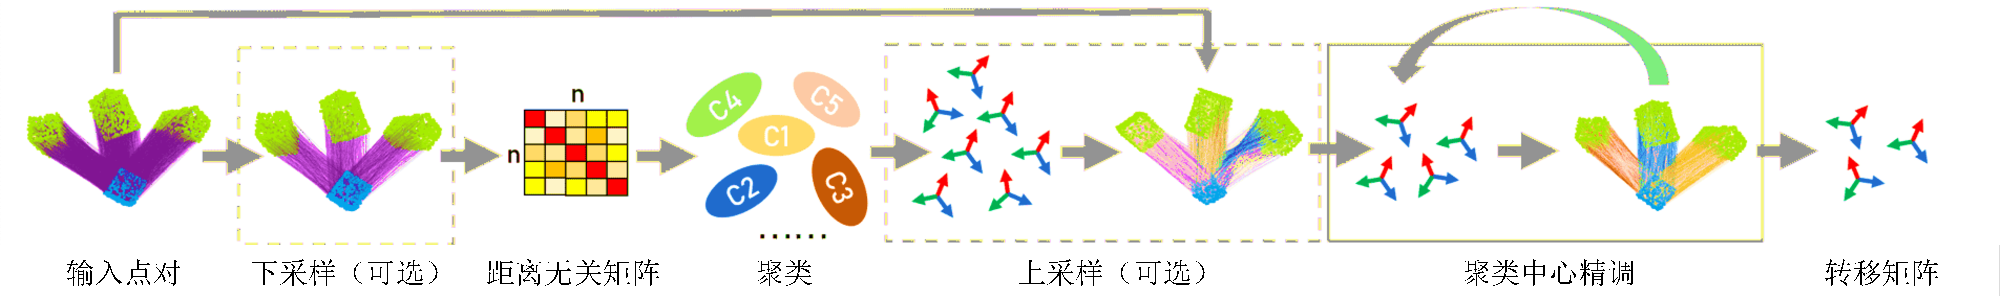
\includegraphics[width=1\textwidth]{images/multi-cluster.pdf} % Reduce the figure size so that it is slightly narrower than the column. Don't use precise values for figure width.This setup will avoid overfull boxes.
    \caption{我们提出的多实例点云配准方法的流程。从输入对应关系构建距离不变性矩阵,用于将对应关系聚类为不同的簇(\textbf{聚类}),并进行优化(\textbf{簇优化})。最后,从每个对应关系簇中估计与每个实例相关的刚体变换(\textbf{变换})。为了处理大量的对应关系,采用两个附加过程(\textbf{下采样}和\textbf{上采样})。}
    \label{fig:multicluster}
    \vspace{-0.6in}
\end{figure*}

\subsection{基于不变型矩阵的聚类}
\label{subsec:Distance-Consistency-Graph}
距离不变性特性在3D配准领域已经被研究多年\cite{yang2020teaser, shi2021robin,leordeanu2005spectral},该特性描述了在刚性变换之后两点之间的距离保持不变。具体来说,如果 $c_i :\mathbf{x}_i \leftrightarrow \mathbf{y}_i$ 和 $c_j : \mathbf{x}_j \leftrightarrow \mathbf{y}_j$ 是两个真实的对应关系,那么它们应该满足
%
\begin{equation}
G_{ij}=|d_{ij} - d'_{ij} | < \delta
\label{eq:abs_diff}
\end{equation}
其中 $d_{ij} = |\mathbf{x}_i-\mathbf{x}_j|, d'{ij}=|\mathbf{y}_i -\mathbf{y}_j|$,$\delta $ 是一个用于考虑噪声的阈值。
因此,$d_{ij}$ 和 $d'_{ij}$ 之间的差异可以用作度量是否存在异常值,或者两个对应关系是否来自不同的刚性变换的指标。我们参考\cite{matrix},使用相对差异作为度量,而不是在(\ref{eq:abs_diff})中定义的绝对差异,
\begin{equation}
G_{ij} = s_{ij}^2, s_{ij} = \min( \frac{d_{ij}}{d'_{ij}}, \frac{d'_{ij}}{d_{ij}}) \in (0, 1).
\end{equation}
通过计算所有对应关系对之间的分数,可以获得一个\emph{距离不变性矩阵} $G$(我们令 $G_{ii} = 1$)。距离不变性矩阵是对称的,其中每一列或行是一个向量,描述了给定对应关系与其他对应关系之间的兼容性\cite{reviewof3dourlierremovingjiaqiYang}。

我们将列向量 $G_i = (G_{i1}, \ldots , G_{ij}, \ldots)^T$ 称为对应关系 $c_i$ 的\emph{兼容性向量}。
我们观察到,如果两个对应关系属于同一个实例,它们的\emph{兼容性向量}具有相似的模式。
考虑两个对应关系 $c_i, c_j \in \mathcal{C}s$。对于任何对应关系 $c_k \in \mathcal{C}s$,由于距离不变性,我们有 $G_{ik} \rightarrow 1, G_{jk} \rightarrow 1$。对于其他对应关系 $c_k \in \mathcal{C}/\mathcal{C}s$,我们可能有 $G_{ik} \rightarrow 0, G_{jk} \rightarrow 0$。换句话说,$G_i,G_j$ 具有相似的 $0-1$ 模式。
相比之下,如果两个对应关系属于不同的实例,它们的兼容性向量则非常不同。

对应关系的兼容性向量可以被视为该对应关系的特征表示或“特征”。属于同一刚性变换的对应关系具有相似的特征。因此,基于这些兼容性向量,我们可以将对应关系聚类为与来自不同实例的内点相关的不同组。

\subsection{快速对应关系聚类.}
我们以自底向上的方式聚类对应关系,这比现有方法采用的谱聚类\cite{parra2019practical}\cite{shi2021robin}要快得多。一开始,每个对应关系被视为一个独立的组。然后,我们反复合并距离最小的两个组,直到两个组之间的最小距离大于给定值($min\_dist\_thresh$)。定义组之间距离的方式产生了不同风格的算法。我们遵循\cite{Tlinkage}来定义距离。设$\mathbf{p}_i, \mathbf{p}_j$为两个组$i$和$j$的表示向量,组距离定义为
\begin{equation}
d(\mathbf{p}_i, \mathbf{p}_j)= 1-\frac{\langle \mathbf{p}_i,\mathbf{p}_j\rangle}{\parallel \mathbf{p}_i\parallel ^2+\parallel \mathbf{p}_j\parallel ^2-\langle \mathbf{p}_i,\mathbf{p}_j\rangle}.
\end{equation}
如果两个组合并,新组的表示向量更新为
$\mathbf{p}_i \leftarrow \min (\mathbf{p}_i, \mathbf{p}_j),$ 其中 $\min(\cdot)$ 表示取两个向量每个维度的最小值。
在聚类开始时,一个组(只包含一个对应关系)的表示向量设置为该对应关系的兼容性向量。

\subsection{递归簇细化.}
\label{sec:cluster_refinement}
在凝聚聚类之后,我们通过重复以下步骤来进一步优化结果,直到没有变化发生。

步骤1. 从对应关系数量大于阈值 $\alpha$ 的簇中估计刚性变换。

步骤2. 合并相似的变换。这一步将在下一节中解释。

步骤3. 为每个对应关系重新分配簇标签。将每个对应关系分配给对齐误差最小的变换。如果在所有变换中最小的对齐误差大于 $inlier\_thresh$,则将对应关系标记为异常值。

在迭代过程中,对应关系变得越来越集中,因此我们可以在步骤1中调整 $\alpha$ 以增加异常值拒绝的强度。我们在每次迭代中更新 $\alpha$ 的策略如下:
\begin{equation}
\alpha \leftarrow \min(\alpha _0\times \theta ^{n-1},\left[N/100 \right] ),
\label{eq:alpha}
\end{equation}
其中 $n$ 表示第 $n^{th}$ 次迭代,$N$ 是对应关系的数量,$\left[ \cdot \right]$ 是四舍五入运算。在我们的实验中,我们设置 $\alpha_0 = 3$ 和 $\theta = 3$。细化过程通常在我们的实验中在三次迭代内收敛,因此效率也非常高。

\subsection{合并重复变换.}
有时来自不同簇的相似变换会生成,这意味着它们可能属于同一个实例。在这种情况下,我们需要合并它们。
给定两个估计的变换 $(\mathbf{R}_1, \mathbf{t}_1)$ 和 $(\mathbf{R}_2, \mathbf{t}_2)$,我们计算每个对应关系的对齐误差,即 $e{ki} = |\mathbf{y}{i}-(\mathbf{R}k \mathbf{x}_{i} + \mathbf{t}_k)|^2, (k = 1,2)$。接下来,我们设置 $p_{ki} = 1$ 如果 $e_{ki} < inlier\_thresh$,否则 $p_{ki}=0$。因此,我们为两个变换获得两个二进制集 $P_1, P_2$。合并两个变换的条件是
\begin{equation}
IOU = |P_1 \cap P_2|/|P_1 \cup P_2| \geq 80%.
\label{eq:iou}
\end{equation}
如果满足这个条件,我们将放弃一个异常值较多的变换($p_{ki} = 0$)。然后我们根据在所有变换中对齐误差最小的一个重新为每个对应关系分配簇标签。

\subsection{从簇中提取变换.}
在聚类之后,我们需要从这些对应关系簇中提取刚性变换。由于我们不知道目标点云中真实实例的数量,因此我们需要自动选择那些内点簇。我们首先选择内点簇的元素数量大于阈值(在我们的实验中为 $10$)并从这些簇中估计变换。接下来,我们根据其内点数量按降序对变换进行排序。一个变换拥有的内点越多,它与真实实例相关联的可能性就越高。最后,我们检查内点数量在变换之间的降低比例,以及第一个变换(具有最多内点)之间的比例,通过
\begin{equation}
    \gamma_k = \#I_{k}/\#I_{0},\,\, k = 1,2,\ldots
\end{equation}

其中 $\#I_k$ 表示第 $k^{th}$ 变换的内点数量。如果 $\gamma_k <= \gamma_{thresh}$,我们忽略所有在 $k$ 之后的变换。$\gamma_{thresh}$ 可以更改以在召回和精确度之间进行权衡。

\subsection{处理大量对应关系.}
% TODO down_sample and cluster
% 1.unsample
% 为什么要downsample,downsample为什么可行
当输入对应关系的数量很大时,计算距离不变矩阵和聚类对应关系可能会变得昂贵。我们通过添加下采样和上采样过程来解决这个问题。在构建距离不变矩阵之前进行下采样过程,通过随机抽样固定数量的对应关系(在我们的实现中为 $1024$)进行进一步处理。在选定对应关系聚类之后进行上采样过程,将所有对应关系分配给现有簇。分配是通过选择对齐误差最小的变换来完成的,如第 \ref{sec:cluster_refinement} 节中的步骤3所述。

\subsection{训练细节.}
我们使用 Pytorch\cite{PyTorch} 实现我们的算法。T-linkage 和 Progressive-X 是纯 CPU 算法,而 CONSAC 是基于 GPU 的学习方法。我们在与 T-linkage 和 Progressive-X 相同的 CPU(Apple M2 Max 32GB)上运行我们的算法,并在与 CONSAC 相同的 GPU(GTX A100)上运行。我们的方法有三个参数,其中在我们的实验中设置为 $min\_dist\_thresh=0.2$, $inlier\_thresh=0.3$ and $\gamma\_thresh=0.5$。所有点云都在 $0.05m$ 体素大小中进行下采样。正如补充材料中的消融研究所示,我们的方法对参数变化不敏感。

由于一对一配准中使用的指标不能用于多实例设置,我们从检索任务中采用三个评估指标:MHR(Mean Hit Recall),MHP(Mean Hit Precision),MHF1(Mean Hit F1)。详情请见第\ref{sec:multiinstance_eval}节。

\section{基于深度学习的多实例点云配准}
\subsection{对比学习}
\subsection{网络结构}
\subsection{损失函数}
\subsection{训练过程}
\subsection{推理过程}

\section{小结}
\chapter{实验结果与分析}
本章,我们对使用点云对应聚类的方式和基于深度学习的点云配准方法来进行实验。实验的数据集分为仿真数据集和真实数据集。
\section{数据集}
\subsection{仿真数据集}
如第\ref{sec:dataset}节所述,我们从 PointNet++ \cite{qi2017pointnet++} 的预采样 Modelnet40 数据集\cite{sunmodelnet40} 生成一个仿真数据集。
我们将每个点云下采样到 $256$ 个点,并随机生成 $K$ 个变换(在我们的测试中最多为 $20$)来形成一个目标点云。目标点云也与其他物体和随机点混合,以更好地模拟真实世界的情况。

\begin{figure}
        \centering
        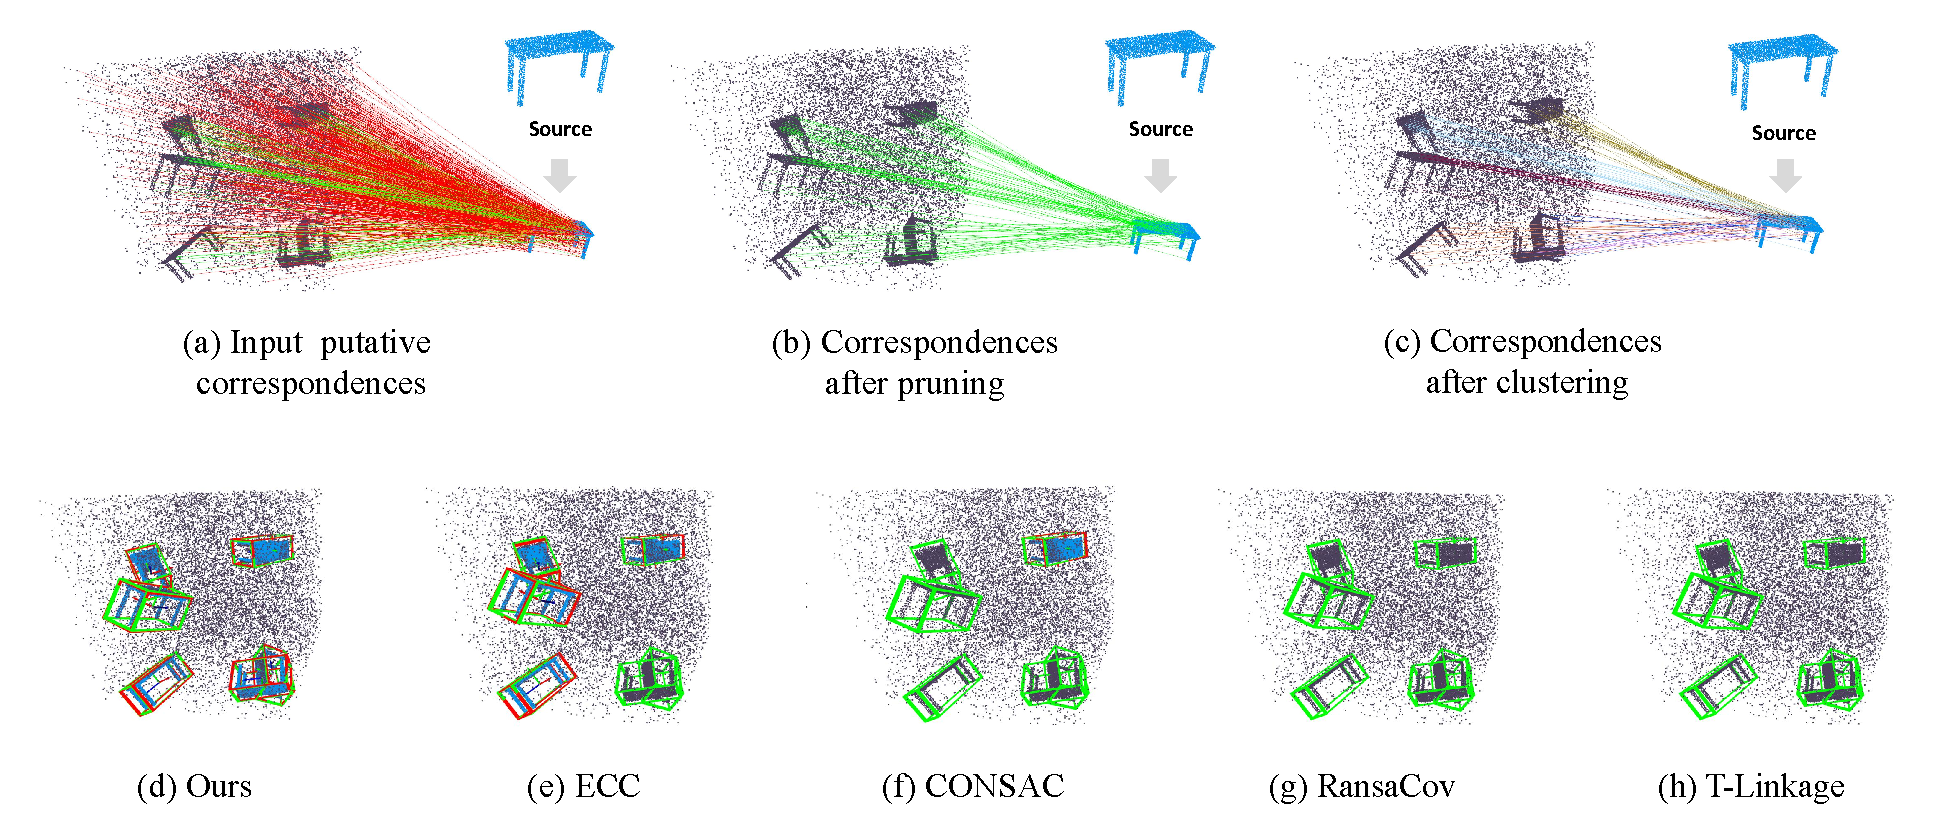
\includegraphics[width=1.0\textwidth]{images/DMR_syn.pdf}
        \caption{
                在仿真数据集上的结果。
                在 (a) 和 (b) 中,绿线和红线分别代表内点对应关系和异常值对应关系。
                在 (c) 中,聚类后每个簇中的对应关系以不同的颜色可视化。
                在 (d-f) 中,绿色边界框表示目标点云中实例的真实姿态,红色边界框表示预测。
                目标点云中的变换点云以蓝色可视化。
        }
        \label{fig:DMR}
\end{figure}

\subsection{真实数据集}
Scan2CAD\cite{avetisyan2019scan2cad} 是一个数据集,它将 ShapeNet\cite{chang2015shapenet} CAD 模型与 ScanNet\cite{dai2017scannet} 点云中的对象实例对齐。部分扫描有多个已对齐的 CAD 模型和标注的姿态。我们选择那些包含多个 CAD 模型的扫描作为目标点云,并从 CAD 模型中采样源点云进行测试。我们为配准测试生成了 173 个样本,其中大多数样本包含 $2 \sim 5$ 个实例。
请注意,在每个点云中,Scan2CAD 中仅标注了部分实例。这意味着我们无法使用部分标注的姿态正确评估性能,如准确率和召回率。为解决这个问题,我们仅在目标点云中标注的物体的真实边界框内匹配点以生成对应关系。同样,我们使用 PREDATOR\cite{huang2021predator} 和 D3Feat\cite{bai2020d3feat} 进行点匹配,两者都是使用 Scan2CAD 数据集中的 1028 个训练样本和 187 个验证样本进行微调的。

\begin{figure}[ht]
        \centering  
        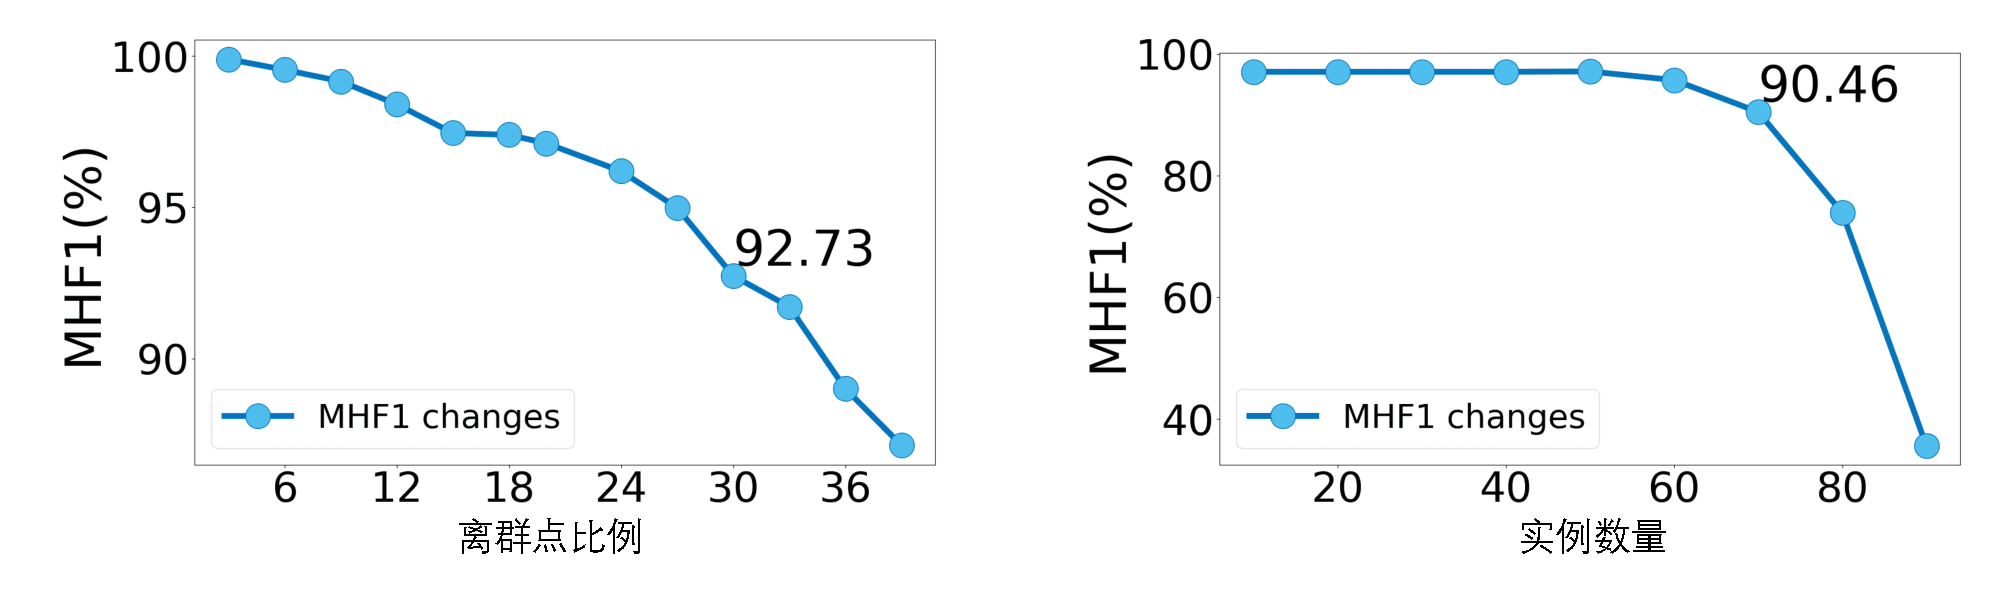
\includegraphics[width=\linewidth]{images/MHF1_curve.pdf}
        \caption{(a) 平均 Hit F1 与离群比例关系。 (b) 平均 Hit F1 与实例数量关系(固定离群比例为 $50\%$)。}
        \label{fig:detail-mm}
        %\label{fig:multi-instance}
\end{figure}

\begin{table}[h]
        \centering
        \resizebox{.75\columnwidth}{!}{
          \begin{tabular}{ccccc} %& $50\%~70\%$ & $70\%~90\%$
          \toprule
          \textbf{Metric}& MHR$\left( \% \right) \uparrow $& MHP$\left( \% \right) \uparrow $& MHF1$\left( \% \right) \uparrow $ & Time$\left( s \right) \downarrow $ \\
          \hline
          & \multicolumn{4}{c}{PREDATOR( estimated outlier ratio : $76.44\%$)} \\
          \hline
          T-Linkage & 2.46 & 3.79 & 2.71 & 1655.0 \\
          Progressive-X & 11.58 & 6.86 & 7.87 & 26.32\\
          CONSAC & 2.66 & 0.35 & 0.62 & 21.35\\
          \textbf{ECC} & \textbf{31.63} & \textbf{29.23} & \textbf{27.04} & \textbf{1.46/0.51} \\
          \hline
                          
          &\multicolumn{4}{c}{ D3Feat ( estimated outlier ratio :  $97.25\%$)} \\
          \hline
          T-Linkage & 0.04 & 0.22 & 0.06 & 2178.43 \\
          Progressive-X & \textbf{0.67} & \textbf{0.30} & \textbf{0.4} & 28.48 \\
          CONSAC & 0 & 0 & 0 & 21.88 \\
          \textbf{ECC} & 0.29 & 0.04 & 0.07 & \textbf{2.13/0.89} \\
        \bottomrule
        \end{tabular}
        }
          \caption{在Scan2CAD数据集上配准的结果。}
          \label{tab:Scan2CAD-cad}
\end{table}

\section{高效对应聚类的多实例点云配准 ECC}
\begin{figure}[ht]
        \centering  
        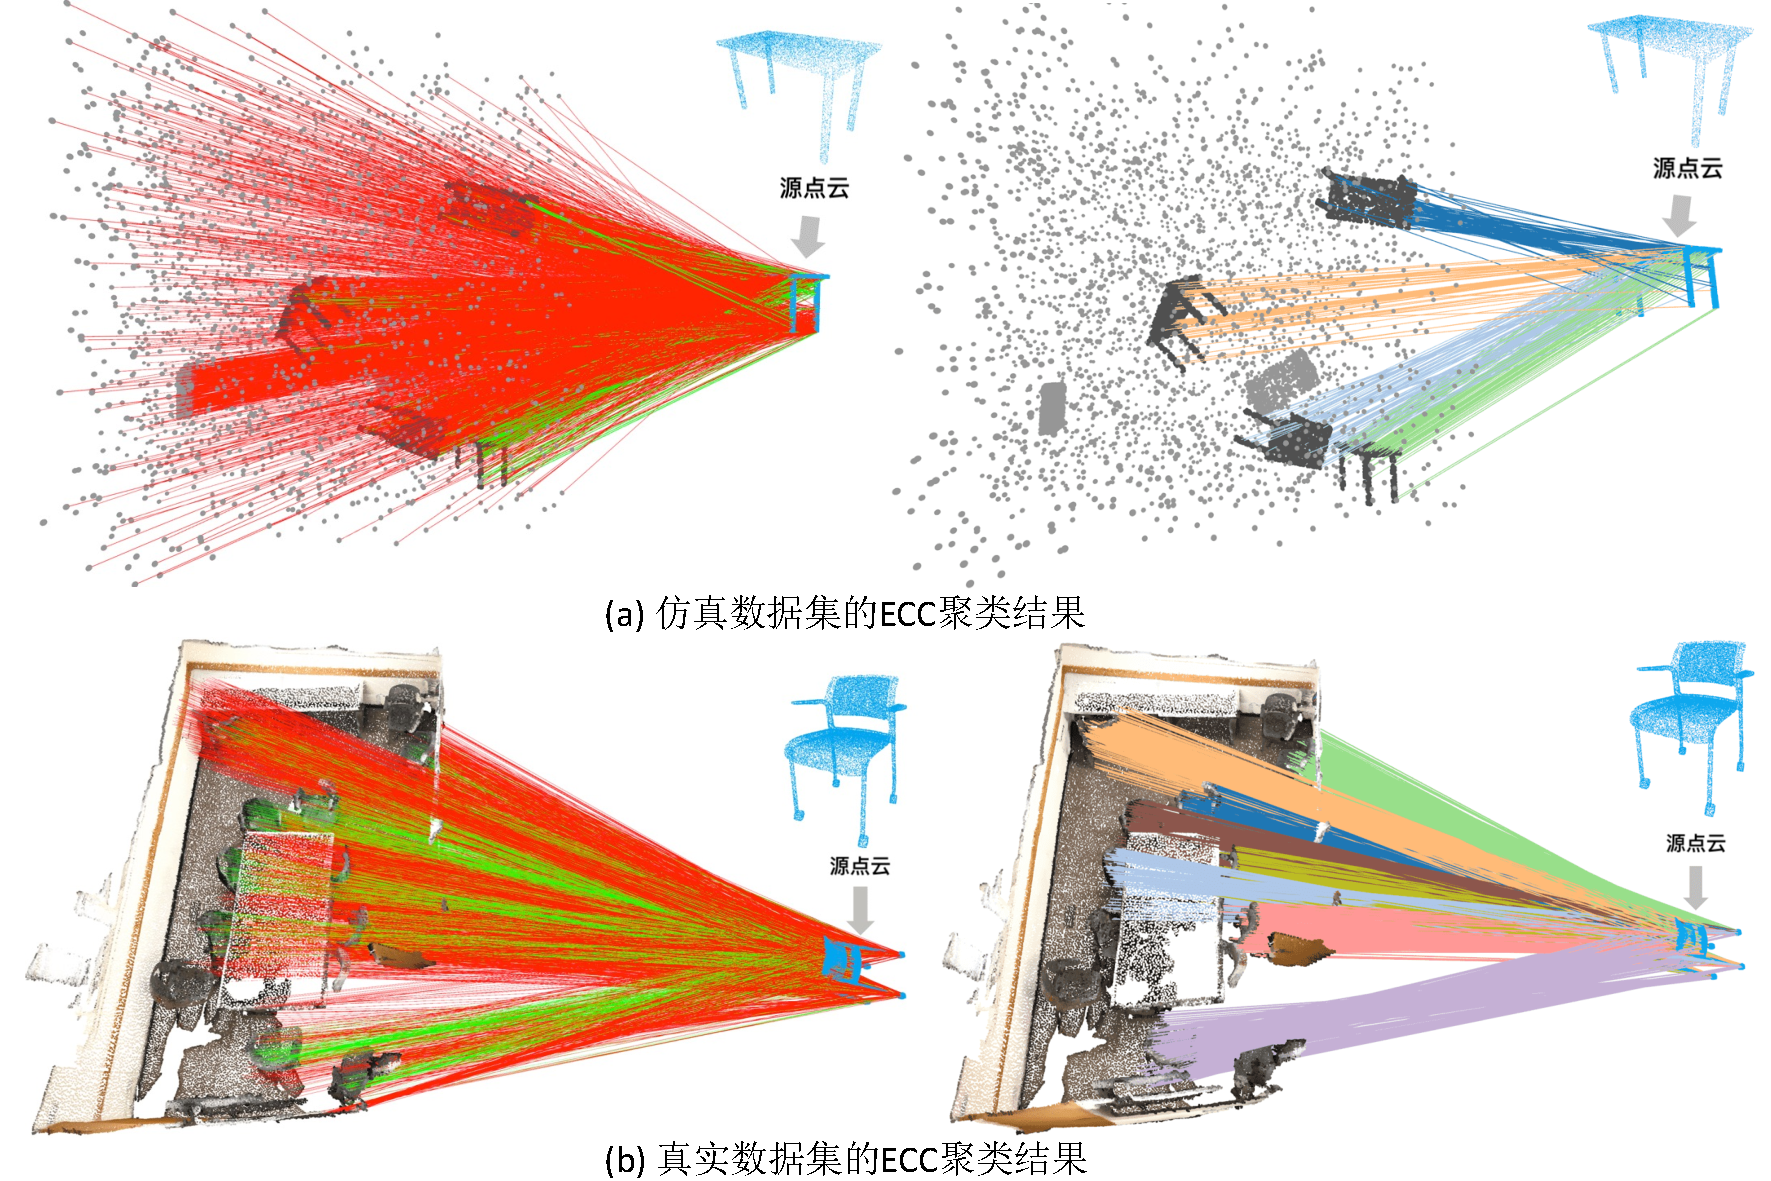
\includegraphics[width=0.75\linewidth]{images/ECC_cluster.pdf}
        \caption{ECC方法在两个数据集的聚类可视化结果}
        \label{fig:ECC_cluster}
        %\label{fig:multi-instance}
\end{figure}

\subsection{仿真数据集}
\subsubsection{仿真点对关系}
在这个测试中,我们直接通过混合真实值和离群值来生成输入对应关系。我们测试了不同的离群比例,$10\%\sim50\%$,$50\%\sim70\%$ 和 $70\%\sim90\%$。请注意,对于每个测试样本,离群点是在给定范围内随机抽样的。结果显示在表 \ref{tab:mm} 中。随着离群比例的增加,几乎所有方法的性能都有所下降,但我们的方法下降缓慢,且仍然明显优于其他方法。我们的算法在 CPU 或 GPU 上的速度比现有方法快 10 倍。
我们还在图 \ref{fig:detail-mm}(a) 中绘制了我们的方法在不同离群比例下的 MHF1(Mean Hit F1) 曲线,其中包括 $20$ 个实例。尽管当离群比例非常大时性能迅速下降,但我们的方法在 $70\%$ 的离群比例下仍然能达到 $90.46\%$ 的 MHF1。图 \ref{fig:detail-mm}(b) 显示了在固定离群比例 $50\%$ 的情况下,不同实例数量的 MHF1 曲线。即使存在 $30$ 个实例,我们的方法的 MHF1 也约为 $92.73\%$。

\subsubsection{基于特征的点对关系生成方式}

在此测试中,我们使用 PREDATOR\cite{huang2021predator} 和 D3Feat\cite{bai2020d3feat} 特征匹配来获得点对应关系。这两个特征模型都是在仿真数据上训练的。结果显示在表 \ref{tab:realcorr} 中。值得注意的是,这两个特征都产生了超过 $90\%$ 的高离群点比例。在这样一个具有挑战性的情况下,我们的方法在鲁棒性和效率方面仍然表现良好,且明显优于现有方法。使用 D3Feat 的结果要比使用 PREDATOR 的结果差得多。原因不仅是因为更多的离群点,而且我们在检查结果时发现缺少内点。在后面的实验中我们在图 \ref{fig:ECC_cluster} 中展示了一些结果。

\begin{table}[ht]
        \centering
        \resizebox{.75\columnwidth}{!}{
        \begin{tabular}{ccccc} %& $50\%~70\%$ & $70\%~90\%$
            \toprule
            % & MHR$\left( \% \right) \uparrow $ & MHRRE $\left( \right) \downarrow $ & MHRTE & Time\\
            \textbf{方法}& MHR$\left( \% \right) \uparrow $ & MHP$\left( \% \right) \uparrow $ & MHF1$\left( \% \right) \uparrow $ & 时间$\left( s \right) \downarrow $\\
            \hline
            \multicolumn{5}{c}{离群点比重 : $10\%\sim50\%$} \\
            \hline
            T-Linkage & 3.05 & 14.80 & 4.65& 57.27 \\
            Progressive-X & 27.91 & 80.28 & 41.04 & 87.25\\
            CONSAC & 0.47 & 0.47 & 0.47 & 9.23  \\
            \textbf{ECC} & \textbf{96.08} & \textbf{99.73} & \textbf{97.03} & \textbf{0.62/0.30} \\ % 前gt_num个预测值的recall
            \hline
            \multicolumn{5}{c}{离群点比重 : $50\%\sim70\%$} \\
            \hline
            %\hline
            % \textbf{metric} & MHR$\left( \% \right) \uparrow $ & RRE$\left( \degree \right) \downarrow $ & RTE$\left( m \right) \downarrow $ & t$\left( s \right) \downarrow $\\
            %\hline
            %\hline
            T-Linkage & 1.33 & 7.00 & 2.05 & 56.90 \\
            Progressive-X & 20.60 & 75.10 & 31.70 & 85.54  \\
            CONSAC & 0.49 & 0.49 & 0.49 & 9.55\\
            \textbf{ECC} & \textbf{93.99} & \textbf{99.49} & \textbf{95.51} & \textbf{0.55/0.28}\\
            \hline
            
            \multicolumn{5}{c}{Outlier ratio : $70\%\sim90\%$} \\
            \hline
            %\hline
            % \textbf{metric} & MHR$\left( \% \right) \uparrow $ & RRE$\left( \degree \right) \downarrow $ & RTE$\left( m \right) \downarrow $ & t$\left( s \right) \downarrow $\\
            %\hline
            %\hline
            T-Linkage & 0.81 & 4.42 & 1.25 & 56.89 \\
            Progressive-X & 12.88 & 62.60 & 20.73 & 84.5 \\
            CONSAC & 0.51 & 0.51 & 0.51 & 7.70  \\
            \textbf{ECC} & \textbf{60.39} & \textbf{94.42} & \textbf{69.36} &\textbf{0.50/0.24}\\
    
            \hline
            \multicolumn{5}{c}{离群点比重 : $90\%\sim99\%$} \\
            \hline
            T-Linkage & 0.28 & 1.30 & 0.42 & 56.69 \\
            Progressive-X & 7.13 & 39.19 & 11.67 & 84.43\\
            CONSAC & 0.51 & 0.51 & 0.51 & 9.57  \\
            \textbf{ECC} & \textbf{14.70} & \textbf{65.20} & \textbf{22.75} & \textbf{0.47/0.21} \\ % 前gt_num个预测值的recall
            \bottomrule
            %outlier ratio & $10\%~50\%$ & $50\%~70\%$ & $70\%~90\%$\\
    
        \end{tabular}
        }
        \caption{在不同离群比例的仿真对应关系上的结果。$\uparrow$ 表示越大越好,而 $\downarrow$ 表示相反。我们方法在 CPU/GPU 上的运行时间也展示出来。}
        \label{tab:mm}
\end{table}

\begin{table}
        \centering
        \resizebox{0.75\textwidth}{!}{
            \begin{tabular}{ccccc} 
                \toprule
                \textbf{Metric}& MHR$\left( \% \right) \uparrow $& MHP$\left( \% \right) \uparrow $& MHF1$\left( \% \right) \uparrow $ & Time$\left( s \right) \downarrow $\\
                \hline
                & \multicolumn{4}{c}{PREDATOR ( estimated outlier ratio : $94.32\%$)} \\
                \hline
                T-Linkage & 0.19 & 0.54 & 0.27 & 43.46 \\
                Progressive-X & 15.90 & 31.01 & 18.98 & 86.39 \\
                CONSAC & 0.1 & 0.07 & 0.08 & 7.65 \\
                \textbf{ECC} &\textbf{53.39} & \textbf{61.44} & \textbf{51.80} & \textbf{1.28/0.48} \\
                \hline
                
                &\multicolumn{4}{c}{D3Feat ( estimated outlier ratio : $99.30\%$)} \\
                \hline
                %\hline
                % \textbf{metric} & MHR$\left( \% \right) \uparrow $ & RRE$\left( \degree \right) \downarrow $ & RTE$\left( m \right) \downarrow $ & t$\left( s \right) \downarrow $\\
                %\hline
                %\hline
                T-Linkage & 0.07 & 0.29 & 0.1 & 56.37  \\
                Progressive-X & 4.29 & 15.28 & 5.94 & 87.22 \\
                CONSAC & 0.13 & 0.04 & 0.05 & 9.53 \\
                \textbf{ECC} & \textbf{16.98} & \textbf{27.05} & \textbf{17.91} & \textbf{0.68/0.30} \\
                \bottomrule
        \end{tabular}
        }
        \caption{使用特征匹配在仿真数据上生成对应点的结果。部分结果可在图 \ref{fig:ECC_cluster} 中进行可视化。}
        % \caption{Results on synthetic data using feature matching to generate correspondences.$\uparrow$ means the larger the better, while $\downarrow$ indicates the contrary. The running time on CPU/GPU of our method is presented. Some results are visualized in Figure \ref{fig:predatormm}.}
        \label{tab:realcorr}
\end{table}

\subsection{真实数据集}
在真实数据集中的测试结果如表 \ref{tab:Scan2CAD-cad} 所示。我们的方法在使用 PREDATOR 时明显优于现有方法。请注意,当使用 D3Feat 时,所有方法的性能都很差。在仔细检查结果后,我们发现原因不仅是高异常值比率(约 $97.25\%$),而且在使用 D3Feat 时,即使特征匹配仅限于目标点云中的真实边界框内,内点也不足。一些结果如图 \ref{fig:DMR_real}(e) 所示。


\section{基于深度学习的多实例点云配准 DMR}
\subsection{仿真数据集}
我们首先将基于深度学习的方法与仿真数据集上的其他竞争者进行比较,结果如表 \ref{table1} 所示。
由于内点比例极低,基于采样的方法如 T-Linkage、RansaCov 和 CONSAC 的性能不佳。
由于空间一致性的优势,ECC 表现出有效性。
然而,我们的 DMR 在所有评价指标上均大幅度超越了第二好的方法 ECC。

\setlength{\tabcolsep}{8pt}
\begin{table}[ht]
  \centering
  \caption{在仿真数据集上的配准结果}
  \begin{tabular}{ccccc}
    \hline\noalign{\smallskip}
  & MHR(\%)         & MHP(\%)         & MHF1(\%)         & Time(s)       \\
  \noalign{\smallskip}
  \hline
  \noalign{\smallskip}
  T-linkage  & 0.61           & 1.48           & 0.87           & 3.89          \\
  RansaCov   & 0.73           & 5.33           & 1.29           & 0.14          \\
  CONSAC     & 1.00           & 7.45           & 1.77           & 0.61          \\
  ECC         & 82.90          & 92.92          & 87.63          & 3.56          \\
  DMR              & \textbf{92.60} & \textbf{99.69} & \textbf{96.01} & \textbf{0.06} \\
  \hline
  \end{tabular}
  \label{table1}
\end{table}

为了定性评估我们的DMR并将其与其他竞争者进行比较,我们在图 \ref{fig:DMR} 中提供了一组可视化。图 \ref{fig:DMR} 的第一行显示了输入对应关系,以及我们的剪枝和聚类结果。图 \ref{fig:DMR}(b) 显示,我们的DMR惊人地去除了所有的离群点,剩余的对应关系在图 \ref{fig:DMR}(c) 中被很好地聚类。

图 \ref{fig:DMR} 的第二行显示了我们提出的方法和竞争者的配准结果。可以看到,T-Linkage和RansaCov都无法配准任何实例。对于目标点云中的六个实例,CONSAC只成功配准了一个实例。值得注意的是,尽管ECC成功配准了四个实例,但它未能配准右下角的两张桌子。这是因为这两张桌子混在一起,空间一致性不足以区分它们。然而,我们的方法成功配准了所有实例。

\subsection{真实数据集}
\begin{table}[ht]
        \centering
        \caption{在真实数据集上的配准结果}
        \begin{tabular}{ccccc}
        \hline\noalign{\smallskip}
        & MHR(\%)         & MHP(\%)         & MHF1(\%)         & Time(s)       \\
        \noalign{\smallskip}
        \hline
        \noalign{\smallskip}
        T-linkage  & 34.99          & 46.86          & 40.07          & 6.64          \\
        RansaCov   & 60.50          & 33.28          & 42.94          & \textbf{0.07} \\
        CONSAC     & 55.48          & 53.34          & 54.39          & 0.39          \\
        ECC        & 64.66          & 69.73          & 67.10          & 1.84          \\
        DMR   & \textbf{78.10} & \textbf{70.64} & \textbf{74.18} & 0.10        \\ 
        \hline
        \end{tabular}
        \label{tab:DMR_real}
\end{table}
      
如表 \ref{tab:DMR_real} 所示,我们的DMR在所有三个评估指标,MHR, MHP 和MHF 上均优于所有竞争者,速度也很有竞争力。 
ECC和DMR的性能低于仿真数据集,而其他方法的性能高于仿真数据集。 
这是由于实例内点比率分布的变化。 
      
我们还提供了一组可视化,以定性评估我们的DMR并与其他竞争者进行比较。 
图 \ref{fig:DMR_real}的第一行显示了输入对应关系,以及我们的剪枝和聚类结果。 
图 \ref{fig:DMR_real}(b)表明,我们的方法几乎去除了所有的异常值,确保了如图 \ref{fig:DMR_real}(c)所示的后续聚类高效执行。 
对于包含在目标点云中的五个实例,T-Linkage和CONSAC成功配准了两个实例,但T-Linkage的一个预测有大的错误。 
RansaCov成功配准了三个实例。 
由于目标点云中的三把椅子靠得很近,ECC并没有成功配准所有这些实例。 
我们的方法成功完成了所有实例的配准。
      
\begin{figure}
        \centering
        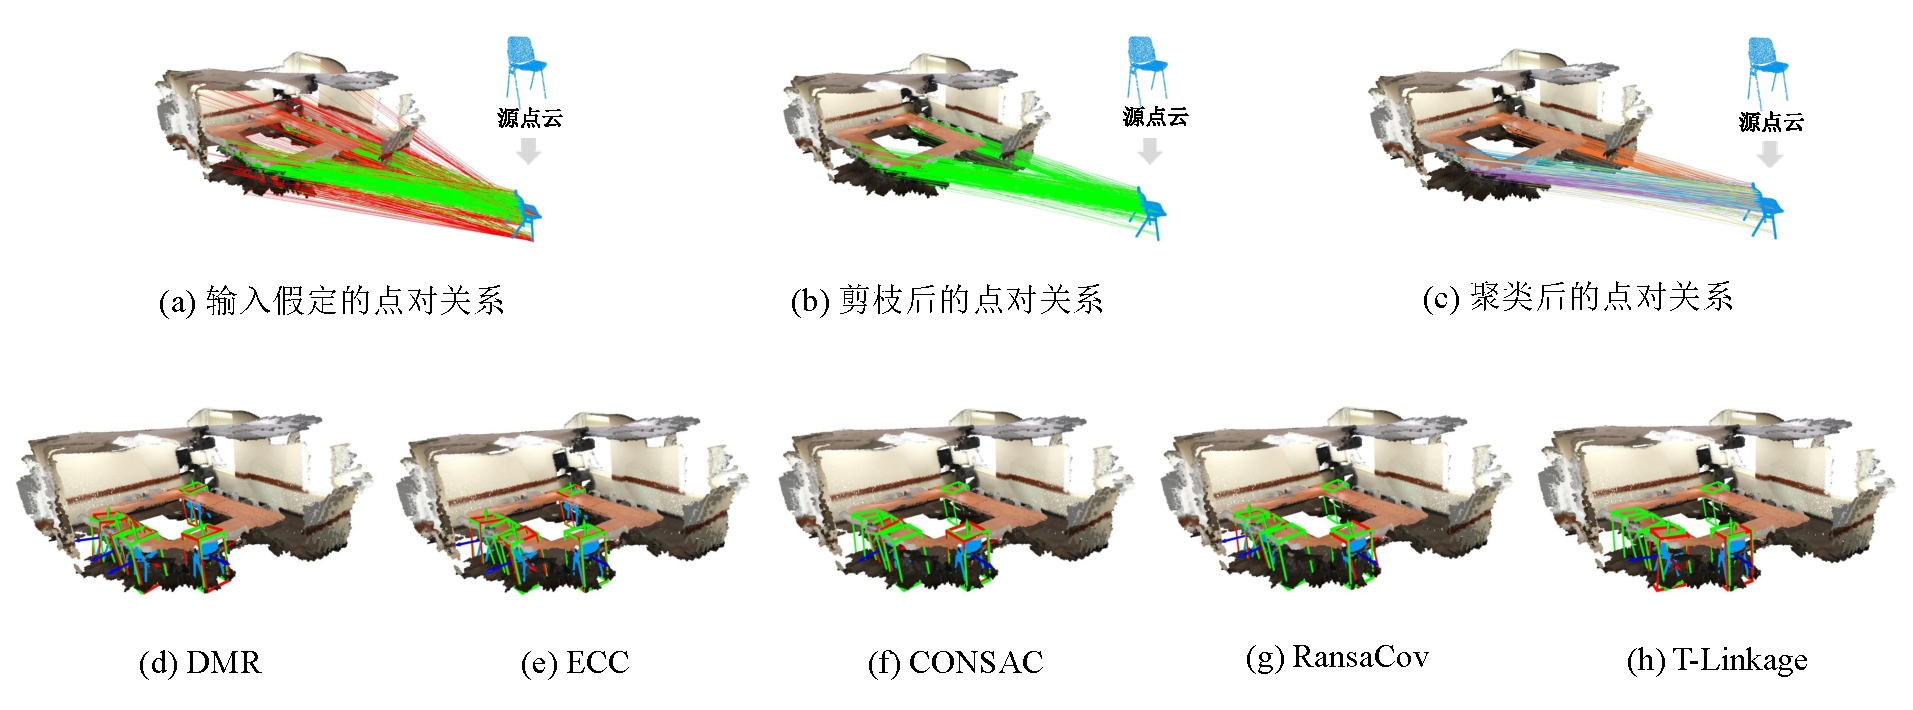
\includegraphics[width=1.0\textwidth]{images/DMR_real.pdf}
        \caption{
          在真实数据集上的结果。
          在(a)和(b)中,绿线和红线分别代表内点对应关系和异常值对应关系。
          在(c)中,聚类后每个簇中的对应关系以不同的颜色可视化。
          在(d-f)中,绿色边界框表示目标点云中实例的真实姿态,红色边界框表示预测。
          目标点云中的变换点云以蓝色可视化。
        }
        \label{fig:DMR_real}
\end{figure}
      
\subsection{消融实验}
\label{sec:ablation}
\subsubsection{深度表达的消融研究}为了研究我们采用的深度表达的有效性,我们比较了我们的框架在有和无深度表达下的性能。
没有深度表达的版本删除了特征提取器并设置 $S=\beta$,只依赖空间一致性进行剪枝和聚类。
比较结果如表 \ref{tab:ablation} 所示。
可以看到,使用深度表达后,准确性和速度指标都有所提高。
没有深度表达,剪枝的对应关系少,需要聚类的对应关系多,这增加了我们方法的运行时间。
尽管没有深度表达的框架在MHR、MHP和MHF1上的性能较低,但它仍然是一个有竞争力的基线,适合没有训练数据的情况。
这表明了本文提出的剪枝和聚类策略的有效性。

此外,我们在图 \ref{fig:spectral} 中可视化了有无深度表达的聚类结果。
我们选择了一个例子,其目标点云包含三个实例。
我们首先使用一个3维的one-hot向量来表示一个对应关系属于哪个实例。
然后我们使用这些向量来计算相似性矩阵,并使用聚类的结果对这些矩阵进行排列。
可以看到,通过深度表达排列的相似性矩阵比没有深度表达的框架排列的相似性矩阵小得多,因为在前者的情况下,剪枝过程中去除了更多的异常值。
更重要的是,图 \ref{fig:spectral}(b) 中的矩阵显示了三个明显的簇,这些簇对应于三个实例。
相反,图 \ref{fig:spectral}(a) 中的矩阵显示了两个块,其中右下角的块实际上对应于两个实例,如果不使用提出的深度表达,无法成功区分。

\setlength{\tabcolsep}{2pt}
\begin{table}
  \caption{
    深度表达和剪枝的消融研究结果。
    }
  \centering
  \begin{tabular}{cccccc}
    \hline\noalign{\smallskip}
    深度表达 & 剪枝 & MHR(\%)         & MHP(\%)         & MHF1(\%)         & Time(s)       \\
  \noalign{\smallskip}
  \hline
  \noalign{\smallskip}
  & $\checkmark$       & 76.61          & 65.05          & 70.36          & 0.17          \\
  $\checkmark$                   &         & 62.23          & 32.77          & 42.93          & 1.24          \\
  $\checkmark$                &
 $\checkmark$     & \textbf{78.10} & \textbf{70.64} & \textbf{74.18} & \textbf{0.10}\\
  \hline
  \end{tabular}
  \label{tab:ablation}
\end{table}
\setlength{\tabcolsep}{1.4pt}


\begin{figure}
  \centering
  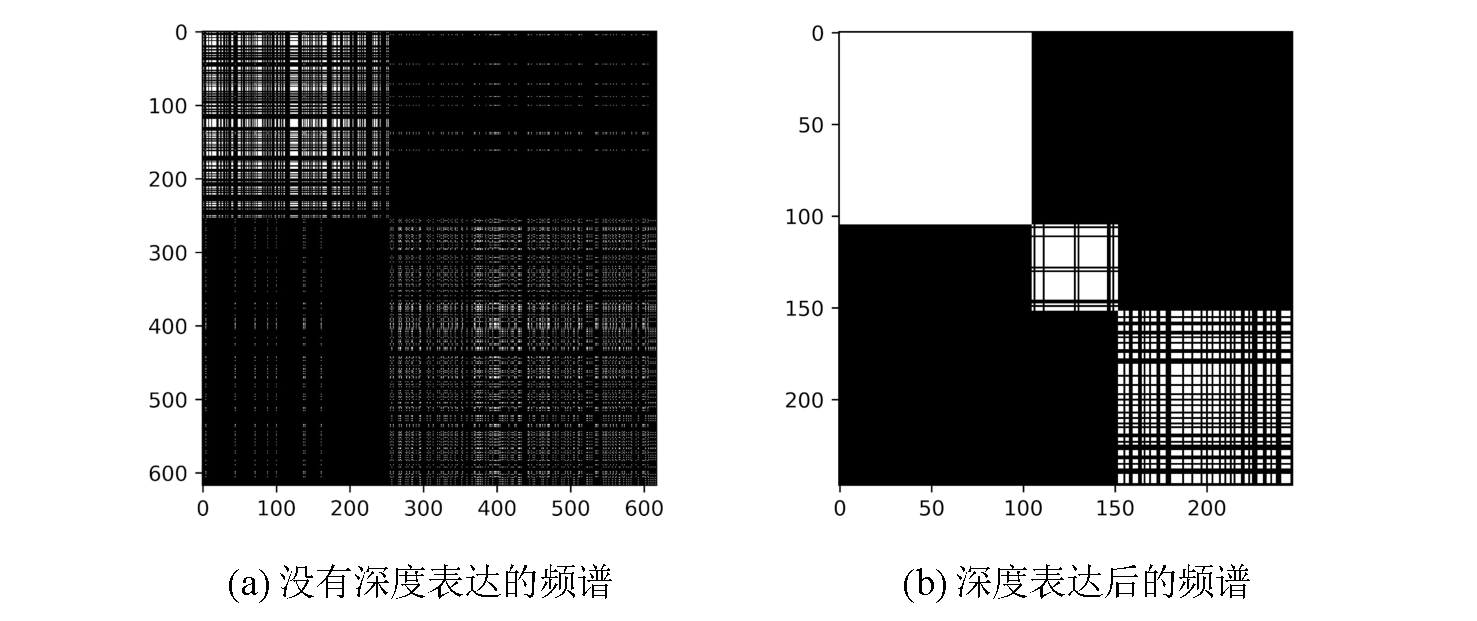
\includegraphics[width=0.8\textwidth]{images/spectral.pdf}
  \caption{
    无深度表达和有深度表达的聚类结果可视化。
    }
    \vspace{-0.5cm}
  \label{fig:spectral}
\end{figure}

\subsubsection{对剪枝的消融研究}
为了定量研究我们的剪枝策略的有效性,我们简单地在我们的方法中去除剪枝策略,然后比较去除前后的性能。
表 \ref{tab:ablation} 显示,如果去除剪枝步骤,我们的方法的性能会大幅下降,这是由于噪声二进制相似性矩阵不符合 \cite{li2007noise} 定义的理想矩阵,光谱聚类无法正确地对应关系进行分组。
这个结果表明,剪枝对后续的聚类至关重要。

\subsubsection{对 RANSAC 迭代次数的消融研究}
\vspace{-0.3cm}
此外,我们还测试了我们的模型在不同的 RANSAC 迭代次数下的性能,结果如表 \ref{tab:ransac} 所示。
可以看到,只用五次迭代就可以得到相当好的结果,而 50 次和 500 次迭代的性能非常接近。
这些结果表明,剪枝和聚类步骤极大地提高了每个实例的内点比例,因此,只使用少量的迭代次数就可以估计出可靠的结果。


\begin{table}
  \caption{
        RANSAC 迭代次数的影响
  }
  \centering
  \begin{tabular}{cccc}
    \hline\noalign{\smallskip}
    RANSAC 次数 & MHR(\%)         & MHP(\%)         & MHF1(\%)          \\
  \noalign{\smallskip}
  \hline
  \noalign{\smallskip}
  5   & 77.39          & 67.76          & 72.26              \\
  50  & 78.10          & \textbf{70.64} & 74.18                \\
  500 & \textbf{79.33} & \textbf{70.64} & \textbf{74.73}  \\  
  \hline
  \end{tabular}
  \label{tab:ransac}
\end{table}

\subsubsection{关于最难负样本消融研究}
\vspace{-0.3cm}
为每个小批量找到最困难的负对会产生更大的计算开销,但我们的消融研究显示这是值得的。
我们将其与使用随机选择的负对训练的相同模型进行比较。
使用最困难的负对(如本方法所述)和使用随机选择的负对的结果如表 \ref{tab:hardest} 所示。
所有的准确性指标都通过在对比学习中使用最困难的负对得到了提升。
通过比较表 \ref{tab:hardest} 和表 \ref{tab:ablation},我们可以发现,在对比表示学习中使用随机负对得到的结果优于不使用深度表达,但差距很小。
此外,我们在表 \ref{tab:hardest} 中收集了特征空间中正对和 top-K 最困难的负对的平均余弦相似性。
结果显示,使用最困难的负对训练的表示在特征空间中更好地分离,更具区分性。

\begin{table}
  \caption{
        用最难的负样本进行训练的消融实验结果。
  }
  \centering
  \begin{tabular}{ccccccc}
    \hline\noalign{\smallskip}
    & MHR(\%) & MHP(\%) & MHF1(\%) & Positive(\%) & Top-1(\%) & Top-10(\%) \\
    \noalign{\smallskip}
    \hline
    \noalign{\smallskip}
    随机  & 76.85  & 67.50  & 71.87  & 95.43 & 96.91 & 91.37  \\
    最难 & \textbf{78.10} & \textbf{70.64} & \textbf{74.18} & 83.96 & 61.32 & 49.65 \\  
    \hline
  \end{tabular}
  \label{tab:hardest}
\end{table}


\section{小结}
本章,我们对提出的两种多实例点云配准模型进行了广泛的实验评估,包括定量的实验评估和可视化的实验评估,并且对基于深度学习的方法进行了广泛的消融实验。其中基于深度学习的方法效果超过了单纯的聚类算法,证明了深度学习方法在多实例点云配准中的有效性,学习鲁棒的点对特征能够大大增大配准的效果。

% 后置部分
\backmatter

% 结论:在结论相应的 TeX 文件处进行结论部分的撰写
%%
% The BIThesis Template for Bachelor Graduation Thesis
%
% 北京理工大学毕业设计(论文)结论 —— 使用 XeLaTeX 编译
%
% Copyright 2020-2023 BITNP
%
% This work may be distributed and/or modified under the
% conditions of the LaTeX Project Public License, either version 1.3
% of this license or (at your option) any later version.
% The latest version of this license is in
%   http://www.latex-project.org/lppl.txt
% and version 1.3 or later is part of all distributions of LaTeX
% version 2005/12/01 or later.
%
% This work has the LPPL maintenance status `maintained'.
%
% The Current Maintainer of this work is Feng Kaiyu.
%
% Compile with: xelatex -> biber -> xelatex -> xelatex

\begin{conclusion}
  % 结论部分尽量不使用 \subsection 二级标题,只使用 \section 一级标题

  % 这里插入一个参考文献,仅作参考
\end{conclusion}


% 参考文献:如无特殊需要,参考文献相应的 TeX 文件无需改动,添加参考文献请使用 BibTeX 的格式
%   添加至 misc/ref.bib 中,并在正文的相应位置使用 \cite{xxx} 的格式引用参考文献
%%
% The BIThesis Template for Bachelor Graduation Thesis
%
% 北京理工大学毕业设计(论文)参考文献 —— 使用 XeLaTeX 编译
%
% Copyright 2020-2023 BITNP
%
% This work may be distributed and/or modified under the
% conditions of the LaTeX Project Public License, either version 1.3
% of this license or (at your option) any later version.
% The latest version of this license is in
%   http://www.latex-project.org/lppl.txt
% and version 1.3 or later is part of all distributions of LaTeX
% version 2005/12/01 or later.
%
% This work has the LPPL maintenance status `maintained'.
%
% The Current Maintainer of this work is Feng Kaiyu.
%
% Compile with: xelatex -> biber -> xelatex -> xelatex
%
% 如无特殊需要,本页面无需更改

\begin{bibprint}

% -------------------------------- 示例内容(正式使用时请删除) ------------------------------------- %

% 抑制多次调用 \printbibliography 的 warning,只有示例代码会需要此语句。
\BiblatexSplitbibDefernumbersWarningOff

% \textcolor{blue}{参考文献书写规范}

% \textcolor{blue}{参考国家标准《信息与文献参考文献著录规则》【GB/T 7714—2015】,参考文献书写规范如下:}

% \textcolor{blue}{\textbf{1. 文献类型和标识代码}}

% \textcolor{blue}{普通图书:M}\qquad\textcolor{blue}{会议录:C}\qquad\textcolor{blue}{汇编:G}\qquad\textcolor{blue}{报纸:N}

% \textcolor{blue}{期刊:J}\qquad\textcolor{blue}{学位论文:D}\qquad\textcolor{blue}{报告:R}\qquad\textcolor{blue}{标准:S}

% \textcolor{blue}{专利:P}\qquad\textcolor{blue}{数据库:DB}\qquad\textcolor{blue}{计算机程序:CP}\qquad\textcolor{blue}{电子公告:EB}

% \textcolor{blue}{档案:A}\qquad\textcolor{blue}{舆图:CM}\qquad\textcolor{blue}{数据集:DS}\qquad\textcolor{blue}{其他:Z}

% \textcolor{blue}{\textbf{2. 不同类别文献书写规范要求}}

% \textcolor{blue}{\textbf{期刊}}

% \noindent\textcolor{blue}{[序号]主要责任者. 文献题名[J]. 刊名, 出版年份, 卷号(期号): 起止页码. }

% \printbibliography [type=article,heading=none] 

% \textcolor{blue}{\textbf{普通图书}}

% \noindent\textcolor{blue}{[序号]主要责任者. 文献题名[M]. 出版地: 出版者, 出版年. 起止页码. }
% \cite{Raymer1992Aircraft}

% \printbibliography [keyword={book},heading=none] 

% \textcolor{blue}{\textbf{会议论文集}}

% \noindent\textcolor{blue}{[序号]析出责任者. 析出题名[A]. 见(英文用In): 主编. 论文集名[C]. (供选择项: 会议名, 会址, 开会年)出版地: 出版者, 出版年. 起止页码. }
% \cite{sunpinyi}

% \printbibliography [type=inproceedings,heading=none] 

% \textcolor{blue}{\textbf{专著中析出的文献}}

% \noindent\textcolor{blue}{[序号]析出责任者. 析出题名[A]. 见(英文用In): 专著责任者. 书名[M]. 出版地: 出版者, 出版年.起止页码. }
% \cite{luoyun}

% \printbibliography [type=inbook,heading=none] 

% \textcolor{blue}{\textbf{学位论文}}

% \noindent\textcolor{blue}{[序号]主要责任者. 文献题名[D]. 保存地: 保存单位, 年份. }
% \cite{zhanghesheng}
% \cite{Sobieski}

% \printbibliography [keyword={thesis},heading=none] 

% \textcolor{blue}{\textbf{报告}}

% \noindent\textcolor{blue}{[序号]主要责任者. 文献题名[R]. 报告地: 报告会主办单位, 年份. }
% \cite{fengxiqiao}
% \cite{Sobieszczanski}

% \printbibliography [keyword={techreport},heading=none] 

% \textcolor{blue}{\textbf{专利文献}}

% \noindent\textcolor{blue}{[序号]专利所有者. 专利题名[P]. 专利国别: 专利号, 发布日期. }
% \cite{jiangxizhou}

% \printbibliography [type=patent,heading=none] 

% \textcolor{blue}{\textbf{国际、国家标准}}

% \noindent\textcolor{blue}{[序号]标准代号. 标准名称[S]. 出版地: 出版者, 出版年. }
% \cite{GB/T16159—1996}

% \printbibliography [keyword={standard},heading=none] 

% \textcolor{blue}{\textbf{报纸文章}}

% \noindent\textcolor{blue}{[序号]主要责任者. 文献题名[N]. 报纸名, 出版年, 月(日): 版次. }
% \cite{xiexide}

% \printbibliography [keyword={newspaper},heading=none] 

% \textcolor{blue}{\textbf{电子文献}}

% \noindent\textcolor{blue}{[序号]主要责任者. 电子文献题名[文献类型/载体类型]. 电子文献的出版或可获得地址(电子文献地址用文字表述), 发表或更新日期/引用日期(任选). }
% \cite{yaoboyuan}

% \printbibliography [keyword={online},heading=none] 

% \textcolor{blue}{关于参考文献的未尽事项可参考国家标准《信息与文献参考文献著录规则》(GB/T 7714—2015)}

% 在使用时,请删除/注释上方示例内容,并启用下方语句以输出所有的参考文献
\printbibliography[heading=none]
\end{bibprint}

% 附录:在附录相应的 TeX 文件处进行附录部分的撰写
% %%
% The BIThesis Template for Bachelor Graduation Thesis
%
% 北京理工大学毕业设计(论文)附录 —— 使用 XeLaTeX 编译
%
% Copyright 2020-2023 BITNP
%
% This work may be distributed and/or modified under the
% conditions of the LaTeX Project Public License, either version 1.3
% of this license or (at your option) any later version.
% The latest version of this license is in
%   http://www.latex-project.org/lppl.txt
% and version 1.3 or later is part of all distributions of LaTeX
% version 2005/12/01 or later.
%
% This work has the LPPL maintenance status `maintained'.
%
% The Current Maintainer of this work is Feng Kaiyu.
%
% Compile with: xelatex -> biber -> xelatex -> xelatex

\begin{appendices}
  附录相关内容…

  % 这里示范一下添加多个附录的方法:
  % 使用 \section 来添加一个附录

  \section{\LaTeX 环境的安装}
  \LaTeX 环境的安装。

  \section{BIThesis 使用说明}
  BIThesis 使用说明。

  \textcolor{blue}{附录是毕业设计(论文)主体的补充项目,为了体现整篇文章的完整性,写入正文又可能有损于论文的条理性、逻辑性和精炼性,这些材料可以写入附录段,但对于每一篇文章并不是必须的。附录依次用大写正体英文字母 A、B、C……编序号,如附录 A、附录 B。阅后删除此段。}

  \textcolor{blue}{附录正文样式与文章正文相同:宋体、小四;行距:22 磅;间距段前段后均为 0 行。阅后删除此段。}

\end{appendices}


% 致谢:在致谢相应的 TeX 文件处进行致谢部分的撰写
%%
% The BIThesis Template for Bachelor Graduation Thesis
%
% 北京理工大学毕业设计(论文)致谢 —— 使用 XeLaTeX 编译
%
% Copyright 2020-2023 BITNP
%
% This work may be distributed and/or modified under the
% conditions of the LaTeX Project Public License, either version 1.3
% of this license or (at your option) any later version.
% The latest version of this license is in
%   http://www.latex-project.org/lppl.txt
% and version 1.3 or later is part of all distributions of LaTeX
% version 2005/12/01 or later.
%
% This work has the LPPL maintenance status `maintained'.
%
% The Current Maintainer of this work is Feng Kaiyu.
%
% Compile with: xelatex -> biber -> xelatex -> xelatex

% 致谢部分尽量不使用 \subsection 二级标题,只使用 \section 一级标题
\begin{acknowledgements}
% 首先,我要对我科研旅程的引路人,曾祥远教授和由育阳教授表示深深的感谢。他们的悉心指导和无私帮助让我能在学习和科研上都取得了长足的进步。

% 我还要对带领我进入计算机视觉领域的赵昊教授和石永亮博士表示衷心的感谢。在与他们一年的合作过程中,我的科研能力有了突飞猛进的提升,这是我无法忘记的宝贵经历。在清华大学智能产业研究院实习的一年,是我学习到最多东西的一年,也结识了很多优秀的朋友,感谢学术路上有你们一同前行。

% 对于在我毕业设计过程中给予我无私帮助和宝贵建议的由育阳教授和钟程亮博士,我表示深深的感激。他们的专业精神和严谨态度让我深受启发。

% 此外,我还要对陪我走过高中以来的两位挚友孟繁禹和谢扬表示诚挚的感谢。他们在我求学之路上给予了我巨大的支持和帮助,我也要感谢所有曾经帮助过我的朋友们,没有你们的帮助我无法达到今天的成就。

% 最后,我要对我的女朋友许舒蕾表示深深的感激。她在我求学过程中对我无比的支持和理解,对我在申请过程中的帮助让我感到无比温暖。我为有她为伴而感到无比的幸福。
\end{acknowledgements}


\end{document}
